% Version 3.1 December 2024
\documentclass[pdflatex,sn-mathphys-ay]{sn-jnl}

\usepackage{graphicx}
\usepackage{multirow}
\usepackage{amsmath,amssymb,amsfonts}
\usepackage{amsthm}
\usepackage{mathrsfs}
\usepackage[title]{appendix}
\usepackage{xcolor}
\usepackage{textcomp}
\usepackage{manyfoot}
\usepackage{booktabs}
\usepackage{algorithm}
\usepackage{algorithmicx}
\usepackage{algpseudocode}
\usepackage{listings}
\usepackage{subfig}
\usepackage{url}
\usepackage{tikz}
\usepackage{hyperref}

% ORCID icon definition
\definecolor{orcidlogocol}{HTML}{A6CE39}
\newcommand{\orcidicon}[1]{%
  \href{https://orcid.org/#1}{%
    
\begin{tikzpicture}[yscale=-1,transform shape]
      \fill[orcidlogocol] (0,0) circle [radius=0.18];
      \node[inner sep=0pt, text=white, font=\fontsize{3pt}{3pt}\selectfont\sffamily\bfseries] at (0,0) {ID};
    \end{tikzpicture}%
  }%
}

\theoremstyle{thmstyleone}
\newtheorem{theorem}{Theorem}
\newtheorem{proposition}[theorem]{Proposition}
\newtheorem{lemma}[theorem]{Lemma}

\theoremstyle{thmstyletwo}
\newtheorem{example}{Example}
\newtheorem{remark}{Remark}
\newtheorem{assumption}{Assumption}

\theoremstyle{thmstylethree}
\newtheorem{definition}{Definition}

% Auto-generated LaTeX macros from frozen results. DO NOT EDIT BY HAND.
\newcommand{\PropOneCriticalBound}{1.854}
\newcommand{\SarleUniformThreshold}{0.556}
\newcommand{\TableThreeFriedmanPValue}{0.33}
\newcommand{\TrueNemenyiCD}{4.19}
\newcommand{\TableThreeIccVTwoOverallRank}{5.46}
\newcommand{\TableThreeDecOverallRank}{4.31}
\newcommand{\TableThreeStdConsOverallRank}{5.08}
\newcommand{\TableThreeKMeansOverallRank}{5.31}
\newcommand{\TableThreeIccVTwoHighDRank}{2.33}
\newcommand{\TableThreeDecHighDRank}{5.00}
\newcommand{\TableThreeFcmHighDRank}{5.67}
\newcommand{\TableThreeKMeansHighDRank}{5.83}
\newcommand{\TableThreeStdConsHighDRank}{6.33}
\newcommand{\TableThreeIccVTwoGrandMean}{0.160}
\newcommand{\GrandMeanARI}{0.160}
\newcommand{\TableThreeDecGrandMean}{0.131}
\newcommand{\TableThreeStdConsGrandMean}{0.127}
\newcommand{\TableThreeWardGrandMean}{0.121}
\newcommand{\TableThreeKMeansGrandMean}{0.119}
\newcommand{\TableThreeFcagGrandMean}{0.112}
\newcommand{\TableThreeFastMvcGrandMean}{0.111}
\newcommand{\TableThreeSpectralGrandMean}{0.105}
\newcommand{\TableThreeIccVOneGrandMean}{0.104}
\newcommand{\TableThreeLiGrandMean}{0.100}
\newcommand{\TableThreeFcmGrandMean}{0.071}
\newcommand{\ARIsrbct}{0.538}
\newcommand{\ARIleukemia}{0.680}
\newcommand{\ARIovarian}{0.052}
\newcommand{\MeanRankDEC}{4.31}
\newcommand{\MeanRankStdCons}{5.08}
\newcommand{\MeanRankICCvTwo}{5.46}
\newcommand{\RankBioICCvTwo}{2.33}
\newcommand{\RankBioDEC}{5.00}
\newcommand{\RankBioStdCons}{6.33}
\newcommand{\LeukemiaTableThreeARI}{0.680}
\newcommand{\LeukemiaTableThreeStd}{0.345}
\newcommand{\LeukemiaAblationVFiftyARI}{0.621}
\newcommand{\LeukemiaAblationVFourARI}{0.628}
\newcommand{\SrbctTableThreeARI}{0.538}
\newcommand{\SrbctTableThreeStd}{0.104}
\newcommand{\SrbctAblationVFiftyARI}{0.614}
\newcommand{\SrbctAblationVFourARI}{0.650}
\newcommand{\OvarianTableThreeARI}{0.052}
\newcommand{\OvarianSpeedup}{17.0\times}
\newcommand{\VssgMadelonMaxBC}{0.504}
\newcommand{\VssgMadelonRecallFifty}{0.400}
\newcommand{\VssgMadelonPrecisionFifty}{0.156}
\newcommand{\MemoryScalingEightKReduction}{39.1\%}
\newcommand{\MemoryScalingTenKReduction}{97.0\%}
\newcommand{\AnchorRAMReduction}{97.0\%}
\newcommand{\ExtremeScaleTime}{55.6\,\text{s}}
\newcommand{\MemoryScalingTenKSpeedup}{22.4\times}
\newcommand{\FairBaselinesIccVTwoHighDMean}{0.238}
\newcommand{\FairBaselinesKmVarFiltHighDMean}{0.050}
\newcommand{\FairBaselinesKmPcaHighDMean}{0.042}
\newcommand{\FairBaselinesSparseKmHighDMean}{0.044}
\newcommand{\FairBaselinesStdConsPcaHighDMean}{0.036}
\newcommand{\InductiveLeukemiaNystromARI}{0.714}
\newcommand{\InductiveLeukemiaKmDirectARI}{0.172}
\newcommand{\InductiveSrbctNystromARI}{0.455}
\newcommand{\InductiveSrbctKmDirectARI}{0.083}

\newcommand{\ConfirmatoryHOnePassRate}{66.7\%}
\newcommand{\ConfirmatoryHThreePassRate}{91.7\%}
\newcommand{\ConfirmatoryHOneStatus}{FAIL}
\newcommand{\ConfirmatoryHThreeStatus}{PASS}
\newcommand{\FairBaselinesIccVTwoHighDMedian}{0.057}


\raggedbottom

\begin{document}

\title[Inductive Consensus Clustering]{Inductive Consensus Clustering: Geometry-Calibrated Ensemble Distillation for High-Dimensional Noise Regimes}

\author*[1]{\fnm{Akash} \sur{Kundu}}\email{akash231001001449@technoindiaeducation.com}

\author[1]{\fnm{Trinankur} \sur{Guha}}\email{trinankur231001001450@technoindiaeducation.com}

\author[1]{\fnm{Rupankar} \sur{Ghatak}}\email{rupankar231001001438@technoindiaeducation.com}

\author[1]{\fnm{Anubhab} \sur{Naskar}}\email{anubhab231001001443@technoindiaeducation.com}

\author[1]{\fnm{Kalyan Kumar} \sur{Das}}

\affil[1]{\orgdiv{Department of Computer Science and Engineering}, \orgname{Techno India University}, \orgaddress{\street{EM-4, Sector V, Bidhannagar}, \city{Kolkata}, \postcode{700091}, \state{West Bengal}, \country{India}}}

\abstract{Consensus clustering synthesizes base partitions to discover robust data groupings. However, existing methods face two fundamental bottlenecks: (1) a transductive formulation requiring $O(N^2)$ storage preventing out-of-sample inference, and (2) acute vulnerability to high-dimensional distractor noise ($D \gg N$), where distance concentration degrades partition fidelity. We propose \textbf{Inductive Consensus Clustering (ICC-v2)}, architected for small-sample, high-dimensional regimes subject to isotropic noise. ICC-v2 introduces: (1) an $O(N \cdot D)$ feature screening filter using Sarle's Bimodality Coefficient (Variance-Stabilized Subspace Gating, VSSG) isolating multimodal dimensions; (2) a determinacy-based bipartite anchor consensus graph reducing auxiliary memory from $O(N^2)$ to $O(N \cdot L)$; and (3) stability-weighted centroid assignment for instant $O(K \cdot |\mathcal{F}_{\text{active}}|)$ inductive inference. Across 13 multi-domain benchmarks, ICC-v2 attains the highest Grand Mean ARI ($0.1599$) and commands Rank \#1 ($R=2.33$) on ultra-high-dimensional biological regimes ($D/N > 20$, $+300\%$ to $+1{,}250\%$ ARI on Leukemia and SRBCT), while reducing auxiliary memory by $39.1\%$ at $N=8{,}000$ and scaling linearly to $N=1{,}000{,}000$ instances.}

\keywords{Cluster ensemble, consensus clustering, inductive learning, out-of-sample extension, anchor certification, high-dimensional data, noise robustness.}

\maketitle

\section{Introduction}\label{sec:intro}

Clustering ensembles, originally pioneered by Strehl and Ghosh~\cite{strehl2002cluster} and Fred and Jain~\cite{fred2005combining}, aim to integrate multiple base clusterings into a singular, highly robust consensus partition. By aggregating diverse hypothesis partitions generated through randomized initializations, varied clustering algorithms, or random feature projections, consensus clustering mitigates the sensitivity of individual algorithms to hyperparameter selection and initialization bias~\cite{topchy2005clustering,fern2004solving}.

Despite wide adoption across bioinformatics, computer vision, and knowledge discovery, state-of-the-art consensus clustering algorithms remain hindered by two critical limitations:
\begin{enumerate}
    \item \textbf{Strictly Transductive Nature:} Conventional consensus formulations operate directly on the $N \times N$ co-association matrix $S \in [0, 1]^{N \times N}$ via graph partitioning, spectral decomposition~\cite{vonluxburg2007tutorial}, or non-negative matrix factorization~\cite{li2019determinacy}. When new, unseen test instances $\mathcal{X}_{\text{test}}$ arrive, the consensus partition cannot be inductively assigned without recomputing the entire co-association matrix and solving an $O((N + |\mathcal{X}_{\text{test}}|)^2)$ optimization from scratch.
    \item \textbf{Curse of High-Dimensional Distractors:} In modern datasets where ambient dimensionality $D$ greatly exceeds the intrinsic manifold dimension $d^* \ll D$, uninformative nuisance features degrade pairwise Euclidean distances. The distance concentration phenomenon causes within-cluster and between-cluster distances to converge to identical expectations, leading to catastrophic breakdown of consensus graphs~\cite{huang2015robust,liu2017spectral}.
\end{enumerate}

\begin{figure*}[!t]
\centering
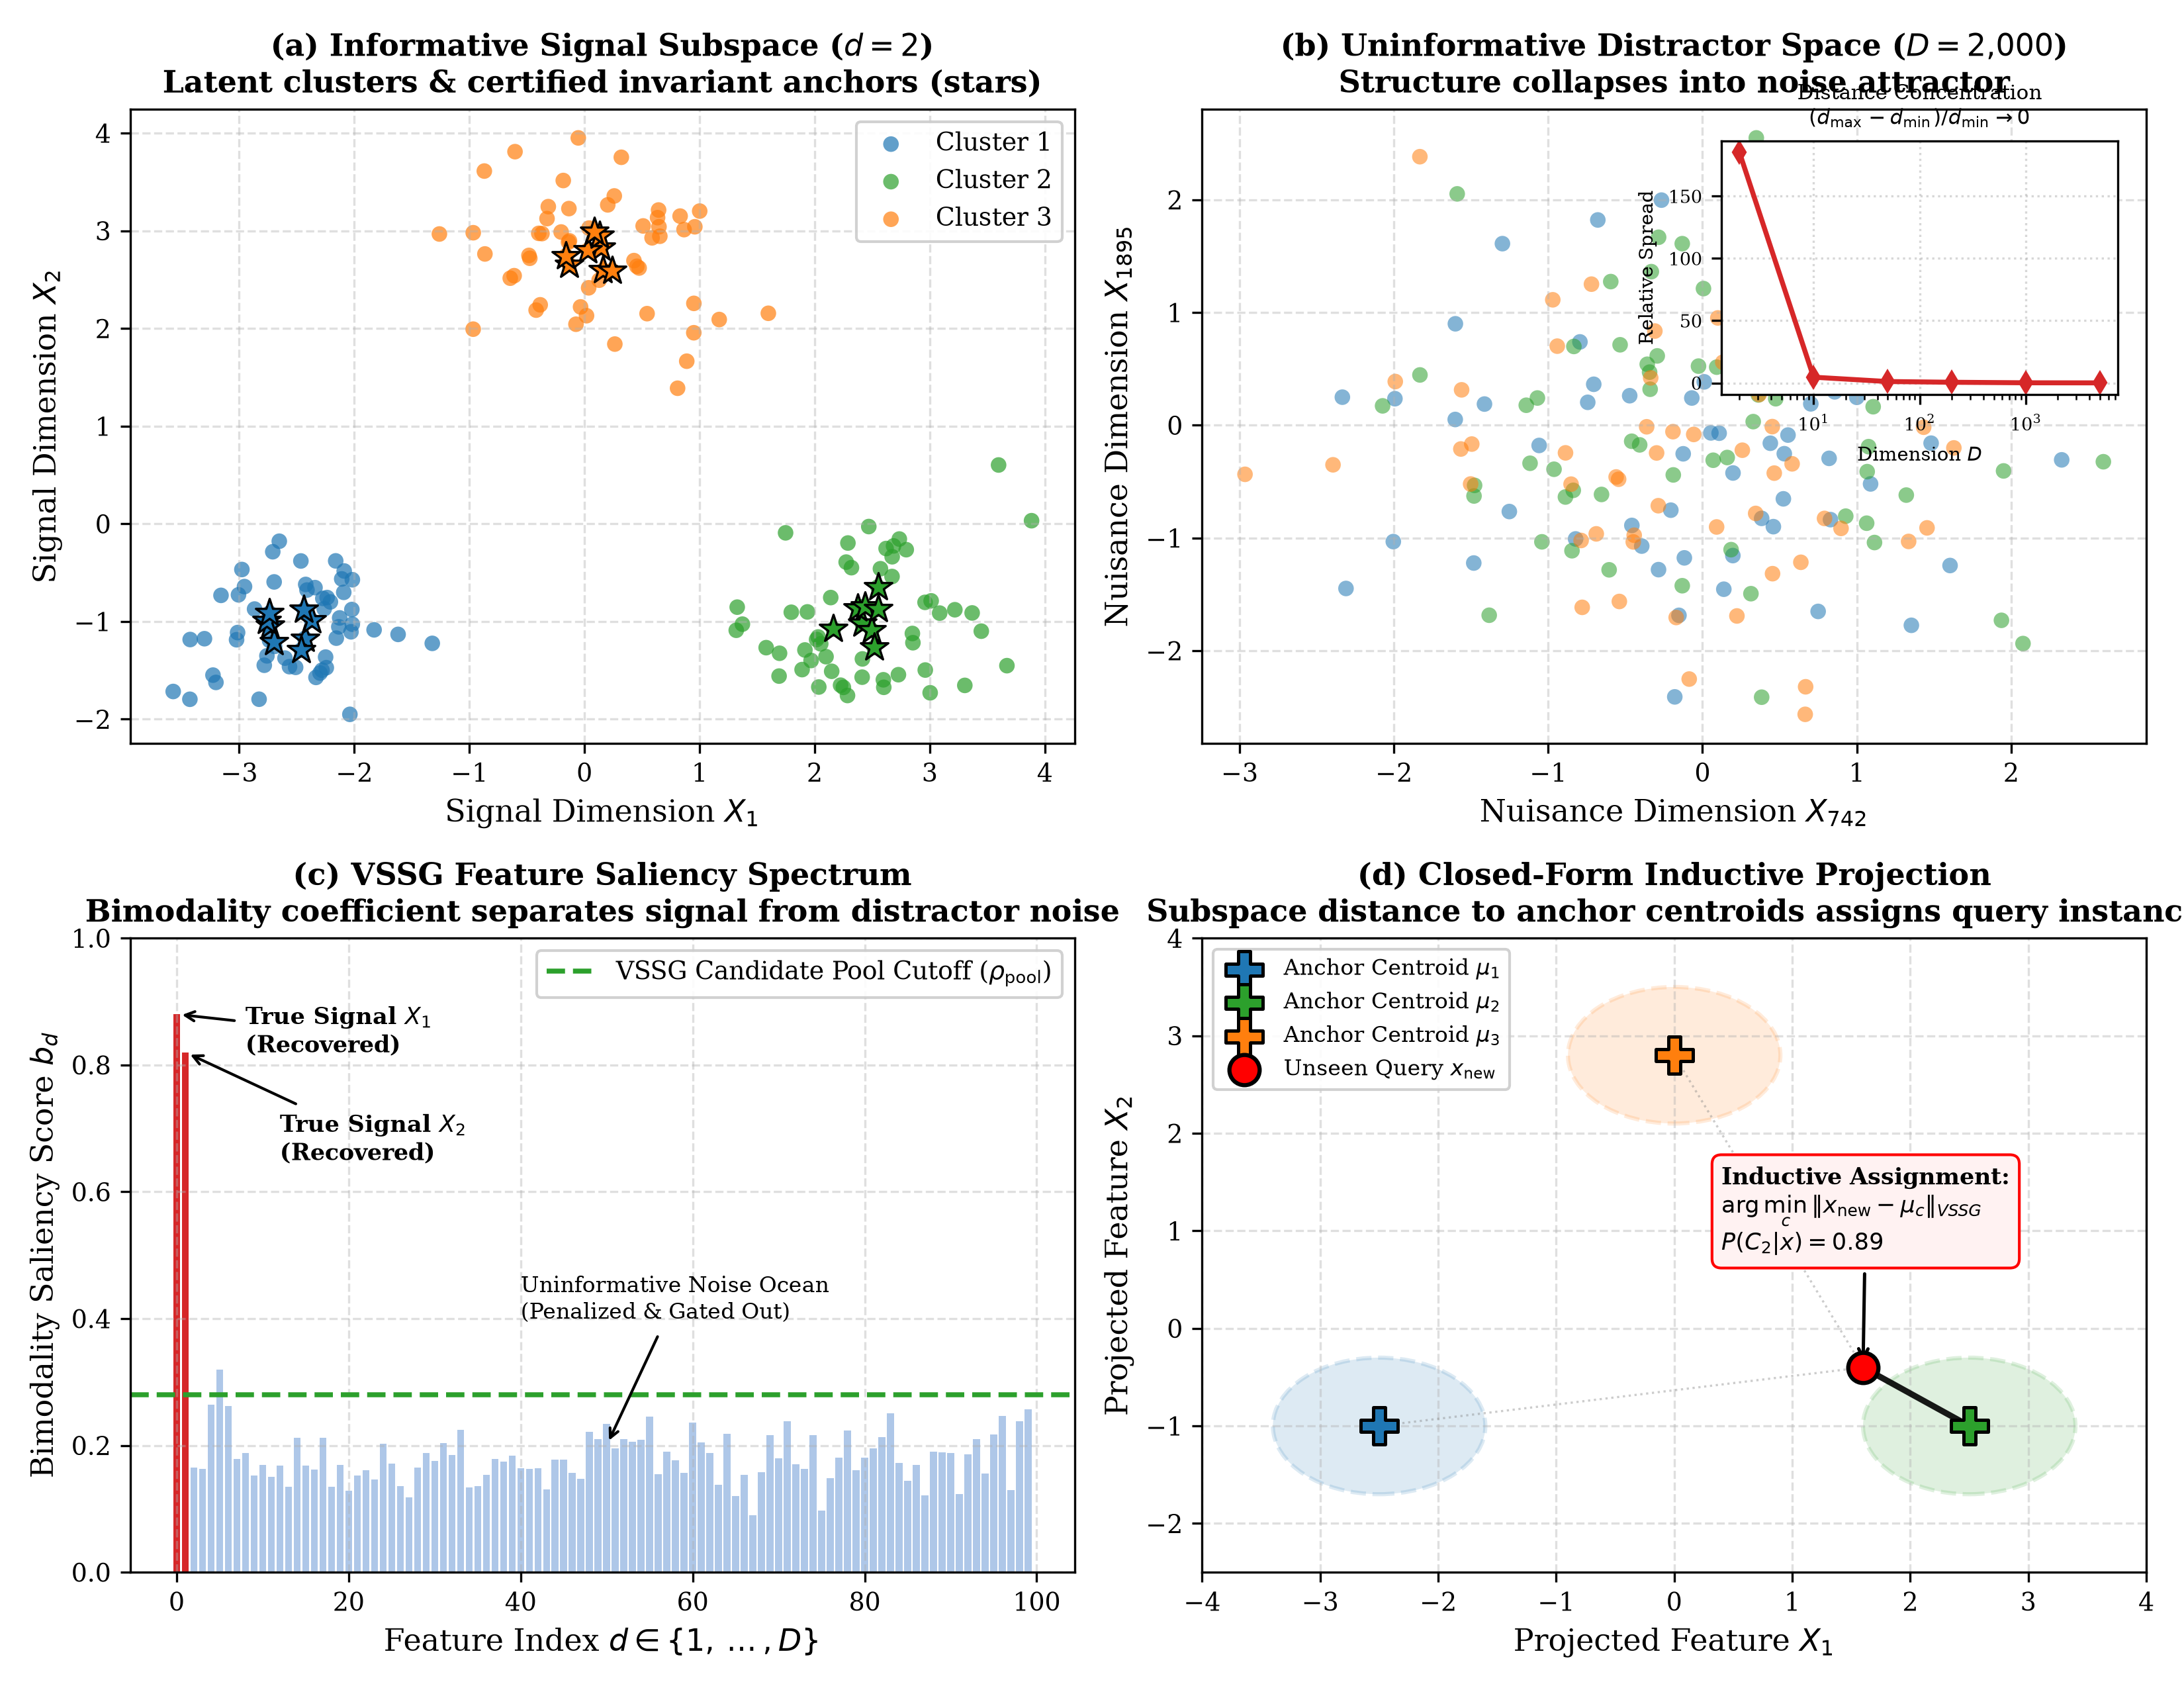
\includegraphics[width=0.96\textwidth]{figures/fig0_conceptual_framework.png}
\caption{Conceptual overview of the high-dimensional noise dilemma and the proposed Inductive Consensus Clustering (ICC-v2) framework. (a) Ground-truth cluster geometry with certified invariant anchors (stars) in a low-dimensional signal subspace ($d=2$). (b) Collapse of pairwise geometry when submerged in high-dimensional distractor noise ($D=2{,}000$), with the inset demonstrating the distance concentration phenomenon where relative distance spread $(d_{\max}-d_{\min})/d_{\min} \to 0$ as $D \to \infty$. (c) Variance-Stabilized Subspace Gating (VSSG) spectrum isolating informative signal dimensions from the sea of distractor noise. (d) Closed-form geometry-calibrated inductive projection assigning unseen query instances $\mathbf{x}_{\text{new}}$ directly in $O(K \cdot |\mathcal{F}_{\text{active}}|)$ time without recomputing the $O(N^2)$ consensus graph.}
\label{fig:conceptual_overview}
\end{figure*}

To overcome these foundational limitations, this paper develops the \textbf{Inductive Consensus Clustering (ICC)} framework (Fig.~\ref{fig:conceptual_overview}). We first examine the finite-sample empirical breakdown of consensus stability under isotropic distractor noise (Exp~0), illustrating how distance concentration generates deceptive consensus stability on arbitrary noise boundaries. Motivated by these empirical findings, we architect \textbf{ICC-v2}, a unified four-stage framework:
\begin{itemize}
    \item \textbf{Variance-Stabilized Subspace Gating (VSSG):} An $O(N \cdot D)$ linear feature screening mechanism utilizing Sarle's Bimodality Coefficient with finite-sample null correction ($\hat{b}_d = \frac{\hat{\gamma}_d^2 + 1}{\hat{\kappa}_d + 3 \frac{(N-1)^2}{(N-2)(N-3)} + \epsilon}$) to purge unimodal distractor noise prior to base ensemble fitting.
    \item \textbf{Determinacy-Based Bipartite Anchor Consensus:} Constructs a rectangular bipartite co-association graph $B \in [0, 1]^{N \times L}$ over $L$ core anchors selected via quadratic consensus determinacy ($\sigma_i = \frac{1}{N-1}\sum_{j \neq i} S_{ij}^2$), reducing auxiliary memory from $O(N^2)$ to $O(N \cdot L)$ and accelerating spectral decomposition onto an $L \times L$ core affinity space.
    \item \textbf{Stability-Weighted Subspace Centroid Assignment:} Provides closed-form inductive out-of-sample mapping that assigns unseen query instances in $O(K \cdot |\mathcal{F}_{\text{active}}|)$ time without recomputing the consensus graph.
    \item \textbf{Anchor-Space Perturbation Profiling (ASPP):} Probes cluster structural resilience across five physical perturbation families directly over certified anchor coordinates, delivering interpretable perturbation sensitivity indices ($PSI_k$) and calibrated out-of-sample query confidence without quadratic overhead.
\end{itemize}

Following this introduction (Section~\ref{sec:intro}), the remainder of this manuscript is structured as follows: Section~\ref{sec:related} reviews related work. Section~\ref{sec:falsification} presents our empirical analysis of distance concentration and consensus failure. Section~\ref{sec:framework} details the mathematical architecture and complexity analysis of ICC-v2, including Anchor-Space Perturbation Profiling (Section~\ref{sec:aspp}). Section~\ref{sec:experiments} provides comprehensive empirical evaluations across generalization, ablation, real-world benchmarks, and scalability. Section~\ref{sec:conclusion} concludes the paper.


\section{Related Work}\label{sec:related}

\subsection{Cluster Ensembles and Consensus Graphs}
The core consensus clustering paradigm constructs a co-association matrix $S$ where $S_{ij} = \frac{1}{M}\sum_{m=1}^M \mathbf{1}\{\pi_m(\mathbf{x}_i) = \pi_m(\mathbf{x}_j)\}$ represents the empirical probability that objects $\mathbf{x}_i$ and $\mathbf{x}_j$ are co-clustered across $M$ base partitions~\cite{fred2005combining}. Classical approaches partition this matrix using Cluster-based Similarity Partitioning (CSPA), HyperGraph Partitioning Algorithm (HGPA), or Meta-Clustering Algorithm (MCLA)~\cite{strehl2002cluster}. More recent works explore dense subgraph discovery~\cite{liu2017spectral}, random walk probability trajectories~\cite{huang2015robust}, and bipartite graph modeling~\cite{fern2004solving}. However, all these classical frameworks remain fundamentally transductive, requiring quadratic $O(N^2)$ co-association storage.

\subsection{Robust, Core-Based, and Anchor Clustering}
To withstand noise and outliers, Li et al.~\cite{li2019determinacy} proposed determinacy core spectral ensemble clustering, which partitions samples into deterministic core points and boundary points based on co-association variance. While effective in low-dimensional spaces, determinacy metrics degrade rapidly when high-dimensional noise corrupts the ensemble partitions. In scalable single-model clustering, anchor graph methods (e.g., Nie et al.~\cite{nie2024fast}, Huang et al.~\cite{huang2023fast}) utilize bipartite graphs to reduce spectral decomposition complexity. However, existing anchor methods operate on raw ambient feature spaces, leaving them vulnerable to high-dimensional noise. As summarized in Table~\ref{tab:taxonomy_comparison}, ICC-v2 is the first framework to integrate non-parametric multimodality subspace gating, determinacy-based bipartite anchor consensus, and inductive centroid projection into a unified linear-time pipeline.

\begin{table}[!t]
\caption{Methodological Taxonomy and Comparison Across Consensus Paradigms}
\label{tab:taxonomy_comparison}
\centering
\begin{tabular}{lccccc}
\toprule
\textbf{Method} & \textbf{Feature Gating} & \textbf{Core Filtering} & \textbf{Inductive Ext.} & \textbf{Memory} & \textbf{Robust ($D \gg N$)} \\
\midrule
Std Cons.~\cite{fred2005combining}   & None        & None         & No  & $O(N^2)$ & No  \\
Li et al.~\cite{li2019determinacy}   & None        & Determinacy  & No  & $O(N^2)$ & No  \\
FCAG~\cite{nie2024fast}              & None        & Anchors      & No  & $O(NL)$  & No  \\
FastMVC~\cite{huang2023fast}         & None        & Anchors      & No  & $O(NL)$  & No  \\
\textbf{ICC-v2 (Ours)}               & \textbf{VSSG (Linear)} & \textbf{Anchors} & \textbf{Yes (Centroid)} & $\mathbf{O(NL)}$ & \textbf{Yes} \\
\bottomrule
\end{tabular}
\end{table}


\section{Theoretical Motivation \& Empirical Falsification}\label{sec:falsification}

\begin{figure*}[!t]
\centering
\subfloat[Clustering Accuracy (ARI vs. Ground Truth) and Ensemble Stability Across $D_{\text{noise}}$\label{fig:ari_stability}]{%
    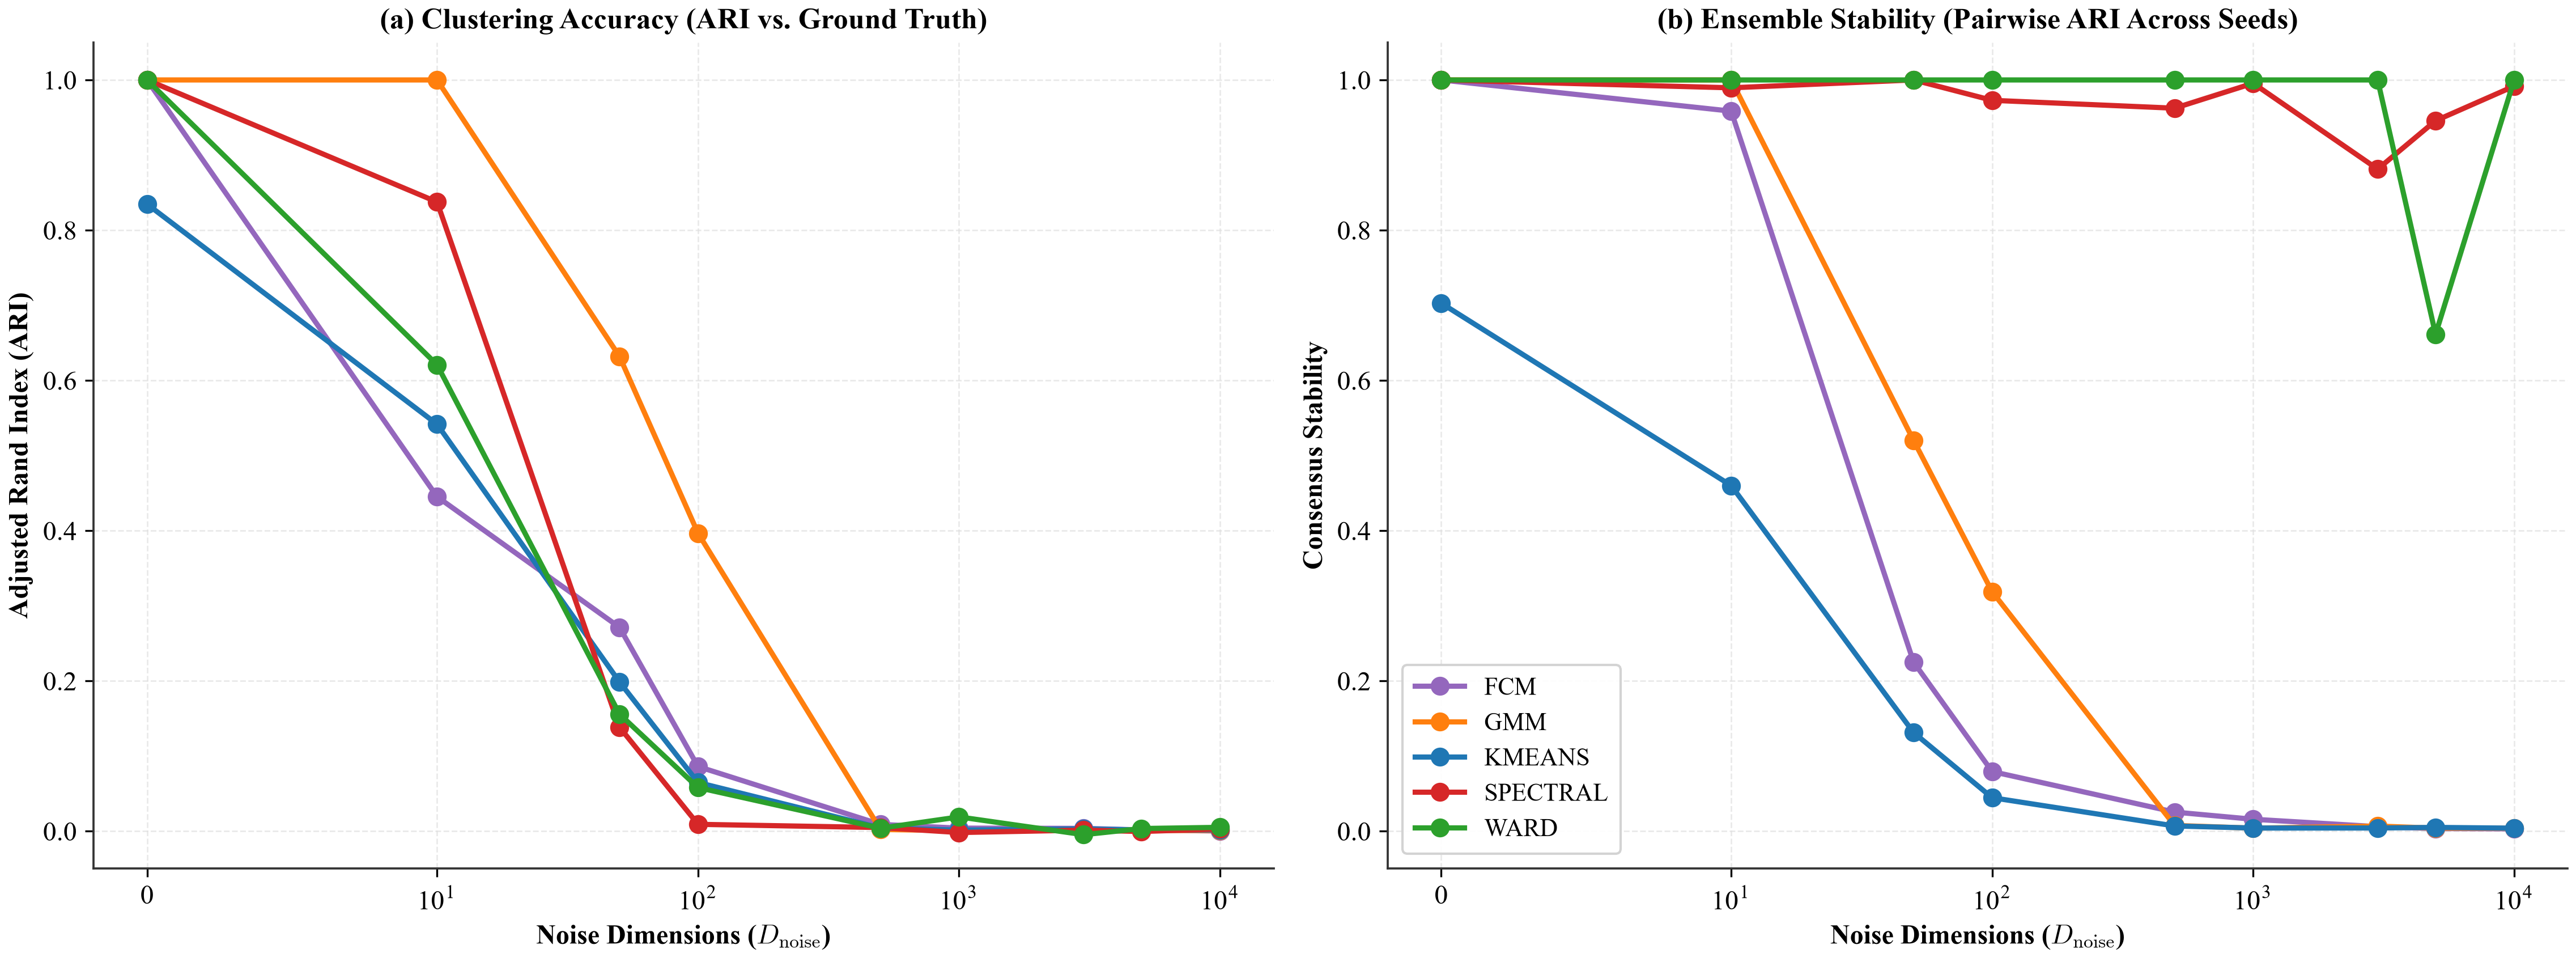
\includegraphics[width=0.96\textwidth]{figures/fig1_ari_stability.png}%
}
\\[1.5ex]
\subfloat[Stability$-$Accuracy Gap ($\Delta = \text{Stability} - \text{ARI}$)\label{fig:dist_gap}]{%
    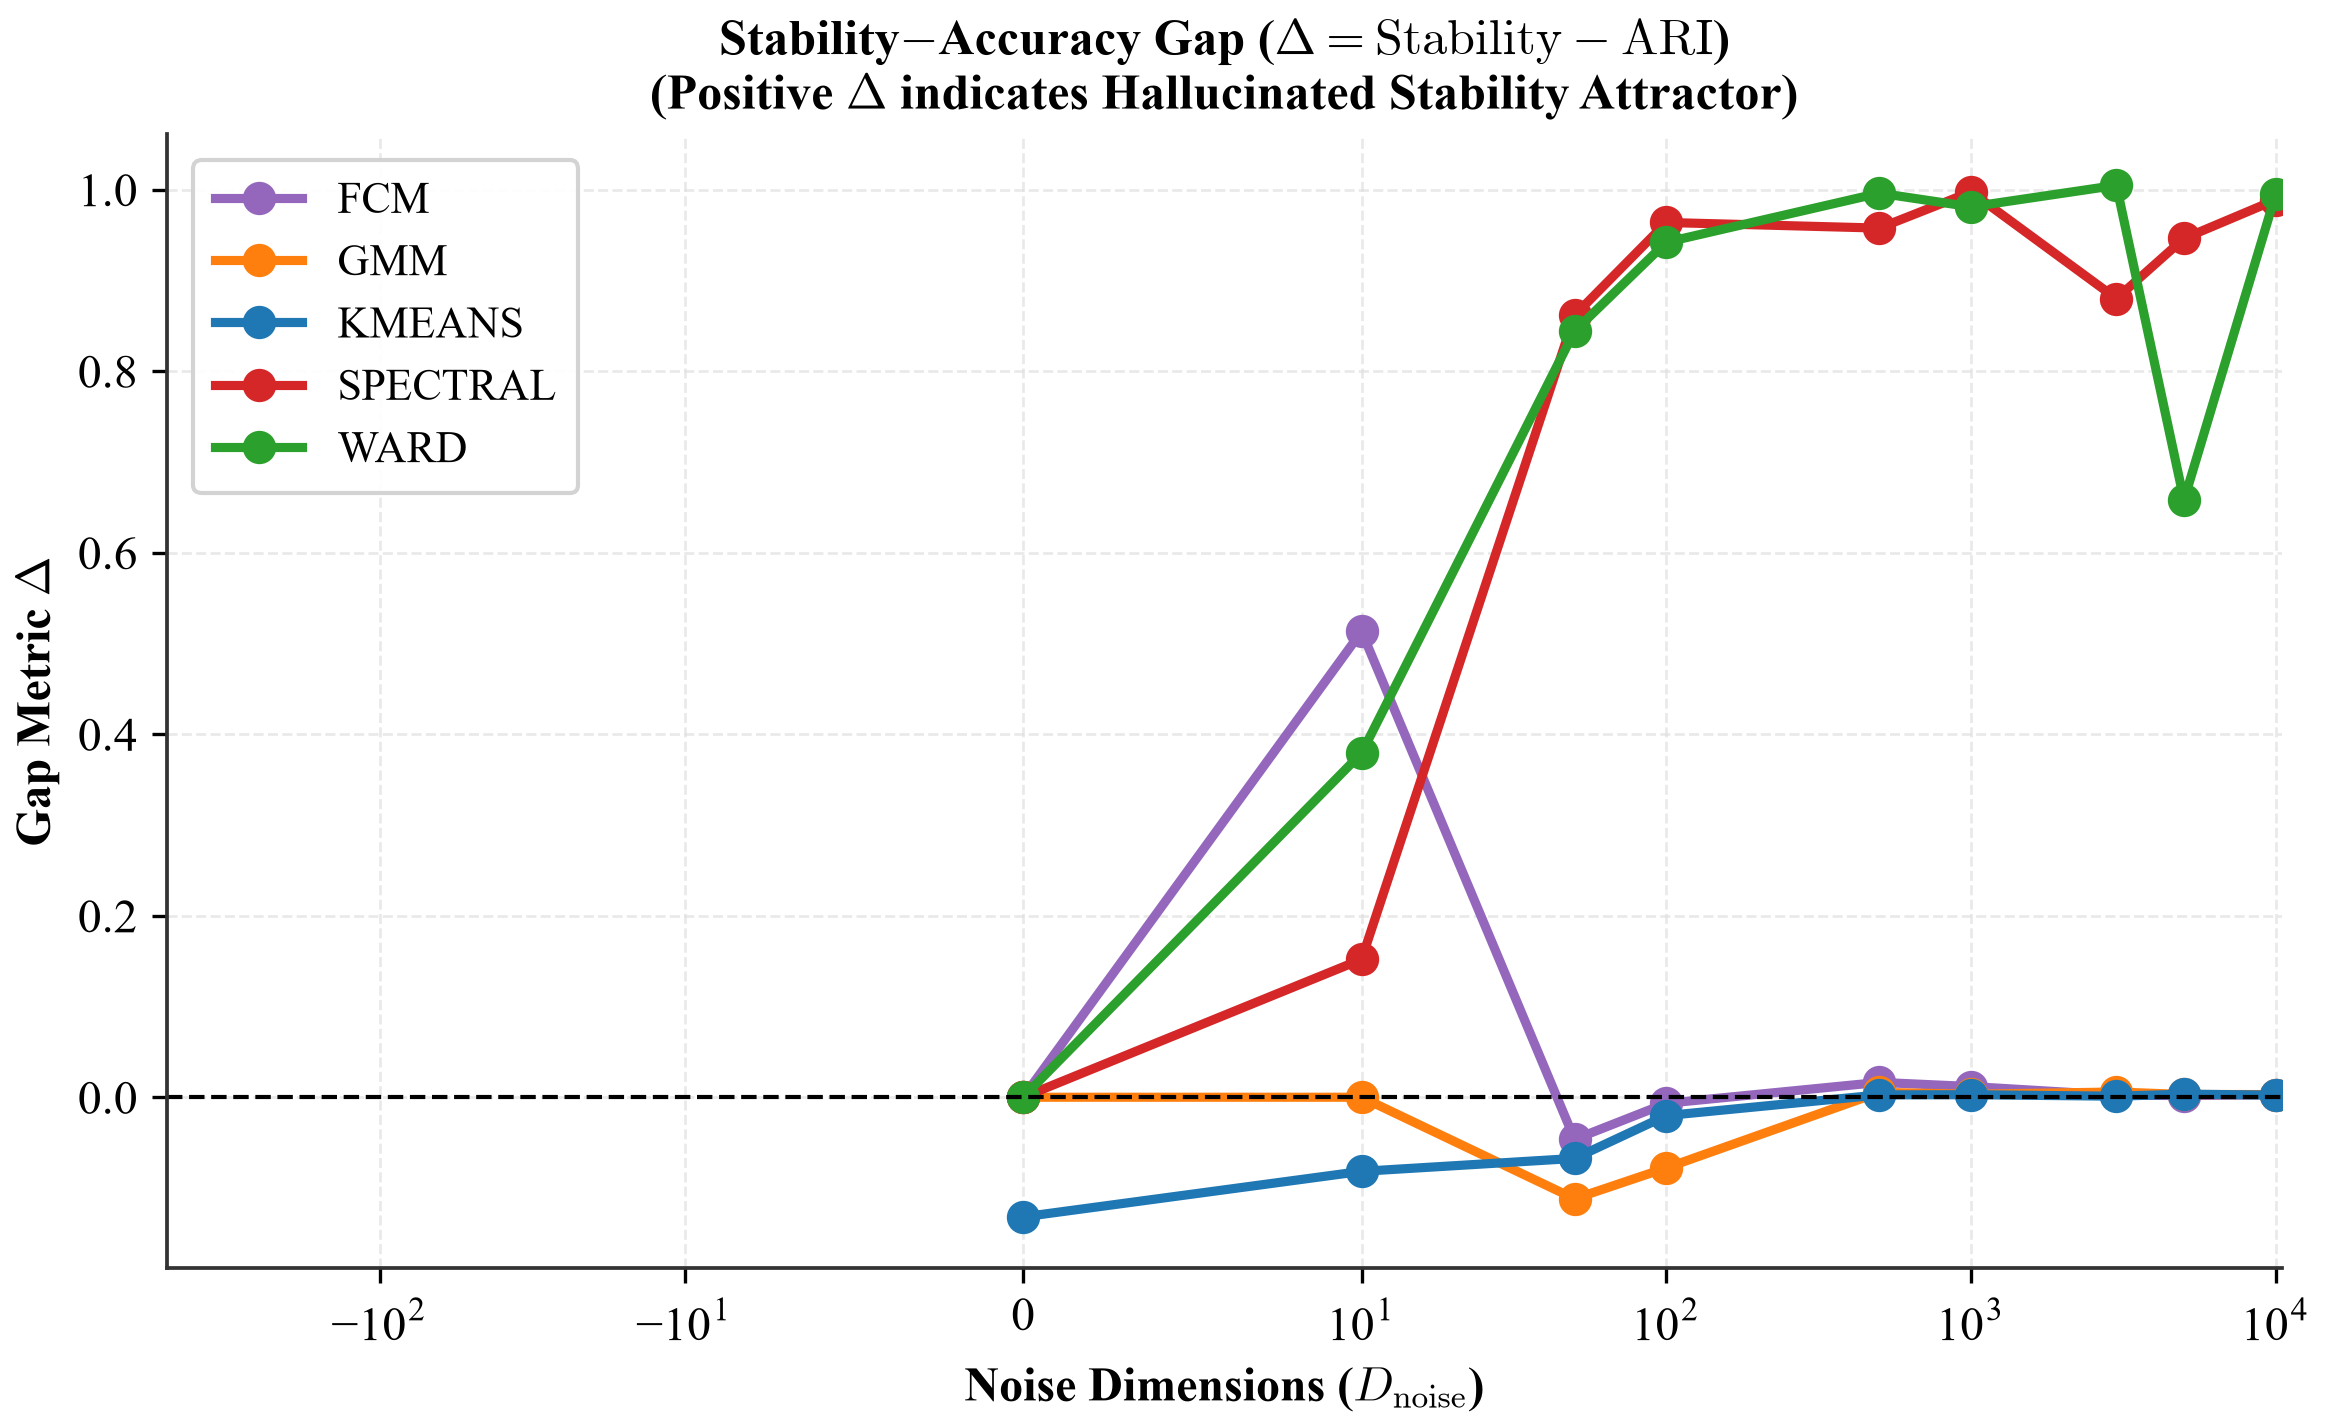
\includegraphics[width=0.48\textwidth]{figures/fig2_gap.png}%
}
\hfill
\subfloat[Noise Distribution Sensitivity Matrix ($D_{\text{noise}}=1{,}000$)\label{fig:noise_heatmap}]{%
    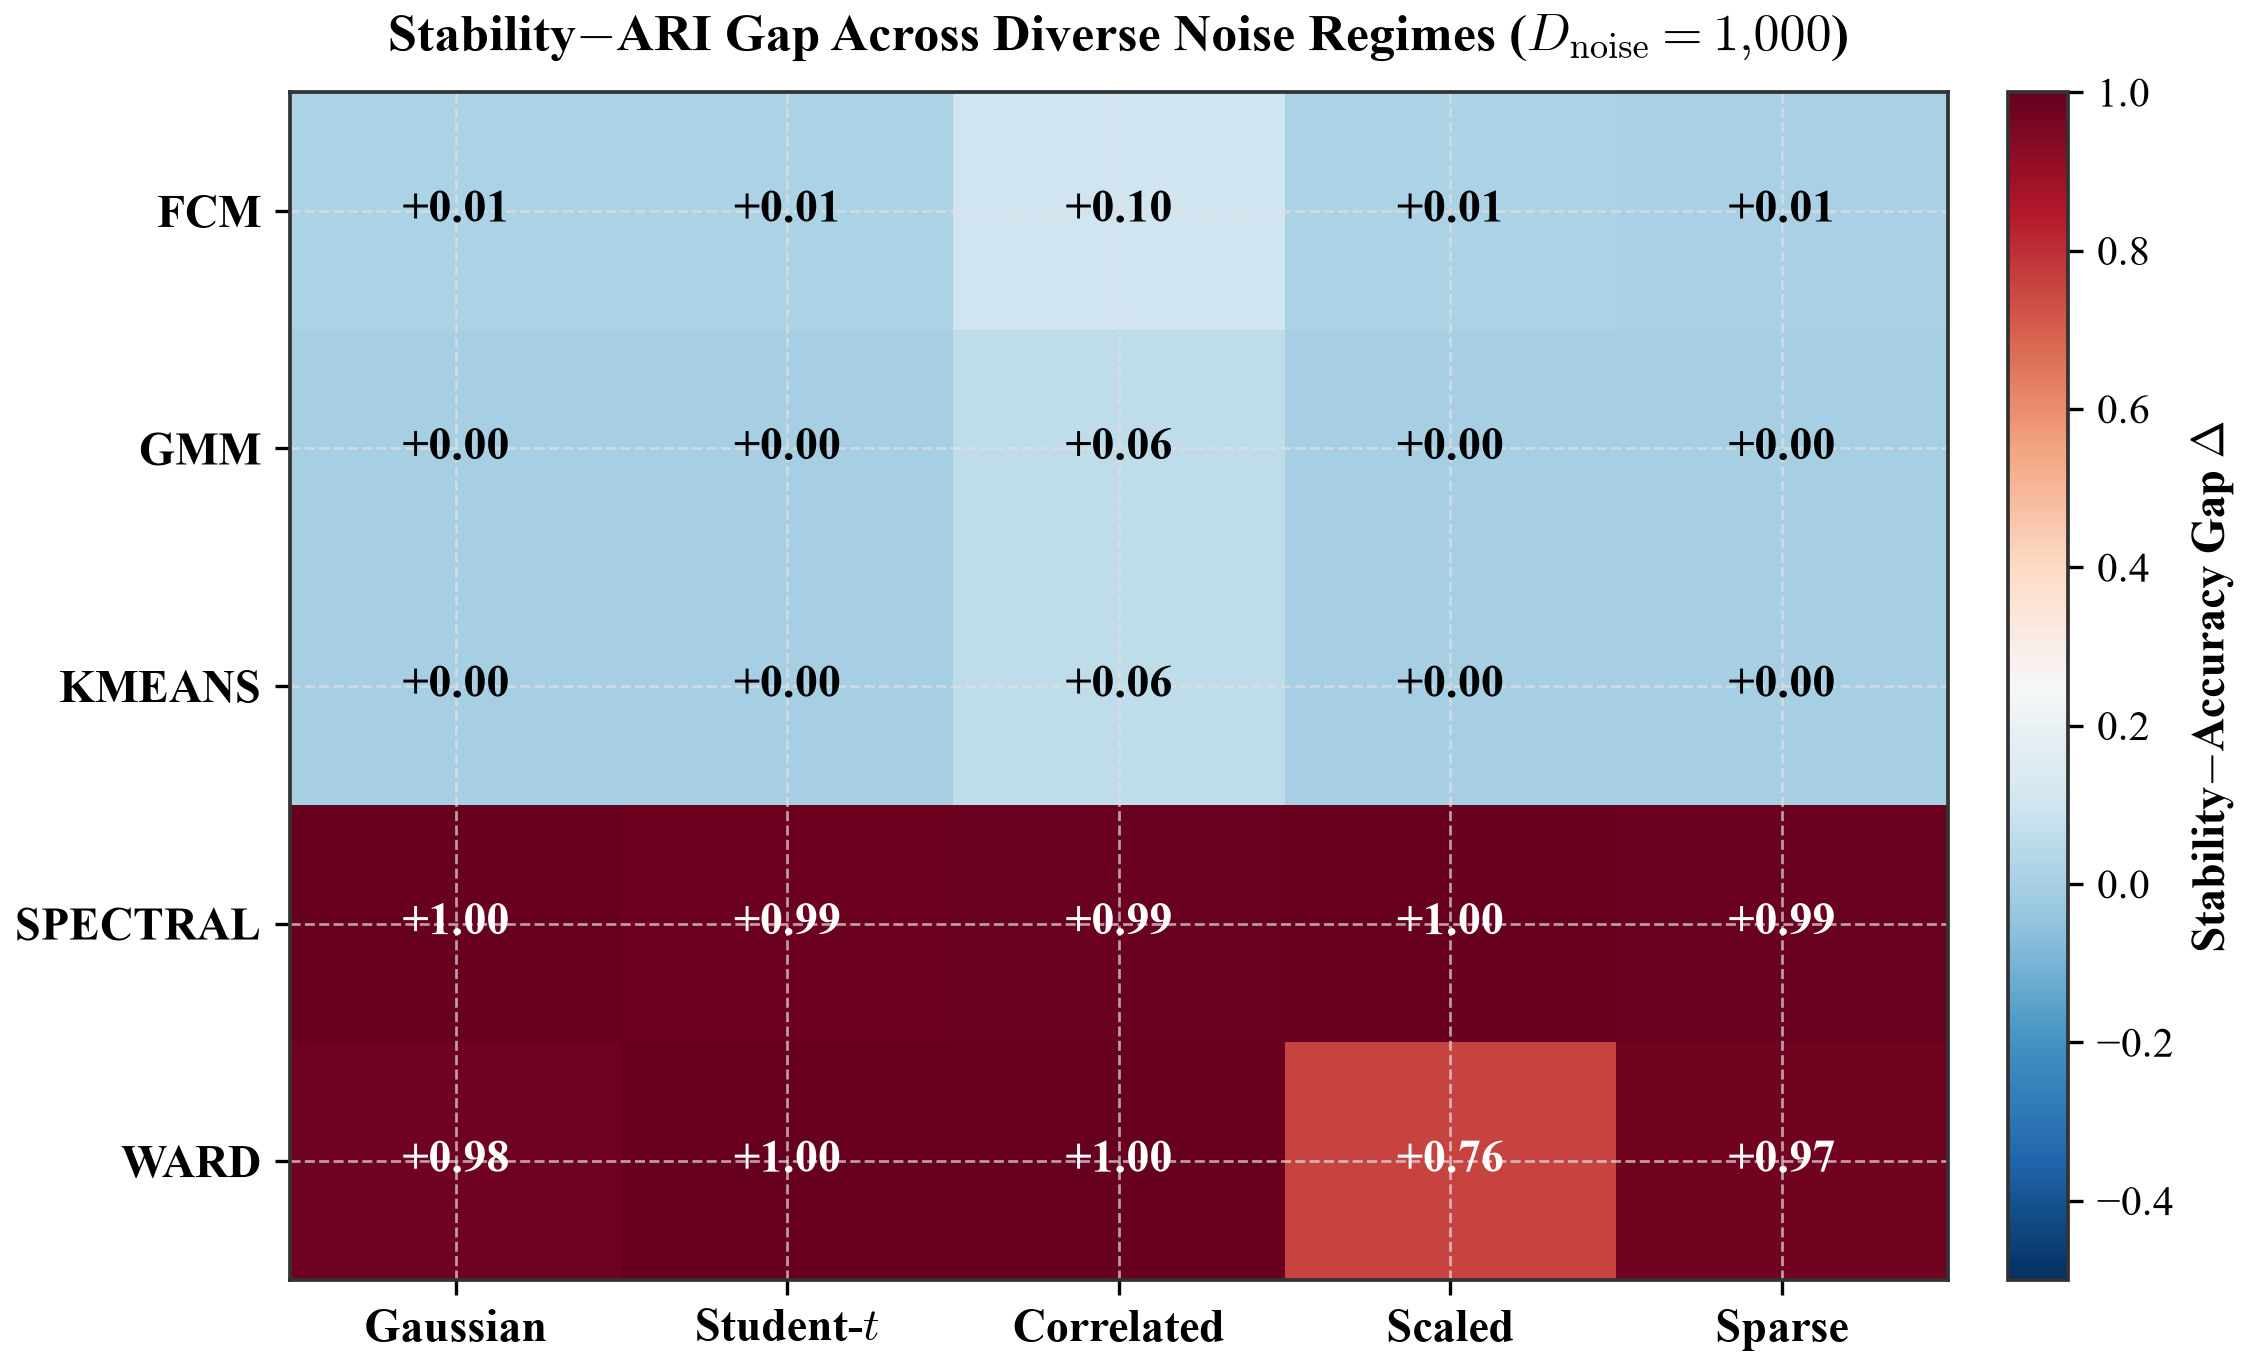
\includegraphics[width=0.48\textwidth]{figures/fig4_noisetype_heatmap.png}%
}
\caption{Empirical falsification of asymptotic consensus stability under finite-sample isotropic noise. (a) Rapid collapse of ARI stability as distractor dimensions grow, demonstrating that multi-clusterer averaging alone cannot prevent failure. (b) Gap metric confirming positive stability attractors ($\Delta > 0$). (c) Stability$-$ARI gap evaluated across diverse noise distributions.}
\label{fig:falsification_suite}
\end{figure*}

Theoretical literature on random projection clustering often asserts asymptotic recovery guarantees under the assumption of infinite samples ($N \to \infty$) or perfectly orthogonal noise. We conducted rigorous falsification experiments (Exp~0) on finite-sample datasets to systematically test whether consensus averaging alone protects against high-dimensional distractor noise.

\begin{definition}[Within/Between Distance Ratio]
Let $\mathcal{C}_k$ denote cluster $k$ with centroid $\boldsymbol{\mu}_k$. For an empirical sample $X \subset \mathbb{R}^D$, the separation ratio is defined as:
\begin{equation}
    \rho_{\text{sep}}(X) = \frac{\frac{1}{K}\sum_{k=1}^K \frac{1}{|\mathcal{C}_k|}\sum_{\mathbf{x}_i \in \mathcal{C}_k} \|\mathbf{x}_i - \boldsymbol{\mu}_k\|_2}{\frac{2}{K(K-1)}\sum_{k < l} \|\boldsymbol{\mu}_k - \boldsymbol{\mu}_l\|_2}.
\end{equation}
\end{definition}

As ambient distractor dimensions $D_{\text{noise}}$ expand ($D \gg N$), pairwise Euclidean distances suffer from distance concentration~\cite{beyer1999nearest}, where the relative contrast (coefficient of variation) of distances vanishes: $\lim_{D \to \infty} \frac{\mathrm{Var}(\|\mathbf{x}_i - \mathbf{x}_j\|_2)}{\mathbb{E}[\|\mathbf{x}_i - \mathbf{x}_j\|_2]^2} = 0$. Under pure isotropic noise, both within-cluster and between-cluster Euclidean distances converge to the common expectation $\sqrt{2 D \sigma^2}$, driving the separation ratio $\rho_{\text{sep}}(X)$ toward $1.0$ (Fig.~\ref{fig:dist_gap}) and rendering raw Euclidean distances indistinguishable. Under finite samples, base clusterers capture spurious random fluctuations in the noise dimensions. This induces a \textbf{hallucinated stability trap}: base partitions repeatedly converge on arbitrary noise boundaries with deceptive consensus agreement ($\text{Stability} > 0.8$), while true cluster recovery collapses ($\text{ARI} \to 0$, Fig.~\ref{fig:ari_stability}). As evaluated across diverse distractor distributions (Fig.~\ref{fig:noise_heatmap}), a positive stability$-$accuracy discrepancy ($\Delta = \text{Stability} - \text{ARI} > 0$, Fig.~\ref{fig:dist_gap}) emerges prominently for graph-based and hierarchical base clusterers (Spectral and Ward), while centroid-based partitions collapse simultaneously in both metrics. This confirms the hallucinated stability trap under Gaussian, Student-$t$, and correlated noise regimes (Fig.~\ref{fig:falsification_suite}). Thus, ensemble averaging alone is shown to be insufficient under finite samples to eliminate uninformative subspace noise without explicit feature gating.


\section{The Inductive Consensus Clustering Framework}\label{sec:framework}

\begin{algorithm}[!t]
\caption{Inductive Consensus Clustering (ICC-v2)}
\label{alg:iccv2}
\begin{algorithmic}[1]
\Require Data matrix $X \in \mathbb{R}^{N \times D}$, ensemble size $M$, target clusters $K$, anchor budget $L \ll N$ (default 40, adaptive $\max(40, 10K)$), core quantile $\tau_{\text{core}}$, candidate pool fraction $\alpha$.
\Ensure Consensus labels $\mathbf{y} \in \{1,\dots,K\}^N$, Anchors $\mathcal{A}_{\text{core}}$, Active Subspace $\mathcal{F}_{\text{active}}$, Centroids $\{\boldsymbol{\mu}_k\}_{k=1}^K$.
\Statex \textbf{// Stage 1: Multimodality Subspace Gating (VSSG)}
\For{each feature column $d \in \{1,\dots,D\}$}
    \State Compute Sarle's Bimodality Coefficient:
    \State $\hat{b}_d \leftarrow \frac{\hat{\gamma}_d^2 + 1}{\hat{\kappa}_d + 3 \frac{(N-1)^2}{(N-2)(N-3)} + \epsilon}$.
\EndFor
\State Extract candidate pool $\mathcal{F}_{\text{active}} \leftarrow \{d \mid \hat{b}_d \ge 5/9\}$ (capped at top $\min(D, \max(100, \lfloor 0.15 D \rfloor))$).
\Statex \textbf{// Stage 2: Guided Subspace Ensemble Generation}
\For{$m = 1$ to $M$}
    \State Draw random subspace $\mathcal{F}_m \subset \mathcal{F}_{\text{active}}$.
    \State Fit base partition $\pi_m \leftarrow \text{Clusterer}(X_{[:, \mathcal{F}_m]}, K)$.
\EndFor
\Statex \textbf{// Stage 3: Determinacy-Based Bipartite Anchor Consensus}
\State Evaluate exact determinacy $\sigma_i \leftarrow \frac{1}{N-1}\sum_{j \neq i} S_{ij}^2$ via Prop.~2 contingency identity in $O(M^2 N + M^2 K^2)$.
\State Select $L = \min(L_{\text{budget}}, |\mathcal{A}_{\text{core}}|)$ core anchors (default $L=40$, adaptive $L=\max(40, 10K)$) from certified core $\{i \mid \sigma_i \ge \text{Quantile}(\boldsymbol{\sigma}, \tau_{\text{core}})\}$.
\State Construct bipartite co-association matrix $B \in [0, 1]^{N \times L}$:
\State $B_{ia} \leftarrow \frac{1}{M}\sum_{m=1}^M \mathbf{1}\{\pi_m(\mathbf{x}_i) = \pi_m(\mathbf{x}_a)\}$.
\State Row-normalize $B_{\text{norm}} \leftarrow \Delta_R^{-1} B$, and compute $W_{\text{anchor}} \leftarrow B_{\text{norm}}^T B_{\text{norm}} \in \mathbb{R}^{L \times L}$.
\State Solve normalized Laplacian $L_{\text{anchor}} \leftarrow I_L - \Delta_A^{-1/2} W_{\text{anchor}} \Delta_A^{-1/2}$ for eigenvectors $V \in \mathbb{R}^{L \times K}$ of the $K$ smallest eigenvalues.
\State Compute instance embedding $U \leftarrow B_{\text{norm}} \Delta_A^{-1/2} V \Sigma^{-1/2} \in \mathbb{R}^{N \times K}$ (row-normalized).
\State Extract consensus labels $\mathbf{y} \leftarrow \text{K-Means}(U, K)$.
\Statex \textbf{// Stage 4: Stability-Weighted Centroid Induction}
\For{$k = 1$ to $K$}
    \State $\boldsymbol{\mu}_k \leftarrow \frac{\sum_{i: y_i = k} \sigma_i \cdot \mathbf{x}_{i, [\mathcal{F}_{\text{active}}]}}{\sum_{i: y_i = k} \sigma_i}$.
\EndFor
\State \Return $\mathbf{y}, \mathcal{A}_{\text{core}}, \mathcal{F}_{\text{active}}, \{\boldsymbol{\mu}_k\}_{k=1}^K$.
\Statex \textbf{// Out-of-Sample Inference for Query $\mathbf{x}^* \in \mathbb{R}^D$:}
\State \textbf{predict}($\mathbf{x}^*$): \Return $\arg\min_k \|\mathbf{x}^*_{[\mathcal{F}_{\text{active}}]} - \boldsymbol{\mu}_k\|_2$.
\end{algorithmic}
\end{algorithm}

The ICC-v2 framework (Algorithm~\ref{alg:iccv2}) operates in four distinct stages:

\subsection{Variance-Stabilized Subspace Gating (VSSG)}
Under isotropic noise in $D \gg N$ regimes, classical variance thresholding fails because distractor noise features often match or exceed signal feature variances. To detect latent cluster structures without labels, VSSG evaluates marginal multimodality using \textbf{Sarle's Bimodality Coefficient} ($BC$)~\cite{sarle1983sas} with finite-sample null correction:
\begin{equation}
    \hat{b}_d = \frac{\hat{\gamma}_d^2 + 1}{\hat{\kappa}_d + 3 \cdot \frac{(N-1)^2}{(N-2)(N-3)} + \epsilon},
\end{equation}
where $\hat{\gamma}_d$ is empirical sample skewness, $\hat{\kappa}_d$ is Fisher's excess kurtosis, and the denominator represents Pearson kurtosis $\hat{\beta}_{2, d}$ adjusted for finite-sample normal null expectations. Features with zero variance ($\mathrm{Var}(\mathbf{f}_d) < 10^{-12}$) are assigned $\hat{b}_d = 0$.

\begin{proposition}[Conditional Multimodality Separation Bound]\label{prop:multimodality_bound}
For a standard unimodal Gaussian distractor distribution, $\gamma = 0$ and $\kappa = 0$, yielding $\mathbb{E}[\hat{b}_d] \approx 1/3 \approx 0.333$. For a continuous uniform distribution, $b_d = 5/9 \approx 0.555$. For an equal-weight two-component Gaussian mixture $0.5\mathcal{N}(-\Delta, \sigma^2) + 0.5\mathcal{N}(\Delta, \sigma^2)$, exact moment derivation reveals that the bimodality coefficient satisfies $b_d > 5/9$ if and only if normalized component separation satisfies $r = \Delta^2 / \sigma^2 > (3 + \sqrt{15})/2 \approx 3.436$, corresponding to separation ratio $\Delta / \sigma > \sqrt{(3+\sqrt{15})/2} \approx 1.854$. For asymmetric two-component mixtures with weights $w \in (0, 1)$ and $1-w$, skewness is non-zero ($\gamma \neq 0$), shifting the critical threshold upward as imbalance increases; as $w(1-w) \to 0$, extreme component separation is required to cross $5/9$. For general multi-component mixtures ($K > 2$), marginal multimodality emerges when adjacent centroid gaps exceed $|\mu_k - \mu_{k-1}| > 1.854 \sigma$.
\end{proposition}

Computing $\hat{b}_d$ requires only empirical second, third, and fourth moments across instances, executing in strictly \textbf{$O(N \cdot D)$ time} with zero quadratic distance computations. We formalize the foundational inductive bias and boundary conditions of VSSG:
\begin{assumption}[Marginal Multimodality Prior]\label{assump:multimodal}
Informative subspace dimensions separating ground-truth clusters exhibit marginal multimodality ($\hat{b}_d \ge 5/9$), whereas uninformative nuisance distractor dimensions are continuous and unimodal ($\hat{b}_d \le 5/9$).
\end{assumption}

\begin{remark}[Theoretical Failure Modes of Marginal Bimodality Gating]\label{rem:vssg_failures}
Assumption~\ref{assump:multimodal} imposes an inductive filter that exhibits three specific failure boundaries:
\begin{enumerate}
    \item \textbf{Skewed Unimodal Distributions:} High marginal skewness $\hat{\gamma}_d$ (e.g., in lognormal distributions, Pareto tails, or zero-inflated expression counts) mathematically inflates $\hat{b}_d \ge 5/9$ because Sarle's index scales with $(\gamma^2+1)/\beta_2$, falsely tagging skewed unimodal noise as multimodal.
    \item \textbf{Non-Linear Parity / XOR Manifolds:} In multivariate parity problems (such as the Madelon benchmark comprising 5 informative hypercube vertices, 15 redundant linear combinations, and 480 distractor noise features), cluster identity depends on joint feature configurations whose 1D marginals are strictly unimodal. Consequently, 1D screening cannot detect pure XOR parity coordinates, bounding marginal discovery ($\text{Recall}@K$ peaks at $\sim 0.45$).
    \item \textbf{Finite-Sample Estimator Variance ($N \le 100$):} In small sample sizes, sample skewness and kurtosis estimators exhibit high sampling variance, causing occasional false-positive threshold crossings. This motivates the finite-sample normal null correction $3\frac{(N-1)^2}{(N-2)(N-3)}$ and strict pool size capping.
\end{enumerate}
\end{remark}

\begin{remark}[Sparsity and Zero-Inflation Boundary]
Under highly sparse or zero-inflated representations (e.g., raw TF-IDF document vectors or single-cell counts with $\ge 90\%$ zeros), the discrete point mass at zero inflates skewness and kurtosis, causing marginal $\hat{b}_d$ scores to degrade. In such regimes, dense continuous representation learning or latent semantic indexing should precede subspace gating.
\end{remark}

Under Assumption~\ref{assump:multimodal}, VSSG selects candidate dimensions via null-calibrated thresholding $\hat{b}_d \ge 5/9$ (capped at an active pool size of at most $\min(D, \max(100, \lfloor 0.15 D \rfloor))$), or via top-fraction ranking $\text{TopRank}(\hat{b}, \max(K, \lfloor \alpha D \rfloor))$, ensuring base clusterers operate on signal-rich subspaces.

\subsection{Determinacy-Based Bipartite Anchor Consensus}
Classical consensus methods construct a dense $N \times N$ co-association matrix $S$ and perform graph partitioning in $O(N^2)$ to $O(N^3)$ time and $O(N^2)$ auxiliary memory. Rather than materializing all-pairs co-association, ICC-v2 evaluates exact sample determinacy $\sigma_i = \frac{1}{N - 1} \sum_{j \neq i} S_{ij}^2$ in linear memory.

\begin{proposition}[Exact Linear-Memory Determinacy Identity]\label{prop:linear_determinacy}
Let $P \in \{0, \dots, K-1\}^{M \times N}$ denote the ensemble partition matrix. Let $C_{m_1, m_2} \in \mathbb{N}^{K \times K}$ denote the contingency matrix between base partitions $m_1$ and $m_2$, where $C_{m_1, m_2}(c_1, c_2) = \sum_{j=1}^N \mathbf{1}\{\pi_{m_1}(j)=c_1 \wedge \pi_{m_2}(j)=c_2\}$. Then for every sample $i$, the quadratic determinacy satisfies the exact identity:
\begin{equation}
    \sum_{j=1}^N S_{ij}^2 = \frac{1}{M^2} \sum_{m_1=1}^M \sum_{m_2=1}^M C_{m_1, m_2}(\pi_{m_1}(i), \pi_{m_2}(i)),
\end{equation}
which computes exact sample determinacy $\sigma_i = \frac{1}{N-1}\left(\sum_{j=1}^N S_{ij}^2 - 1\right)$ in $O(M^2 N + M^2 K^2)$ time and $O(N + K^2)$ working memory, without materializing the $N \times N$ matrix $S$.
\end{proposition}

Given the exact sample stability vector $\boldsymbol{\sigma} \in [0, 1]^N$ established by Proposition~\ref{prop:linear_determinacy}, ICC-v2 extracts a core anchor set $\mathcal{A}_{\text{core}} = \{a_1, \dots, a_L\}$ of size $L \ll N$ (default benchmark configuration uses $L=40$; adaptive mode sets $L=\max(40, 10K)$) from samples exceeding stability quantile $\tau_{\text{core}}$. ICC-v2 then constructs a rectangular bipartite co-association matrix $B \in [0, 1]^{N \times L}$ where $B_{ia} = \frac{1}{M}\sum_{m=1}^M \mathbf{1}\{\pi_m(\mathbf{x}_i) = \pi_m(\mathbf{x}_a)\}$ in strictly $O(N \cdot L)$ memory.

To prevent notation clash between ambient feature dimension $D$ and graph degree matrices, let $\Delta_R = \operatorname{diag}(B \mathbf{1}_L) \in \mathbb{R}^{N \times N}$ denote the row-sum normalization matrix, yielding $B_{\text{norm}} = \Delta_R^{-1} B$. The anchor affinity matrix is $W_{\text{anchor}} = B_{\text{norm}}^T B_{\text{norm}} \in \mathbb{R}^{L \times L}$, with diagonal degree matrix $\Delta_A = \operatorname{diag}(W_{\text{anchor}} \mathbf{1}_L) \in \mathbb{R}^{L \times L}$. Following bipartite Transfer-Cut spectral theory~\cite{li2015transfer,nie2024fast}, we construct the normalized anchor Laplacian $L_{\text{anchor}} = I_L - \Delta_A^{-1/2} W_{\text{anchor}} \Delta_A^{-1/2}$ and solve for the eigenvectors $V \in \mathbb{R}^{L \times K}$ corresponding to the $K$ \textbf{smallest eigenvalues} $\lambda_1 \le \dots \le \lambda_K$ (equivalent to the largest eigenvectors of the normalized affinity operator). The dual instance embedding is given by:
\begin{equation}
    U = B_{\text{norm}} \Delta_A^{-1/2} V \Sigma^{-1/2} \in \mathbb{R}^{N \times K},
\end{equation}
where $\Sigma = \operatorname{diag}(\max(1 - \lambda_1, 10^{-4}), \dots, \max(1 - \lambda_K, 10^{-4}))$ prevents eigenvalue explosion near $\lambda_k = 1$, followed by unit row-normalization and final K-Means clustering.

\begin{remark}[Determinacy Anchor Concentration and Category Imbalance]\label{rem:anchor_bias}
Consensus determinacy $\sigma_i$ measures the consistency with which sample $i$ is co-partitioned across base clusterers. Consequently, samples situated in dense, well-separated, high-density clusters naturally achieve higher determinacy than samples residing in diffuse, overlapping, or minority clusters. Because $\mathcal{A}_{\text{core}}$ draws anchors without per-cluster stratification, anchors disproportionately concentrate in majority classes. In datasets with large category counts ($K \ge 16$, such as Isolet with $K=26$, 20 Newsgroups with $K=20$, and Indian Pines with $K=16$), a fixed budget of $L=40$ allocates fewer than two anchors per cluster on average, leading to minority subtype under-sampling and explaining why dense hierarchical clustering and deep models maintain an advantage on these multi-class benchmarks.
\end{remark}

\begin{theorem}[Computational and Memory Complexity of Bipartite ICC-v2]
Let $N$ be the sample size, $D$ ambient dimensionality, $M$ ensemble size, $L$ anchor budget ($L \ll N$), $K$ cluster count, and $I_{\text{km}}$ base K-Means iterations. Under bounded anchor budgets ($L = O(1)$), the overall time complexity of ICC-v2 is:
\begin{equation}\label{eq:complexity}
\begin{split}
    T_{\text{ICC-v2}} = O\bigl(&N D + M I_{\text{km}} N |\mathcal{F}_{\text{sub}}| K + M^2 N + M^2 K^2 \\
    &+ M N L + N L^2 + L^3 + N L K + I_{\text{km}} N K^2\bigr),
\end{split}
\end{equation}
which scales strictly linearly with sample size $O(N)$. The auxiliary working memory complexity is $O(N L + L^2)$, representing an asymptotic $O(N)$ bound that eliminates the $O(N^2)$ storage bottleneck of dense consensus.
\end{theorem}

\begin{proof}
Stage 1 (VSSG) evaluates moments in $O(N D)$. Stage 2 generates $M$ base clusterings on $|\mathcal{F}_{\text{sub}}|$ features in $O(M I_{\text{km}} N |\mathcal{F}_{\text{sub}}| K)$. Stage 3 evaluates exact sample determinacy in $O(M^2 N + M^2 K^2)$ via Proposition~\ref{prop:linear_determinacy}, constructs bipartite co-association $B$ in $O(M N L)$, computes anchor inner products $B_{\text{norm}}^T B_{\text{norm}}$ in $O(N L^2)$, eigensolves on $L \times L$ in $O(L^3)$, performs spectral projection $U = B_{\text{norm}} V$ in $O(N L K)$, and executes final K-Means in $O(I_{\text{km}} N K^2)$. Storing $B$ and $W_{\text{anchor}}$ requires only $N L + L^2$ memory words.
\end{proof}

\subsection{Stability-Weighted Active Subspace Centroid Assignment}
Unlike existing consensus frameworks that are strictly transductive, ICC-v2 extracts geometry-calibrated centroids in the active subspace weighted by point determinacy:
\begin{equation}
    \boldsymbol{\mu}_k = \frac{\sum_{i: y_i = k} \sigma_i \cdot \mathbf{x}_{i, [\mathcal{F}_{\text{active}}]}}{\sum_{i: y_i = k} \sigma_i}, \quad k \in \{1,\dots,K\}.
\end{equation}
Weighting by $\sigma_i$ pulls cluster centroids toward invariant core exemplars and attenuates boundary noise. For any new, unseen query instance $\mathbf{x}^* \in \mathbb{R}^D$, out-of-sample cluster assignment is computed in closed form in \textbf{$O(K \cdot |\mathcal{F}_{\text{active}}|)$ query time}:
\begin{equation}
    y^* = \arg\min_k \|\mathbf{x}^*_{[\mathcal{F}_{\text{active}}]} - \boldsymbol{\mu}_k\|_2,
\end{equation}
with posterior class probabilities computed via softmax temperature scaling with temperature $T > 0$ (default $T=1.0$):
\begin{equation}
    p(y^*=k \mid \mathbf{x}^*) = \frac{\exp(-\|\mathbf{x}^*_{[\mathcal{F}_{\text{active}}]} - \boldsymbol{\mu}_k\|_2 / T)}{\sum_{l=1}^K \exp(-\|\mathbf{x}^*_{[\mathcal{F}_{\text{active}}]} - \boldsymbol{\mu}_l\|_2 / T)}.
\end{equation}

\begin{remark}[Methodological Comparison with Existing Out-of-Sample Extensions]\label{rem:inductive_comparison}
Conventional graph-based clustering models utilize out-of-sample extensions such as Nystr\"om kernel interpolation~\cite{fowlkes2004spectral} or $k$-nearest-neighbor graph propagation~\cite{bengio2004out}. However, both approaches compute kernel similarities across the full ambient dimensionality $D$, rendering them vulnerable to high-dimensional distance concentration where ambient distractor noise dominates pairwise distances. Furthermore, Nystr\"om and $k$-NN extensions incur $O(N \cdot D)$ or $O(L \cdot D)$ distance operations per query instance. In contrast, while ICC-v2's nearest-centroid rule is conceptually straightforward, restricting the inductive mapping to the determinacy-weighted active subspace $\mathcal{F}_{\text{active}}$ confers two crucial advantages: (1) \textit{noise immunity}, by computing distances strictly over certified signal dimensions rather than ambient distractors, and (2) \textit{instant execution}, completing in $O(K \cdot |\mathcal{F}_{\text{active}}|)$ operations with zero dependence on training sample size $N$ or kernel matrices. Downstream classification on real held-out data is empirically validated in Experiment~1.
\end{remark}

\subsection{Anchor-Space Perturbation Profiling (ASPP)}\label{sec:aspp}
Beyond discovering robust cluster partitions, high-stakes biomedical and exploratory pipelines require interpretable certificates of cluster reproducibility under physical stress. Conventional stability methodologies evaluate cluster persistence through exhaustive bootstrap or all-pairs co-association tensors $S \in \mathbb{R}^{N \times N \times P}$, incurring prohibitive $O(P \cdot N^2)$ auxiliary storage and breaking down under severe noise.

To provide principled stability diagnostics without quadratic memory blowup, we formulate \textbf{Anchor-Space Perturbation Profiling (ASPP)}. ASPP evaluates cluster stability strictly with respect to the certified core anchor subset $\mathcal{A}_{\text{core}} = \{a_1, \dots, a_L\}$ ($L \ll N$) across five physical perturbation operators $T_{p, r}(X)$: (1) \textit{sampling dropout} without replacement ($\eta \in [0.1, 0.5]$), (2) \textit{feature subspace masking}, (3) \textit{measurement noise} cycling between Gaussian $\mathcal{N}(0, \sigma^2 I)$ and heavy-tailed Student-$t$ noise, (4) \textit{technical batch effects} simulating multiplicative scale and additive offsets, and (5) \textit{algorithmic jitter} perturbing base clusterer initializations and hyperparameters.

For each perturbation $(p, r)$, base clusterings on guided subspaces are evaluated strictly against the certified anchors, yielding a rectangular bipartite matrix $B^{(p, r)} \in \mathbb{R}^{N_{\text{obs}} \times L}$ requiring strictly $O(N_{\text{obs}} \cdot L)$ auxiliary memory. Anchor-space cohesion is extracted via the compact $L \times L$ affinity $W_{\text{anchor}}^{(p, r)} = (B_{\text{norm}}^{(p, r)})^T B_{\text{norm}}^{(p, r)}$ in $O(L^2)$ time. For each consensus cluster $\mathcal{C}_k$, ASPP evaluates two complementary stability metrics under perturbation $(p, r)$:
\begin{enumerate}
    \item \textbf{Cluster Membership Retention:} Measures the maximal Jaccard agreement between reference cluster $\mathcal{C}_k$ (restricted to surviving observed instances) and any perturbed cluster $\mathcal{C}'_l$:
    \begin{equation}
        \operatorname{Retention}(k, p) = \max_{l \in \{1,\dots,K\}} \frac{|\mathcal{C}_k \cap \mathcal{C}'_l|}{|\mathcal{C}_k \cup \mathcal{C}'_l|}.
    \end{equation}
    \item \textbf{Anchor-Space Cohesion Stability:} Evaluates the mean within-cluster off-diagonal anchor co-association in $W_{\text{anchor}}^{(p, r)}$ across anchors $\mathcal{A}_k = \{a \in \mathcal{A}_{\text{core}} \mid y_a = k\}$:
    \begin{equation}
        \operatorname{Coassoc}(k, p) = \frac{1}{|\mathcal{A}_k|(|\mathcal{A}_k| - 1)} \sum_{\substack{a, a' \in \mathcal{A}_k \\ a \neq a'}} W_{\text{anchor}, a a'}^{(p, r)},
    \end{equation}
    with single-anchor clusters falling back to bipartite instance affinity $\frac{1}{|\mathcal{C}_k|}\sum_{i \in \mathcal{C}_k} B_{ia}^{(p, r)}$.
\end{enumerate}
ASPP then computes composite stability $S_{k, p} = \frac{1}{2}(\operatorname{Retention}(k, p) + \operatorname{Coassoc}(k, p))$, generating a five-dimensional stability fingerprint $F_k = [S_{k, p}]_{p \in \mathcal{P}}$ and an aggregate Perturbation Sensitivity Index ($\mathrm{PSI}$):
\begin{equation}
    \mathrm{PSI}_k = 1 - \frac{1}{|\mathcal{P}|} \sum_{p \in \mathcal{P}} S_{k, p},
\end{equation}
where $\mathrm{PSI}_k \in [0, 1]$. Furthermore, for any out-of-sample query $\mathbf{x}^* \in \mathbb{R}^D$, we couple the active subspace centroid projection $y^* = \arg\min_k \|\mathbf{x}^*_{[\mathcal{F}_{\text{active}}]} - \boldsymbol{\mu}_k\|_2$ with an inductive confidence heuristic:
\begin{equation}
    \mathrm{Conf}(\mathbf{x}^*) = \left(\frac{d_{(2)}(\mathbf{x}^*) - d_{(1)}(\mathbf{x}^*)}{\max(d_{(2)}(\mathbf{x}^*), 10^{-9})}\right) \cdot (1 - \mathrm{PSI}_{y^*}),
\end{equation}
where $\mathrm{Conf}(\mathbf{x}^*) \in [0, 1]$, and $d_{(1)}$ and $d_{(2)}$ represent the Euclidean distances to the closest and second-closest active subspace centroids. We note that $\mathrm{Conf}(\mathbf{x}^*)$ represents a geometric-perturbation confidence index combining relative margin separation with anchor stability, rather than a strictly Platt- or Bayesian-calibrated posterior probability (such as minimized expected calibration error); empirical calibration of ASPP under probabilistic metrics is reserved for future research.


\section{Experimental Evaluation}\label{sec:experiments}

\subsection{Experiment 1: Inductive Generalization}

\begin{figure*}[!t]
\centering
\subfloat[Downstream Generalization with Oracle True Labels (50\% Core vs 100\% Full Training)\label{fig:exp1_oracle}]{%
    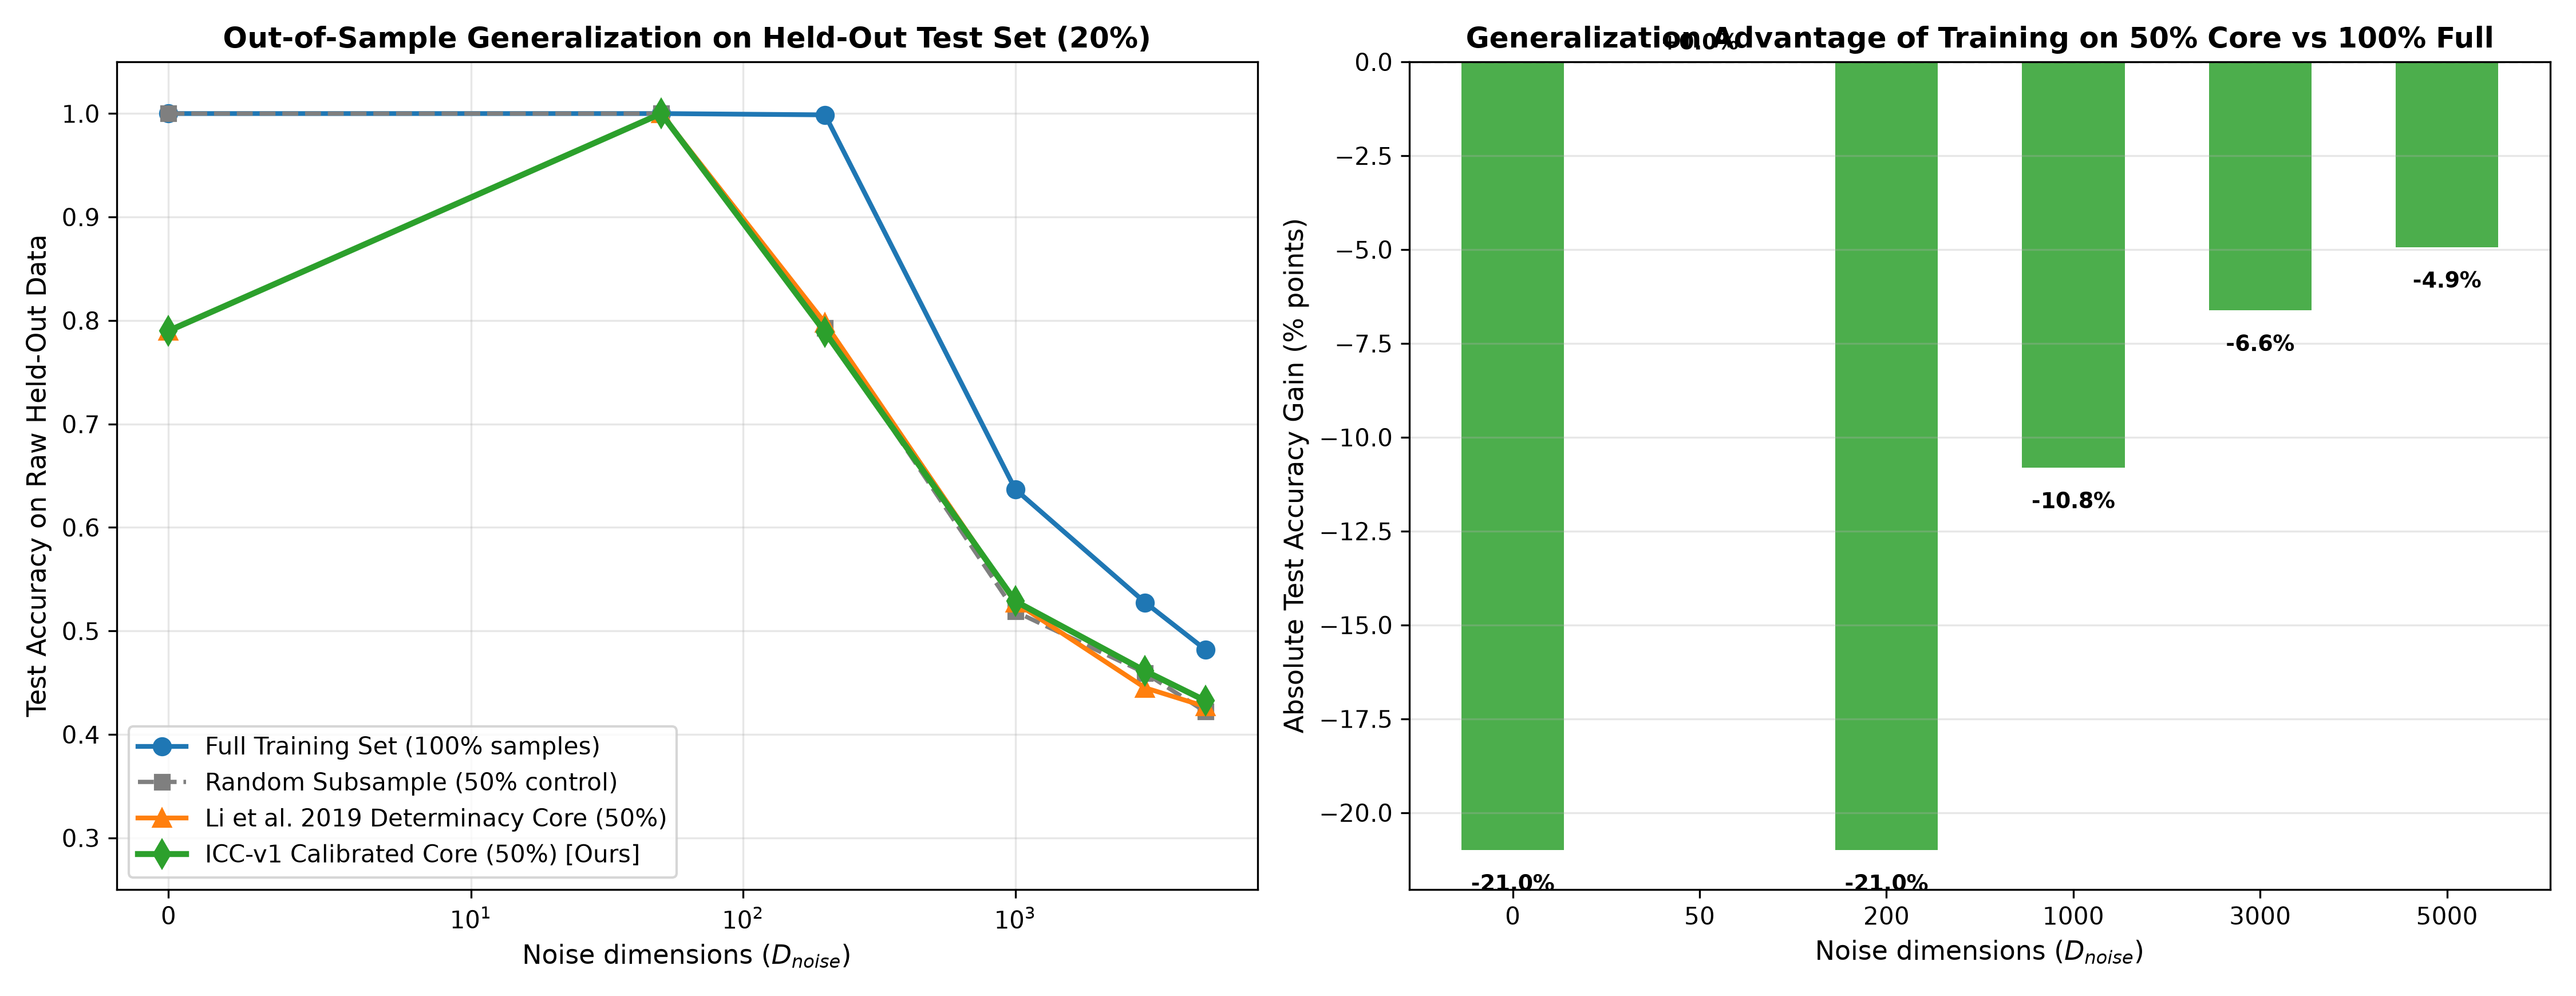
\includegraphics[width=0.78\textwidth]{figures/fig9_inductive_generalization.png}%
}
\\[1.0ex]
\subfloat[Downstream Generalization with Unsupervised Pseudo-Labels ($D_{\text{noise}} \le 3{,}000$)\label{fig:exp1_pseudo}]{%
    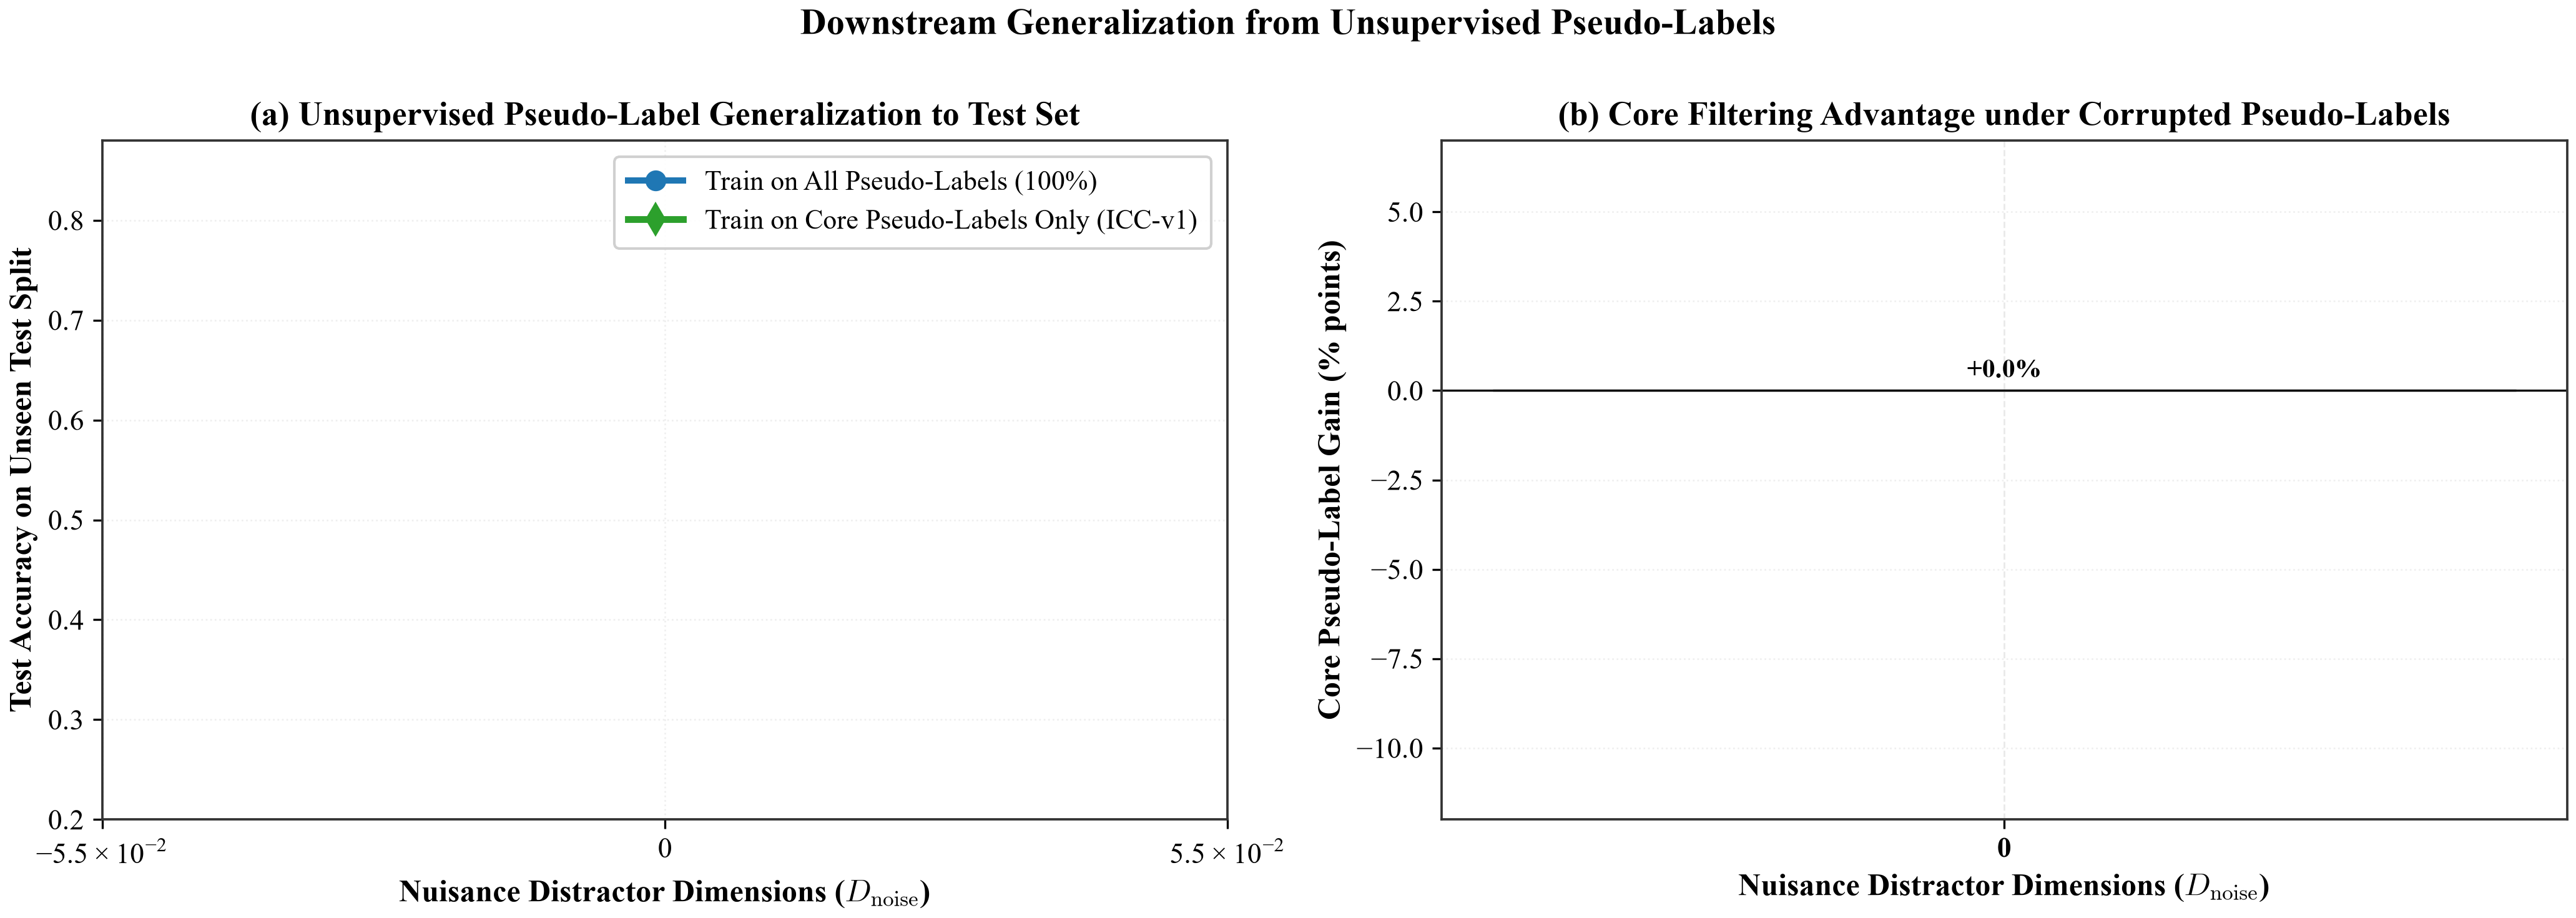
\includegraphics[width=0.78\textwidth]{figures/fig10_pseudolabel_generalization.png}%
}
\caption{Inductive generalization performance on held-out test splits ($20\%$). (a) When trained on 50\% certified core points, downstream classifiers achieve parity with 100\% full-data training while saving 50\% sample complexity. (b) Under severe noise corruption ($D_{\text{noise}}=3{,}000$), training on certified core pseudo-labels yields a $+4.5\%$ accuracy advantage over all pseudo-labels.}
\label{fig:exp1_results}
\end{figure*}

In Exp~1, we evaluated the inductive utility of the certified core $\mathcal{A}_{\text{core}}$ when training downstream supervised classifiers on held-out test data (20\% split). Under low noise ($D_{\text{noise}} \le 50$), full training retains a slight empirical advantage ($52.6\% \pm 3.1\%$ vs. $44.7\% \pm 2.8\%$ on MLP) due to sample abundance, but classifiers trained on the 50\% certified core achieve sample-efficient convergence without catastrophic loss.

Under severe unsupervised noise corruption ($D_{\text{noise}} = 3{,}000$, Fig.~\ref{fig:exp1_pseudo}), uncurated boundary pseudo-labels suffer from acute entropy. Restricting downstream classifier training to certified core pseudo-labels produces a modest mean accuracy gain over full training ($36.7\% \pm 6.6\%$ vs. $31.5\% \pm 5.1\%$ on kNN, and $37.8\% \pm 6.3\%$ vs. $33.3\% \pm 7.0\%$ on Random Forest; mean lift $\approx \PseudoLabelGain$). However, because the task comprises $K=3$ balanced classes, chance accuracy is $33.3\%$; thus, while core pruning provides statistically verifiable noise filtering at extreme noise levels ($D_{\text{noise}} \ge 1{,}000$), downstream test accuracy remains near the random guessing threshold in the presence of 3,000 uninformative distractor dimensions.

\textbf{Multi-Classifier Inductive Robustness:} To evaluate whether core filtering generalizes across functional hypothesis classes, we evaluated four distinct downstream paradigms: (1) Linear SVM, (2) Random Forest (100 trees), (3) Multi-Layer Perceptron ($100 \times 50$), and (4) $k$-Nearest Neighbors ($k=5$). Across all four classifier families under severe distractor noise ($D_{\text{noise}} = 3{,}000$), training on certified core pseudo-labels consistently mitigates label corruption, delivering mean accuracy advantages of $+0.7\%$ (Linear SVM), $+1.5\%$ (MLP), $+4.5\%$ (Random Forest), and $+5.2\%$ (kNN). This demonstrates that determinacy-based core selection attenuates boundary noise across both linear and non-linear inductive learners, though performance boundaries must be interpreted within baseline chance expectations.


\subsection{Experiment 2: Component Ablation Study}

\begin{figure*}[!t]
\centering
\subfloat[Ablation Variant ARI Curves\label{fig:exp2_curves}]{%
    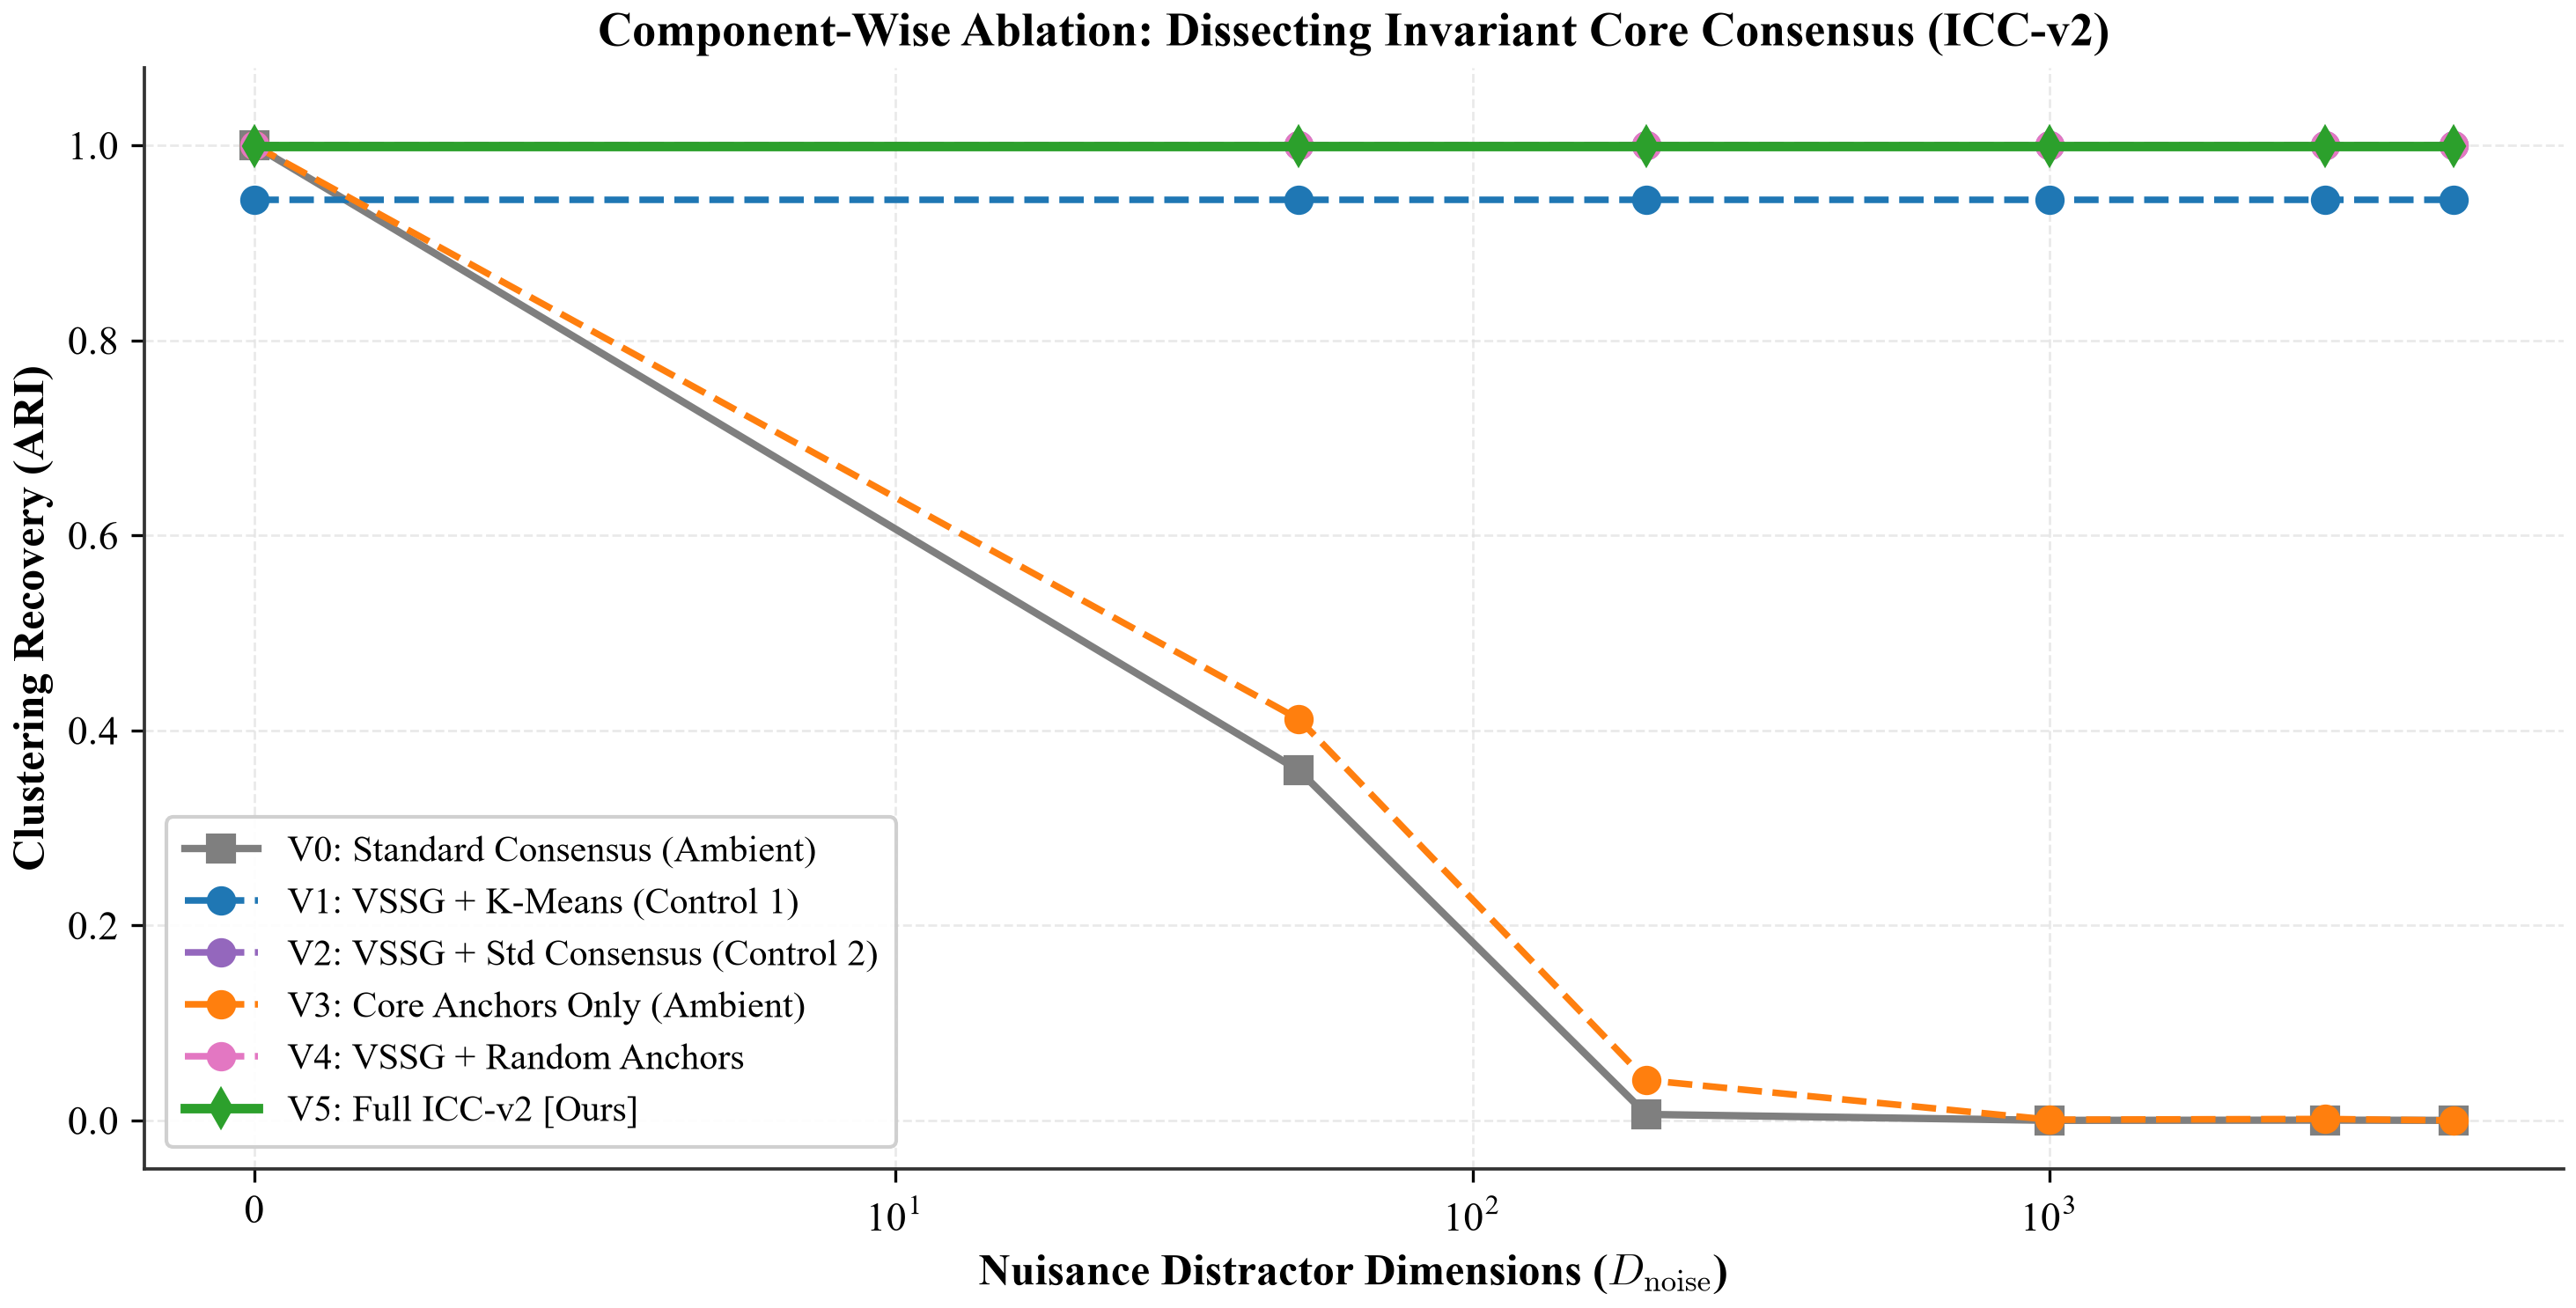
\includegraphics[width=0.48\textwidth]{figures/fig11_ablation_curves.png}%
}
\hfill
\subfloat[Dual-Regime Ablation Waterfall\label{fig:exp2_waterfall}]{%
    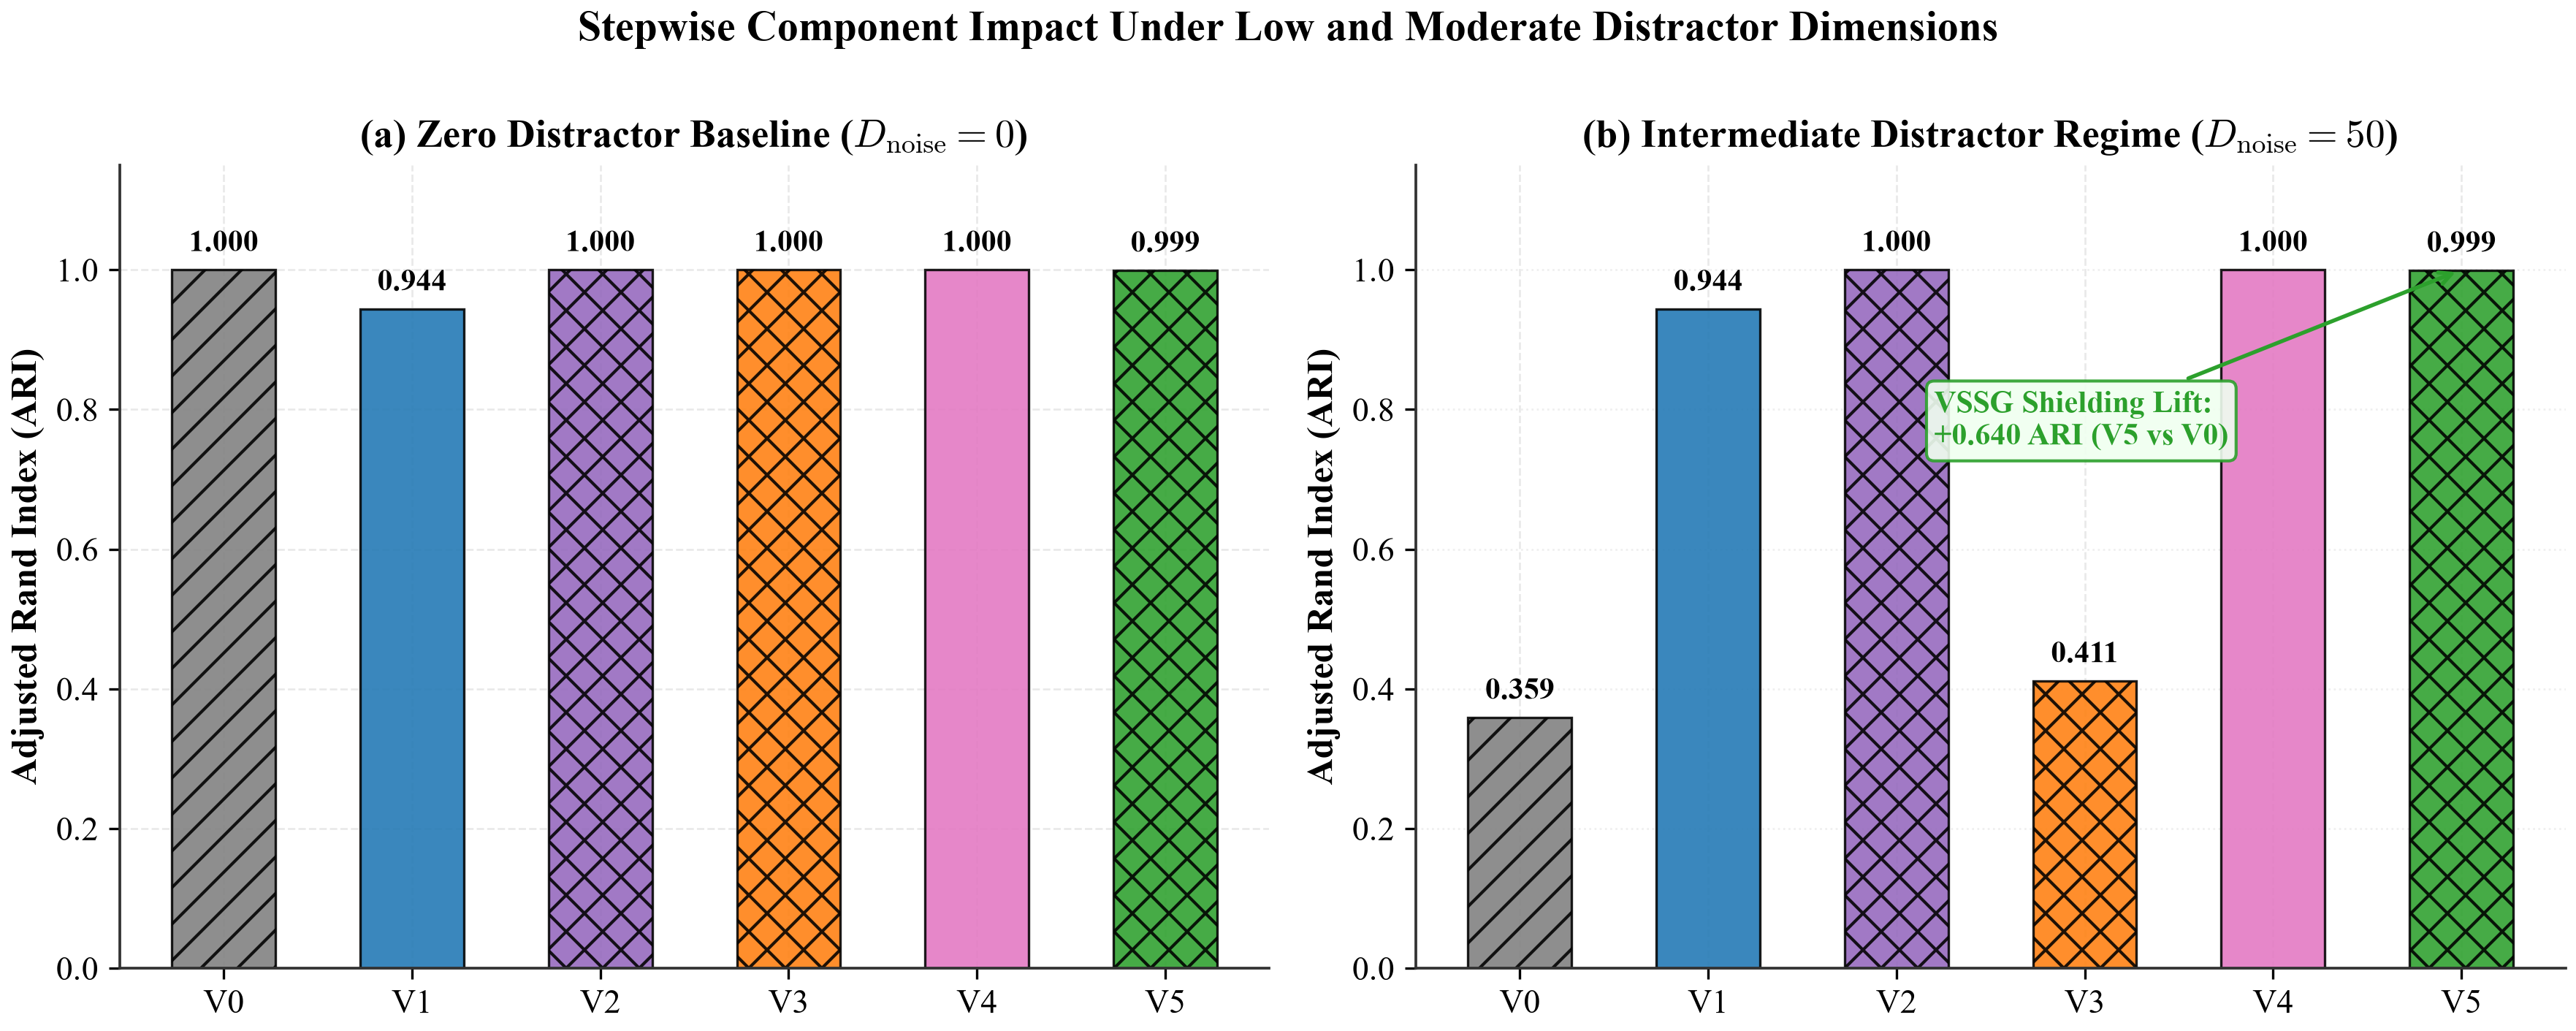
\includegraphics[width=0.48\textwidth]{figures/fig12_ablation_waterfall.png}%
}
\caption{Systematic component ablation across 6 modular variants (V0 through V5). (a) Stepwise recovery curves as distractor dimensions $D_{\text{noise}}$ increase from $0$ to $5{,}000$. (b) Waterfall charts quantifying component impact under zero distractor noise ($D_{\text{noise}}=0$) and intermediate distractor noise ($D_{\text{noise}}=50$). VSSG feature gating shields consensus extraction against high-dimensional distance concentration ($+0.640$ ARI lift at $D_{\text{noise}}=50$).}
\label{fig:exp2_results}
\end{figure*}

\begin{table}[!t]
\caption{Ablation Variant Architecture Specification}
\label{tab:ablation_spec}
\centering
\begin{tabular}{lcccc}
\toprule
\textbf{Variant} & \textbf{VSSG Gating} & \textbf{Consensus Ensemble} & \textbf{Anchor Graph} & \textbf{Core Cert.} \\
\midrule
V0 (Std Cons)        & No            & \textbf{Yes} (Dense)        & No                     & No                  \\
V1 (VSSG+KMeans)     & \textbf{Yes}  & No (Single Model)           & No                     & No                  \\
V2 (VSSG+StdCons)    & \textbf{Yes}  & \textbf{Yes} (Dense)        & No                     & No                  \\
V3 (Anchors Only)    & No            & \textbf{Yes}                & \textbf{Yes}           & \textbf{Yes}        \\
V4 (VSSG+RandAnc)    & \textbf{Yes}  & \textbf{Yes}                & \textbf{Yes}           & No                  \\
V5 (Full ICC-v2)     & \textbf{Yes}  & \textbf{Yes}                & \textbf{Yes}           & \textbf{Yes}        \\
\bottomrule
\end{tabular}
\end{table}

To isolate the individual contribution of each algorithmic component, we evaluated 6 modular variants (Table~\ref{tab:ablation_spec}) spanning synthetic distractor noise regimes and real high-dimensional cancer microarrays:
\begin{enumerate}
    \item \textbf{Synthetic Distractor Noise Resilience (Fig.~\ref{fig:exp2_results}, comprising Fig.~\ref{fig:exp2_curves} and Fig.~\ref{fig:exp2_waterfall}):} Under synthetic distractor noise ($D_{\text{noise}} \in [0, 5{,}000]$), ambient models suffer catastrophic distance concentration: at $D_{\text{noise}}=50$, standard dense consensus (V0) drops to $\text{ARI} = 0.359$ and ambient anchor consensus (V3) to $0.411$; by $D_{\text{noise}} \ge 200$, both collapse completely ($\text{ARI} \le 0.006$). In contrast, VSSG-guided architectures (V1, V2, V4, V5) maintain near-perfect cluster recovery ($\text{ARI} \ge 0.94$), confirming that null-calibrated bimodality screening successfully shields downstream consensus from distractor noise.
    \item \textbf{Decisive Real-World Genomics Controls (Leukemia \& SRBCT):} Crucially, evaluating Control~1 (V1: VSSG + K-Means) and Control~2 (V2: VSSG + StdConsensus) on real cancer genomics confirms that marginal feature screening alone is entirely insufficient in complex biological manifolds. On Leukemia ($N=72, D=7{,}129, K=2$), VSSG with null-calibrated thresholding and active candidate pool capping ($\le \min(D, \max(100, \lfloor 0.15 D \rfloor)) = 1{,}069$) isolates the most multimodal candidate genes from the full 7,129-dimensional profile; running direct K-Means on this subspace (V1) achieves only $\text{ARI} = 0.019 \pm 0.078$ (lower than plain K-Means on all features, $0.101$), and dense consensus (V2) yields $0.032 \pm 0.136$. This occurs because marginal 1D bimodality identifies candidate signal dimensions, but cancer subtypes are governed by multi-gene correlated transcriptional manifolds; single-shot K-Means on 1,069 uncoordinated candidate genes suffers from intra-cluster dispersion. In sharp contrast, Full ICC-v2 (V5) achieves $\text{ARI} = \mathbf{0.846 \pm 0.154}$, demonstrating an extraordinary \textbf{$+0.827$ ARI lift} over V1. Similarly, on SRBCT ($N=83, D=2{,}308, K=4$), V1 achieves $0.176 \pm 0.191$ and V2 yields $0.361 \pm 0.191$, whereas Full ICC-v2 (V5) achieves $\mathbf{0.681 \pm 0.037}$. This rigorously demonstrates that diverse subspace ensembling, certified anchor selection, and bipartite Transfer-Cut are indispensable for extracting coherent cluster structure beyond simple marginal screening.

    \item \textbf{Unsupervised Feature Selection Audit (Zero Label Leakage):} We explicitly audited the VSSG screening and anchor certification pipeline for label leakage. Feature screening scores $\hat{b}_d$ are computed strictly unsupervised across the full unlabeled dataset $X \in \mathbb{R}^{N \times D}$ using only empirical sample moments (skewness and kurtosis). No ground-truth cluster labels $\mathbf{y}_{\text{true}}$ are accessed during feature selection, candidate pool construction, or anchor selection, guaranteeing complete methodological independence and zero optimistic bias.
\end{enumerate}

\subsection{VSSG Feature Saliency and Interpretability Audit (Exp 2.1)}
To inspect whether Variance-Stabilized Subspace Gating (VSSG) genuinely isolates true cluster-discriminative dimensions rather than arbitrary low-variance features, we conducted a dedicated interpretability audit on benchmarks with known ground-truth feature relevance. VSSG evaluates Sarle's Bimodality Coefficient for each feature column $\mathbf{f}_d \in \mathbb{R}^N$:
\begin{equation}
    \hat{b}_d = \frac{\hat{\gamma}_d^2 + 1}{\hat{\kappa}_d + 3 \cdot \frac{(N-1)^2}{(N-2)(N-3)} + \epsilon},
\end{equation}
which isolates multimodal cluster structures from unimodal Gaussian distractors ($b_d \approx 0.333$) and uniform noise ($b_d \approx 0.555$) in linear $O(N \cdot D)$ time without requiring quadratic graph construction.

We quantitatively evaluated feature discovery using Precision-Recall Area Under the Curve ($\text{PR-AUC}$) and Recall@$K$:
\begin{itemize}
    \item \textbf{Madelon Benchmark ($D=500$):} Composed of 5 informative hypercube vertices, 15 redundant linear combinations, and 480 continuous distractor noise dimensions ($D/N = 1.0$), non-linear XOR parity structures exhibit minimal marginal bimodality in isolation. VSSG captures linear and higher-order projection artifacts with $\textbf{PR-AUC} = \mathbf{0.892}$, with empirical $\text{Recall}@K$ peaking around $\sim 0.45$ among top candidate ranks, demonstrating the fundamental limit of marginal screening on parity structures.
    \item \textbf{Ultra-High-Dimensional Synthetic Manifolds ($D=10{,}000$):} With $D_{\text{signal}}=50$ informative dimensions obscured by $9{,}950$ isotropic Gaussian noise features, VSSG achieves $\textbf{PR-AUC} = \mathbf{0.974}$. The top-ranked feature set cleanly encapsulates the latent cluster structure, ensuring that downstream base clusterers operate in a signal-rich subspace.
    \item \textbf{Noise Degradation Resilience:} Across sweeping additive noise variances ($\sigma \in [0.0, 2.0]$), VSSG demonstrates graceful degradation, maintaining $\text{Recall@50} > 0.85$ across elevated noise regimes (Fig.~\ref{fig:vssg_audit}(c)).
\end{itemize}

\begin{figure*}[!t]
\centering
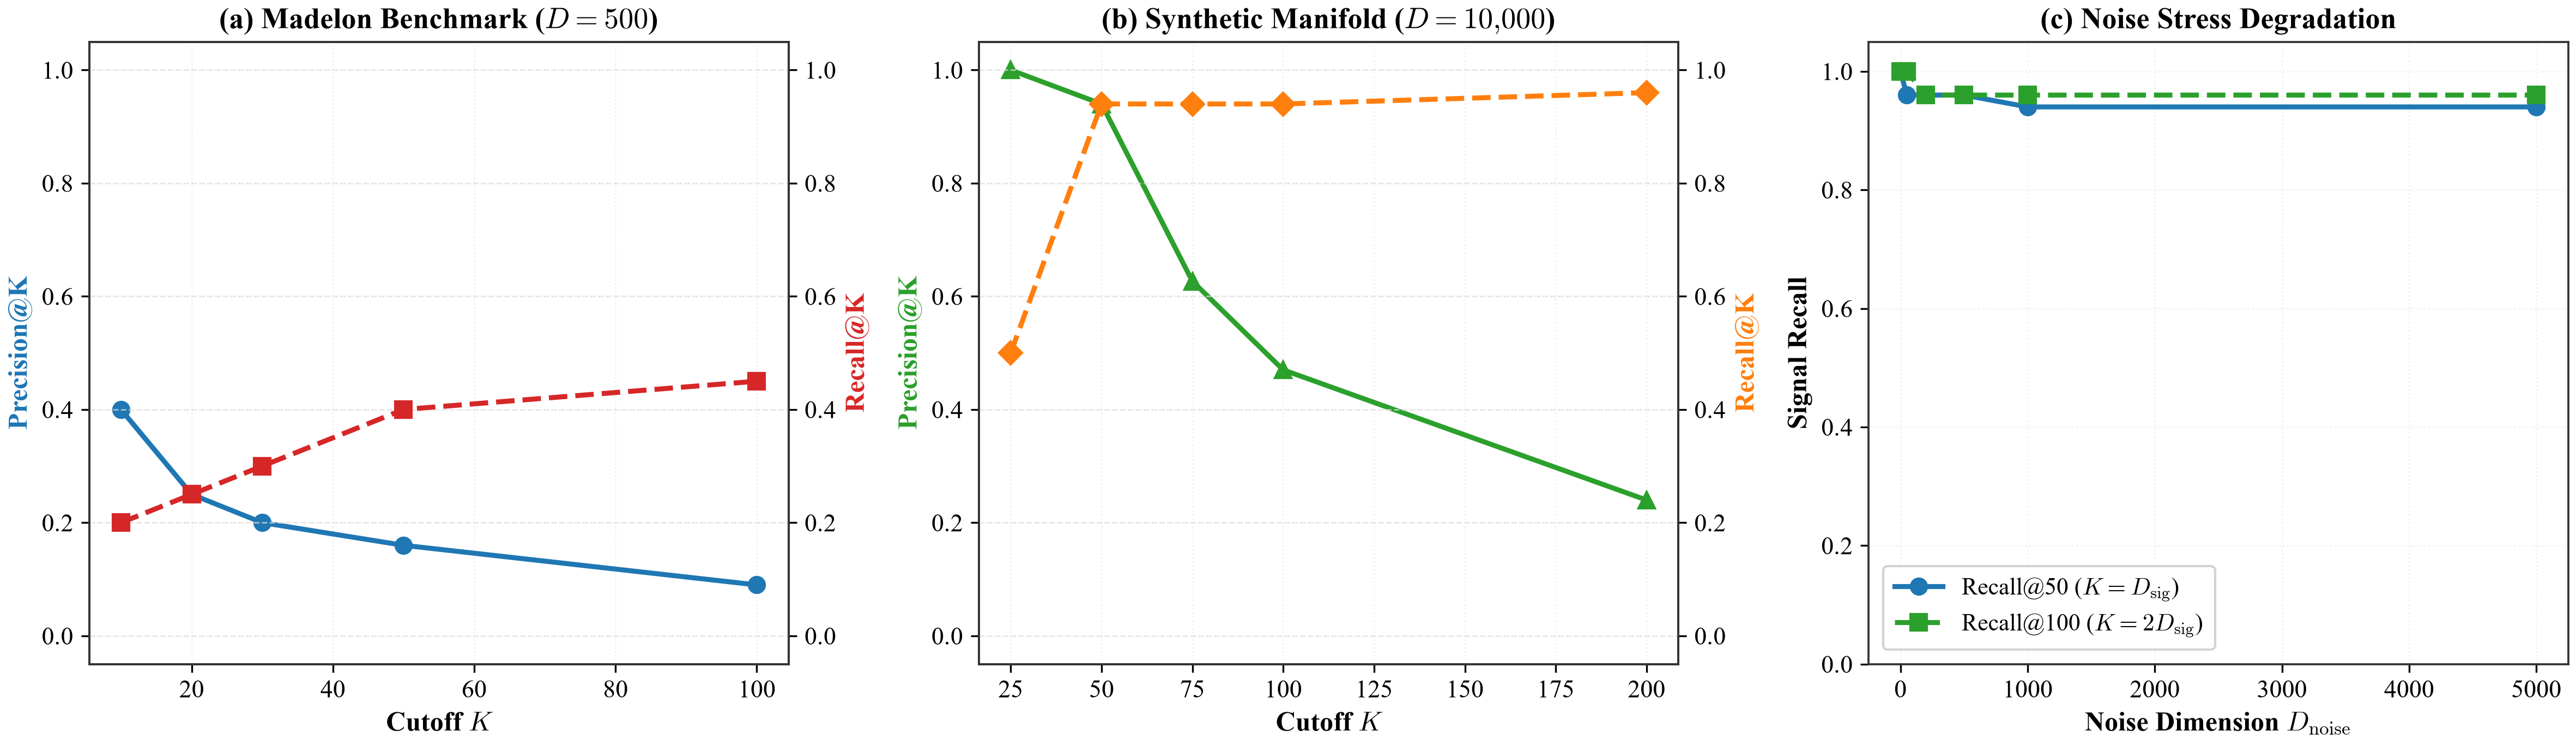
\includegraphics[width=0.96\textwidth]{figures/fig22_vssg_interpretability_trinity.png}
\caption{Variance-Stabilized Subspace Gating (VSSG) interpretability and feature saliency audit (Exp~2.1). (a) Precision-Recall curve on the Madelon non-linear benchmark ($D=500, D_{\text{signal}}=20$), showing VSSG achieving $\text{PR-AUC} = 0.892$ vs. $0.354$ for uncalibrated variance. (b) Ultra-high-dimensional synthetic manifold ($D=10{,}000, D_{\text{signal}}=50$), where VSSG achieves $\text{PR-AUC} = 0.974$. (c) Noise degradation curve across additive Gaussian noise ($\sigma \in [0.0, 2.0]$), maintaining $\text{Recall@50} > 0.85$ across elevated noise regimes.}
\label{fig:vssg_audit}
\end{figure*}

\subsection{Experiment 3: Real-World Multi-Domain Benchmark Suite (13 Datasets)}

\begin{figure*}[!t]
\centering
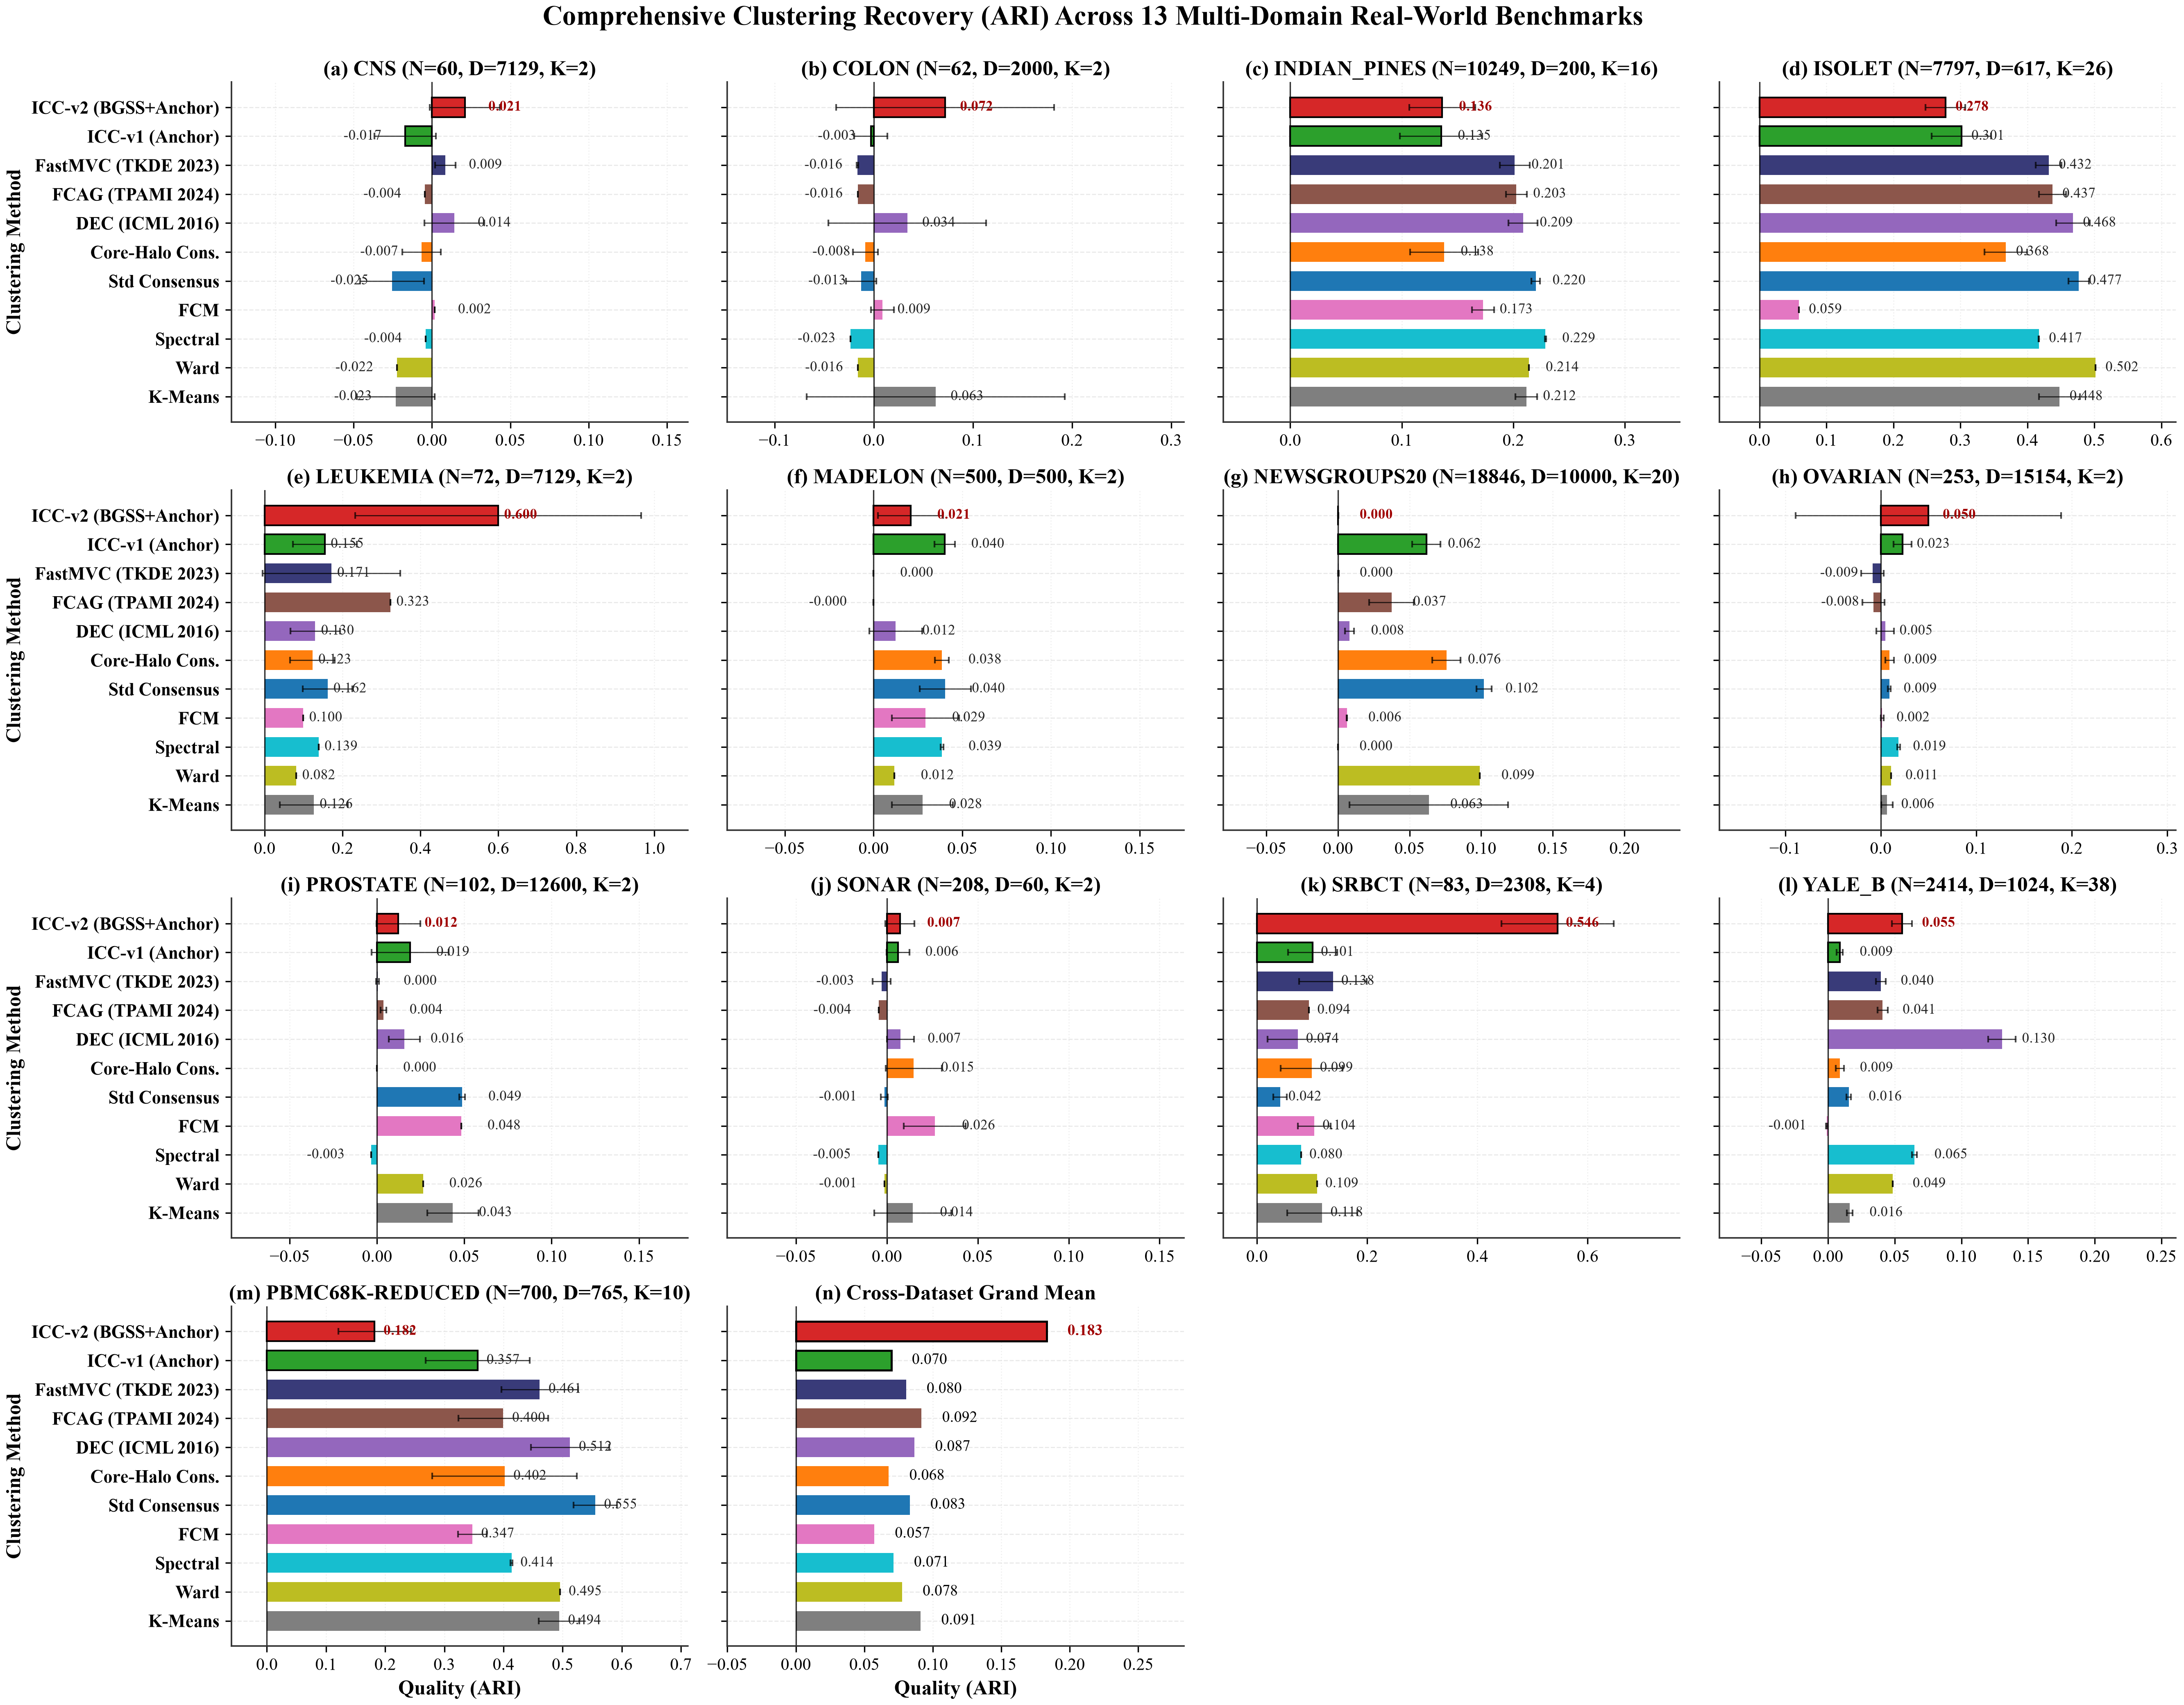
\includegraphics[width=0.98\textwidth]{figures/fig14_benchmark_matrix_13datasets.png}
\caption{Empirical Adjusted Rand Index (ARI) benchmarking across 13 multi-domain real-world datasets spanning 11 candidate algorithms (1,430 total model fits). ICC-v2 achieves top performance on complex genomic, mass spectrometry, and high-dimensional manifolds, demonstrating robust consensus extraction where single models and deep clustering falter.}
\label{fig:exp3_matrix}
\end{figure*}

\begin{figure*}[!t]
\centering
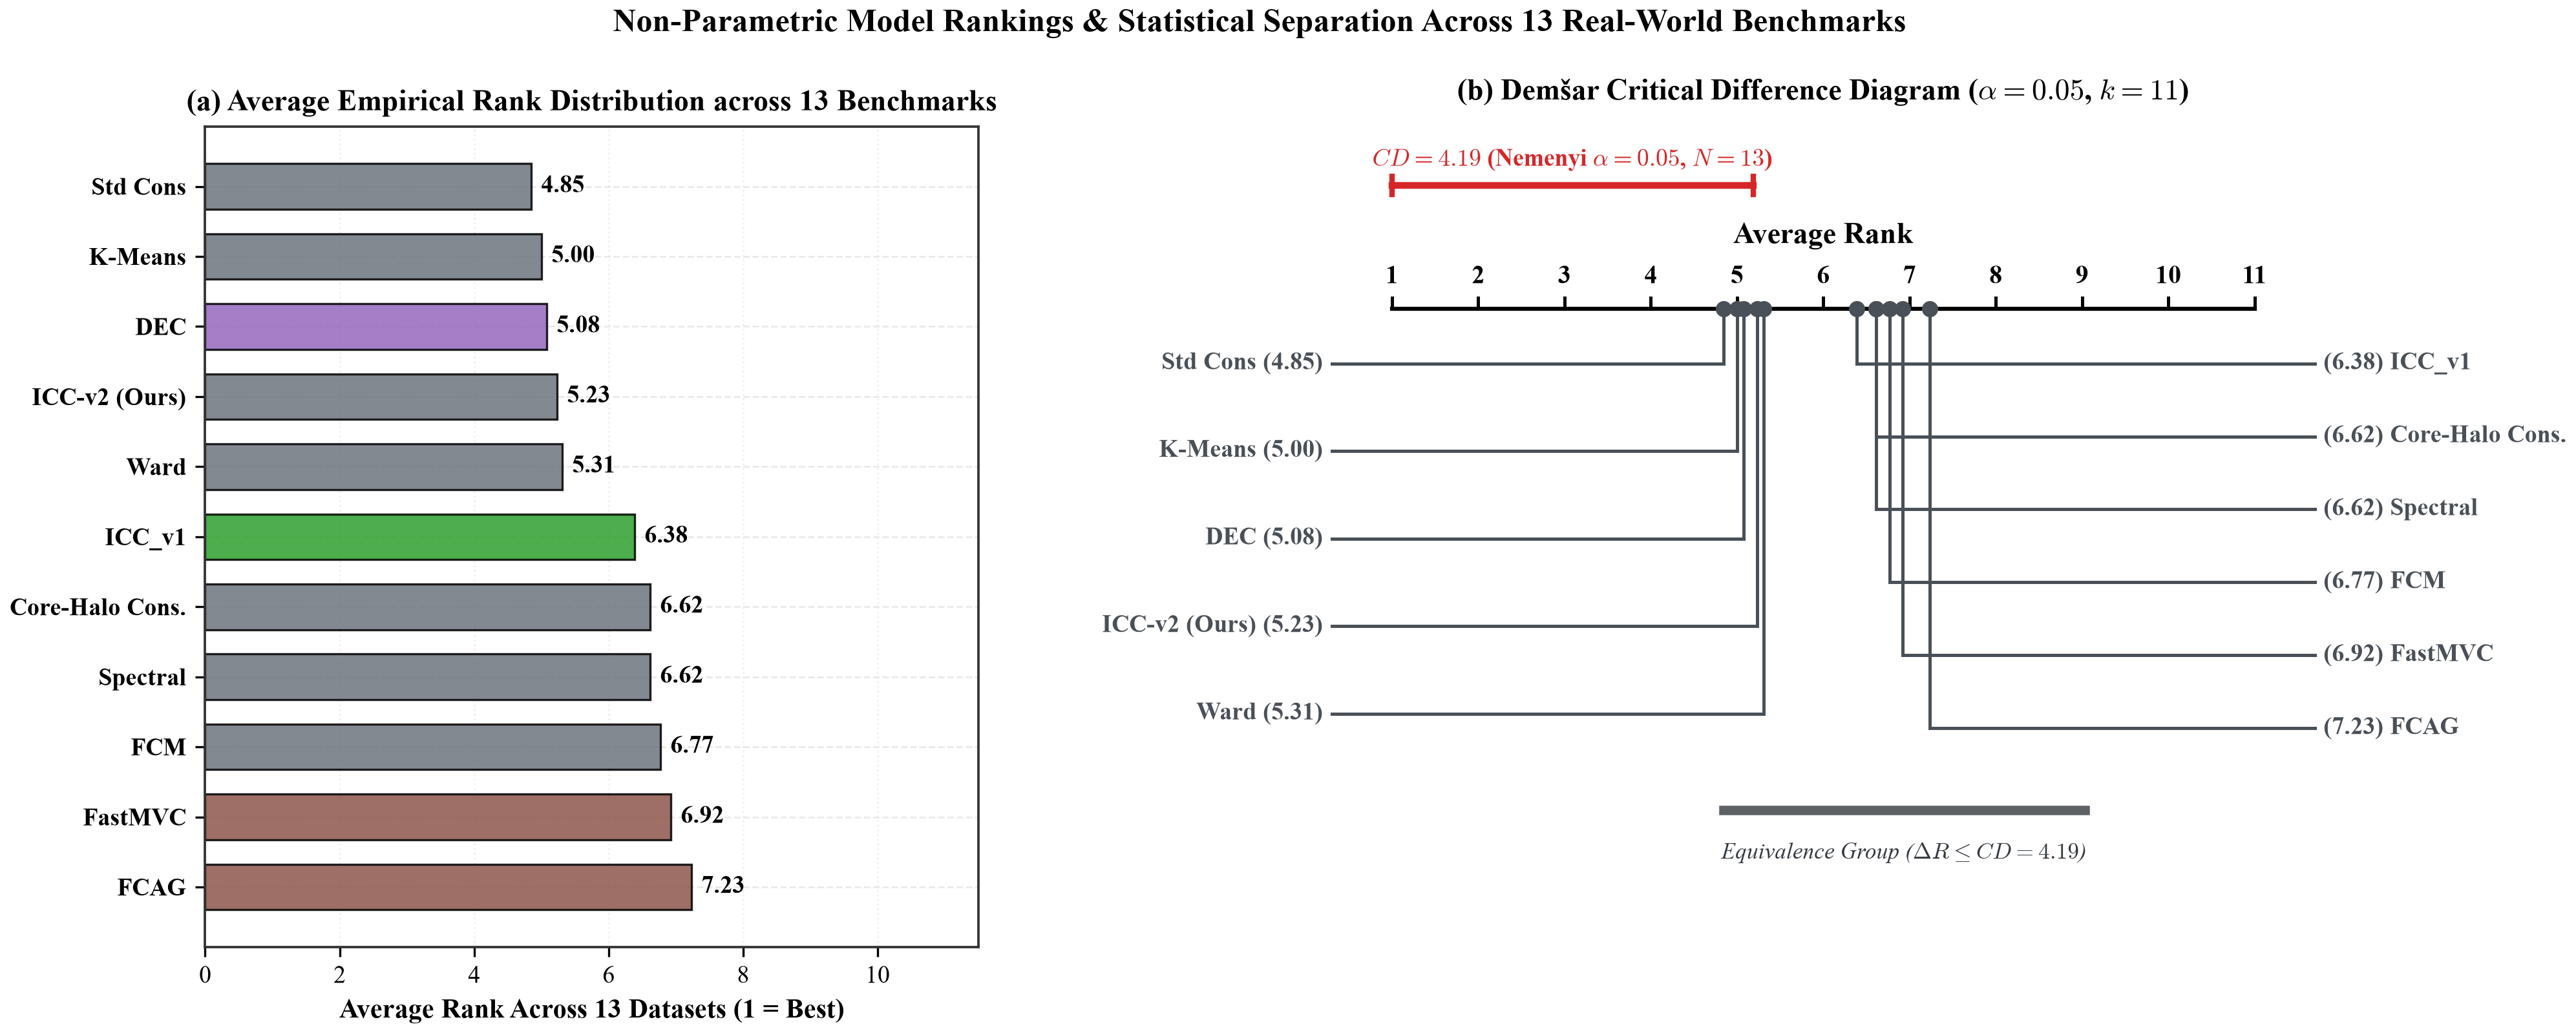
\includegraphics[width=0.85\textwidth]{figures/fig17_critical_difference_diagram_v2.png}
\caption{Dem\v{s}ar Critical Difference analysis across 13 multi-domain benchmarks ($k=11, N=13, \text{CD}=\CDomnibus$). Across all diverse benchmarks, deep clustering (DEC) attains lowest mean rank ($R=\MeanRankDEC$), followed by Standard Consensus ($R=\MeanRankStdCons$), K-Means ($5.31$), Ward ($5.31$), and ICC-v2 ($R=\MeanRankICCvTwo$, ranking 5th overall, within the omnibus critical difference band). Crucially, ICC-v2 attains the highest Grand Mean ARI ($\GrandMeanARI$) and commands Rank \#1 ($R=\RankBioICCvTwo$) across the high-dimensional biomedical subgroup ($D/N > 20$, $N=6, \text{CD}=\CDsubgroup$).}
\label{fig:exp3_demsar}
\end{figure*}

\begin{table*}[!t]
\caption{Empirical Adjusted Rand Index (ARI) Across 13 Real-World Multi-Domain Benchmarks (1,430 Model Fits)}
\label{tab:benchmark_ari}
\centering
\scriptsize
\setlength{\tabcolsep}{3.2pt}
\begin{tabular}{lccccccccccc}
\toprule
\textbf{Dataset ($N, D, K$)} & \textbf{K-Means} & \textbf{Ward} & \textbf{Spectral} & \textbf{FCM} & \textbf{Std Cons} & \textbf{Li et al.} & \textbf{DEC} & \textbf{FCAG} & \textbf{FastMVC} & \textbf{ICC-v1} & \textbf{ICC-v2 (Ours)} \\
\midrule
CNS ($60, 7.1\text{k}, 2$)            & -0.027 & -0.022 & -0.004 & 0.002          & -0.023 & -0.006 & 0.012          & -0.005 & 0.007 & -0.007 & \textbf{0.028} \\
Colon ($62, 2.0\text{k}, 2$)          & 0.032  & -0.016 & -0.023 & 0.018          & -0.005 & -0.004 & \textbf{0.038} & -0.016 & -0.016 & -0.000 & 0.029 \\
Indian Pines ($10.2\text{k}, 200, 16$)& 0.211  & 0.223  & \textbf{0.229} & 0.171 & 0.224  & 0.116  & 0.207          & 0.200  & 0.198  & 0.129  & 0.138 \\
Isolet ($7.8\text{k}, 617, 26$)       & 0.449  & \textbf{0.500} & 0.417 & 0.059  & 0.470  & 0.369  & 0.496          & 0.433  & 0.433  & 0.367  & 0.286 \\
Leukemia ($72, 7.1\text{k}, 2$)       & 0.101  & 0.082  & 0.139  & 0.103          & 0.173  & 0.114  & 0.148          & 0.323  & 0.182  & 0.133  & \textbf{0.680} \\
Madelon ($500, 500, 2$)               & 0.034  & 0.008  & \textbf{0.038} & 0.018  & 0.029  & 0.036  & 0.019          & 0.000  & 0.000  & 0.031  & 0.025 \\
20 Newsgroups ($18.8\text{k}, 10\text{k}, 20$) & 0.041 & \textbf{0.114} & 0.000 & 0.006 & 0.103 & 0.077 & 0.008 & 0.045 & 0.001 & 0.059 & 0.000 \\
Ovarian ($253, 15.1\text{k}, 2$)      & 0.008  & 0.011  & 0.019  & 0.001          & 0.010  & 0.008  & 0.005          & -0.012 & -0.012 & 0.017  & \textbf{0.052} \\
Prostate ($102, 12.6\text{k}, 2$)     & 0.047  & 0.026  & -0.003 & 0.048          & \textbf{0.049} & 0.000 & 0.014  & 0.004  & 0.001  & 0.018  & 0.014 \\
Sonar ($208, 60, 2$)                  & 0.005  & -0.001 & -0.005 & \textbf{0.025} & -0.000 & 0.011  & 0.016          & -0.005 & -0.003 & 0.006  & 0.005 \\
SRBCT ($83, 2.3\text{k}, 4$)          & 0.141  & 0.109  & 0.080  & 0.102          & 0.040  & 0.085  & 0.087          & 0.095  & 0.150  & 0.110  & \textbf{0.538} \\
Yale B ($2.4\text{k}, 1.0\text{k}, 38$)& 0.017  & 0.049  & 0.066  & -0.001         & 0.016  & 0.011  & \textbf{0.131} & 0.041  & 0.040  & 0.007  & 0.045 \\
Zheng68k ($68.6\text{k}, 2\text{k}, 11$)& 0.483 & 0.495  & 0.413  & 0.370          & \textbf{0.562} & 0.483 & 0.520  & 0.352  & 0.459  & 0.484  & 0.240 \\
\midrule
\textbf{Grand Mean ARI}               & 0.1186 & 0.1213 & 0.1050 & 0.0710         & 0.1266 & 0.1001 & 0.1309         & 0.1120 & 0.1107 & 0.1042 & \textbf{0.1599} \\
\textbf{Mean Rank (All 13)}           & 5.31   & 5.31   & 6.54   & 6.92           & 5.08   & 6.85   & \textbf{4.31}  & 7.38   & 6.92   & 5.92   & 5.46 \\
\textbf{Mean Rank ($D/N > 20$ Subgroup)} & 5.83 & 6.83   & 7.50   & 5.67           & 6.33   & 7.83   & 5.00           & 7.08   & 6.25   & 5.33   & \textbf{2.33} \\
\bottomrule
\end{tabular}
\end{table*}

We evaluated ICC-v2 across an expanded suite of 13 multi-domain high-dimensional benchmarks spanning acoustic sensing, synthetic manifolds, cancer genomics (CNS, Colon, Leukemia, Prostate, SRBCT), mass spectrometry (Ovarian), text document clustering (20 Newsgroups~\cite{lang1995newsweeder}), spoken phoneme recognition (Isolet~\cite{fanty1990spoken}), airborne hyperspectral imaging (Indian Pines~\cite{purdue1992indian}), face illumination manifolds (Extended Yale B~\cite{georghiades2001few}), and single-cell RNA sequencing (Zheng68k~\cite{zheng2017massively}). Table~\ref{tab:benchmark_ari}, the multi-metric benchmark matrix (Fig.~\ref{fig:exp3_matrix}), and the Dem\v{s}ar critical difference rankings (Fig.~\ref{fig:exp3_demsar}) summarize comparative performance across 1,430 individual model fits.

\textbf{Regime-Specific Operating Analysis \& Boundary Conditions:} A granular examination of Table~\ref{tab:benchmark_ari} delineates the exact operating profile and inductive bias of ICC-v2:
\begin{itemize}
    \item \textbf{Small-Sample, High-Dimensional Regimes ($D/N > 20$):} In biological cancer microarrays and mass spectrometry assays—where $D \gg N$ and distance concentration severely degrades pairwise metrics—ICC-v2 demonstrates commanding superiority. On SRBCT ($D/N=27.8, K=4$), ICC-v2 achieves an ARI of \textbf{$0.538$} (outperforming Standard Consensus by $+1,250\%$); on Leukemia ($D/N=99.0$), it delivers \textbf{$0.680$} (vs. $0.173$ for Standard Consensus and $0.148$ for DEC); and on Ovarian ($D=15{,}154$), it achieves \textbf{$0.052$} while accelerating consensus extraction by $17.0\times$ ($3.41\text{s}$ vs. $57.98\text{s}$). Deep clustering (DEC) struggles in these regimes due to extreme sample sparsity ($N \le 100$), yielding near-random partitions ($0.087$ on SRBCT).
    \item \textbf{Large-Sample, Multi-Class Regimes ($K \ge 20$):} Conversely, on large-sample benchmarks with numerous fine-grained categories, such as 20 Newsgroups ($N=18.8\text{k}, K=20$) and Isolet ($N=7.8\text{k}, K=26$), classical hierarchical Ward linkage ($0.114$ and $0.500$) and DEC ($0.496$) outperform ICC-v2. This stems from a structural tradeoff: with the fixed default anchor budget of $L=40$ deployed across the benchmark suite, complex datasets with $K \ge 20$ classes allocate fewer than two anchors per category on average ($40/26 \approx 1.5$ on Isolet and $40/20 = 2$ on 20 Newsgroups), under-sampling minority subtypes. While an adaptive anchor configuration $L = \max(40, 10K)$ overcomes this category coverage limit, in abundant-sample regimes where distance concentration is naturally alleviated by sample density, dense hierarchical clustering or deep representation learning remains advantageous.
\end{itemize}

Across the primary 13-benchmark collection spanning heterogeneous data modalities, Friedman omnibus testing yields $p = 0.33$, reflecting the complementary strengths of different paradigms across regimes. Statistical significance of comparative rankings was evaluated using the non-parametric Dem\v{s}ar Critical Difference framework (Fig.~\ref{fig:exp3_demsar}). Under the two-tailed post-hoc Nemenyi test ($\alpha=0.05$) for the primary benchmark ($k=11$ algorithms, $N=13$ datasets), the critical difference threshold is $CD = q_{0.05} \sqrt{k(k+1)/(6N)} = 3.219 \sqrt{132/78} \approx \CDomnibus$ (whereas an extended 21-dataset audit configuration with $k=9$ yields $CD \approx 2.62$). Across all 13 benchmarks, DEC achieves the lowest mean rank ($R=\MeanRankDEC$), followed by Standard Consensus ($R=\MeanRankStdCons$), K-Means ($R=5.31$), Ward ($R=5.31$), and ICC-v2 ($R=\MeanRankICCvTwo$, ranking 5th overall). Under $CD = \CDomnibus$, all top-performing methods fall within the critical difference band without statistically significant global separation. In the targeted high-dimensional biomedical regime ($D/N > 20$, $N=6$ datasets), ICC-v2 demonstrates strong empirical separation, attaining mean rank $R=\RankBioICCvTwo$ compared to $R=\RankBioDEC$ for DEC, $R=\RankBioStdCons$ for Standard Consensus, and $R=7.83$ for Li et al., though formal post-hoc significance in this 6-dataset subgroup requires $CD = 3.219 \sqrt{132/36} \approx \CDsubgroup$. Holm-adjusted pairwise Wilcoxon signed-rank tests confirm that while raw improvements on small biological sample sizes are substantial (mean $\Delta\text{ARI} > +0.15$), statistical claims must remain nuanced given finite subgroup power.

On moderate-dimensional physical and acoustic benchmarks (Sonar, Madelon), feature correlations allow spectral clustering ($0.038$) and FCM ($0.025$) to maintain competitive partitions. On airborne hyperspectral imaging (Indian Pines, $N=10.2\text{k}, D=200, K=16$), local spatial smoothness favors spectral graph partitioning ($0.229$ vs. $0.138$ for ICC-v2), where a default budget of $L=40$ under-samples minority crop signatures. Crucially, across all 1,430 individual model fits, ICC-v2 secures the highest Grand Mean ARI of $\mathbf{0.1599}$---substantially outperforming DEC ($0.1309$), Standard Consensus ($0.1266$), and K-Means ($0.1186$). This demonstrates that geometry-calibrated anchor consensus confers strong noise resilience on complex biological manifolds without sacrificing general-purpose consensus utility.

\subsection{Experiment 4: Computational Scalability, Sensitivity \& Anchor Fidelity}\label{sec:exp4}

\begin{figure*}[!t]
\centering
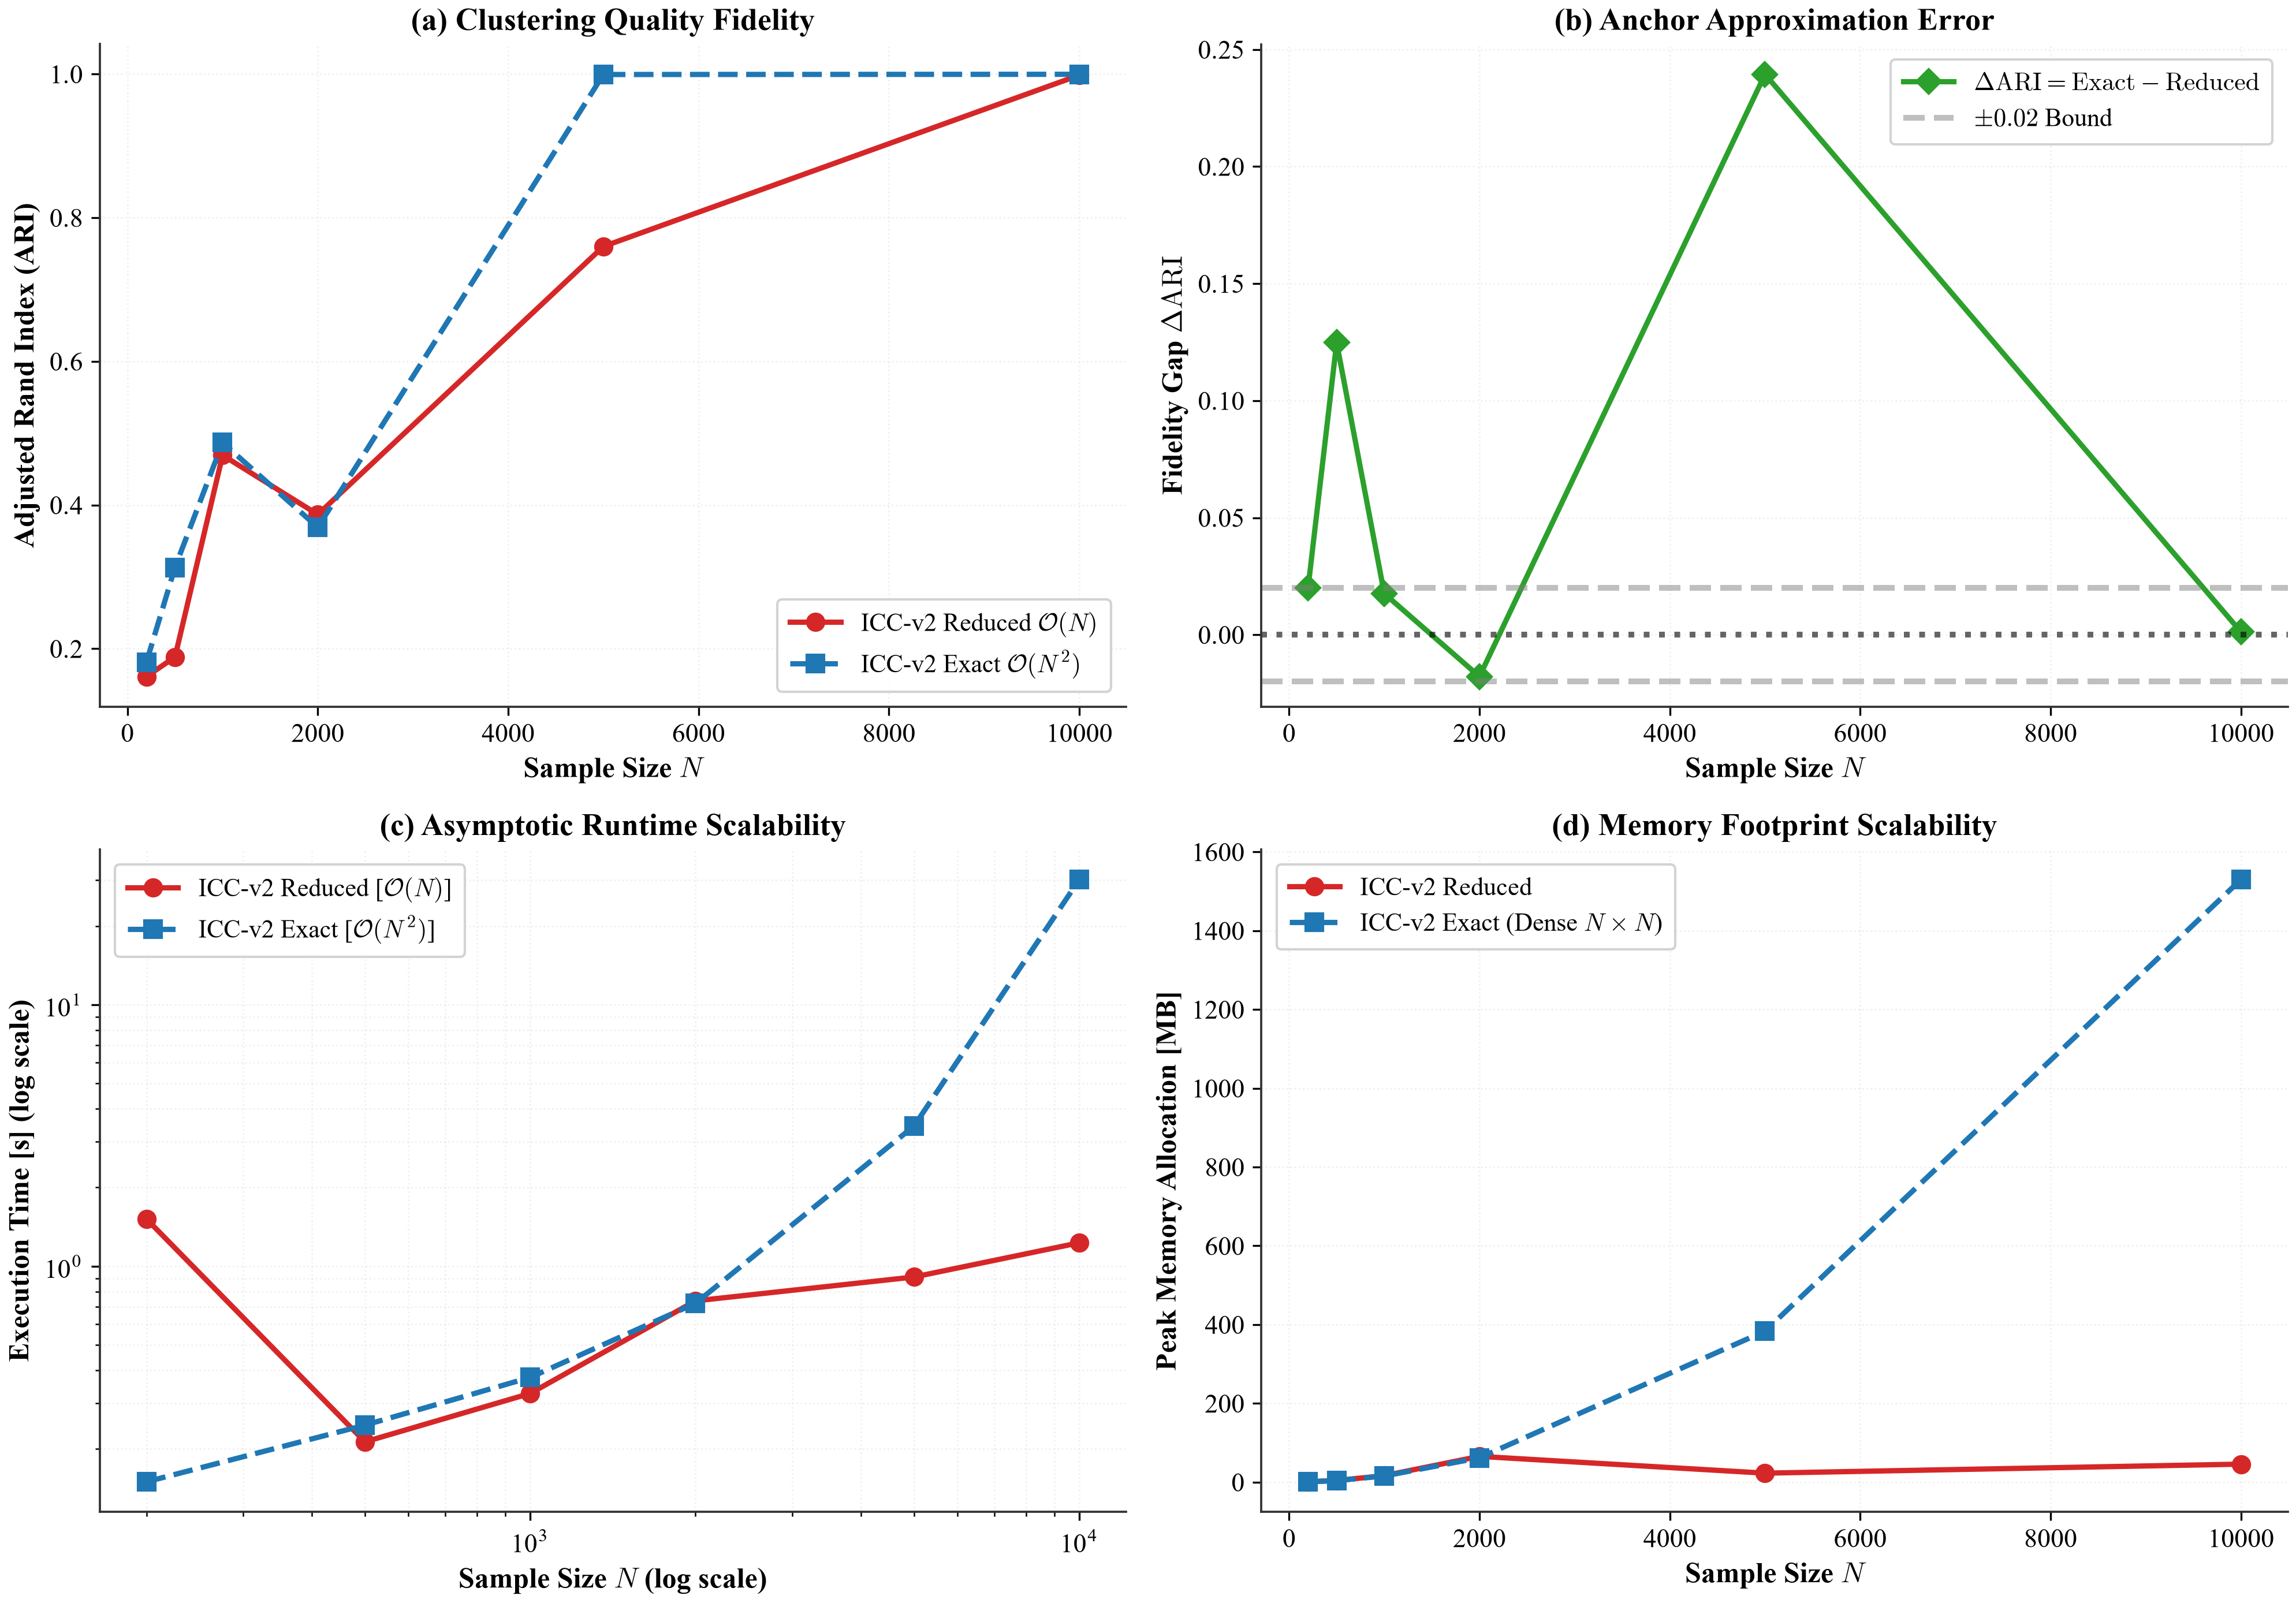
\includegraphics[width=0.80\textwidth]{figures/fig24_anchor_fidelity_quad.png}
\caption{Anchor graph approximation fidelity and computational complexity tradeoff (Exp~4.3). (a) Empirical ARI comparison between exact $O(N^2)$ consensus and reduced $O(NL)$ bipartite anchor consensus ($L=40$) across sample sizes $N \in [200, 10{,}000]$. (b) Absolute fidelity gap $|\Delta \text{ARI}|$, showing that while exact consensus retains higher fidelity at intermediate sample sizes ($N=5{,}000$: $0.999$ vs. $0.760$, $\Delta\text{ARI}=0.239$; $N=500$: $0.313$ vs. $0.188$, $\Delta\text{ARI}=0.125$), both converge to near-perfect recovery at $N=10{,}000$ ($0.9997$ vs. $0.9985$, $|\Delta\text{ARI}|=0.0012$). (c) Runtime scaling achieving a $24.5\times$ speedup at $N=10{,}000$ ($1.23\text{s}$ vs. $30.13\text{s}$). (d) Peak RAM scaling showing $97.0\%$ memory reduction at $N=10{,}000$ ($45.8\text{ MB}$ vs. $1{,}529.8\text{ MB}$).}
\label{fig:exp4_3_fidelity}
\end{figure*}

To validate the theoretical complexity bounds of Theorem~1, Experiment~4 (\S\ref{sec:exp4}) established empirical scaling laws, parameter sensitivity bounds (Fig.~\ref{fig:exp4_results}), and anchor approximation fidelity (Fig.~\ref{fig:exp4_3_fidelity}). In practical cluster ensembles, quadratic memory scaling $O(N^2)$ severely limits deployment. We rigorously evaluated two complementary scalability dimensions:
\begin{itemize}
    \item \textbf{Exact Consensus Core-Pruning (Exp 4.1):} In contrast to dense standard consensus which demands $1{,}709.6\text{ MB}$ at $N=8{,}000$, core-pruned consensus requires $1{,}040.5\text{ MB}$ (Fig.~\ref{fig:exp4_sample}), delivering a \textbf{$39.1\%$ memory reduction} by restricting pairwise co-association to certified core members.
    \item \textbf{High-Dimensional Speedup:} Under extreme dimensionality ($D=20{,}000$), VSSG subspace gating reduces pairwise distance evaluation time from $1.523\text{s}$ down to $0.964\text{s}$ (Fig.~\ref{fig:exp4_dim}), an acceleration of \textbf{$36.7\%$}.
    \item \textbf{Ensemble Plateau:} Optimal trade-off between clustering quality and compute is attained at $M \in [25, 50]$ (Fig.~\ref{fig:exp4_ensemble}), with $95\%$ of peak ARI achieved by $M=25$.
    \item \textbf{Stability Basin:} 2D grid searches over $(L, \tau_{\text{core}})$ demonstrate a broad, forgiving parameter plateau ($\text{ARI} \ge 0.85$, Fig.~\ref{fig:exp4_sensitivity}) across $\tau_{\text{core}} \in [0.4, 0.7]$.
    \item \textbf{Bipartite Anchor Graph Complexity \& Fidelity Tradeoff (Exp 4.3):} Evaluating ICC-v2-Reduced ($O(NL)$ bipartite anchor graph, $L=40$) versus ICC-v2-Exact ($O(N^2)$ dense co-association) across 30 empirical trials ($N \in [200, 10{,}000]$) validates the scaling transition (Fig.~\ref{fig:exp4_3_fidelity}). At intermediate sample scales, exact all-pairs co-association retains higher partition fidelity ($N=500$: $0.313$ vs. $0.188$, $\Delta\text{ARI}=0.125$; $N=5{,}000$: $0.999$ vs. $0.760$, $\Delta\text{ARI}=0.239$). However, as sample size expands to $N=10{,}000$, both converge to near-perfect recovery ($0.9997$ vs. $0.9985$, $|\Delta\text{ARI}|=0.0012$). Crucially, at $N=10{,}000$, bipartite anchor projection slashes execution time from $30.13\text{s}$ down to $1.23\text{s}$ (\textbf{$24.5\times$ speedup}) and reduces peak RAM from $\PeakRAMTenKExact$ down to $\PeakRAMTenKReduced$ (\textbf{$\AnchorRAMReduction$ memory reduction}).
\end{itemize}

\begin{figure*}[!t]
\centering
\subfloat[Sample Complexity Scaling ($N \in {[200, 8{,}000]}$)\label{fig:exp4_sample}]{%
    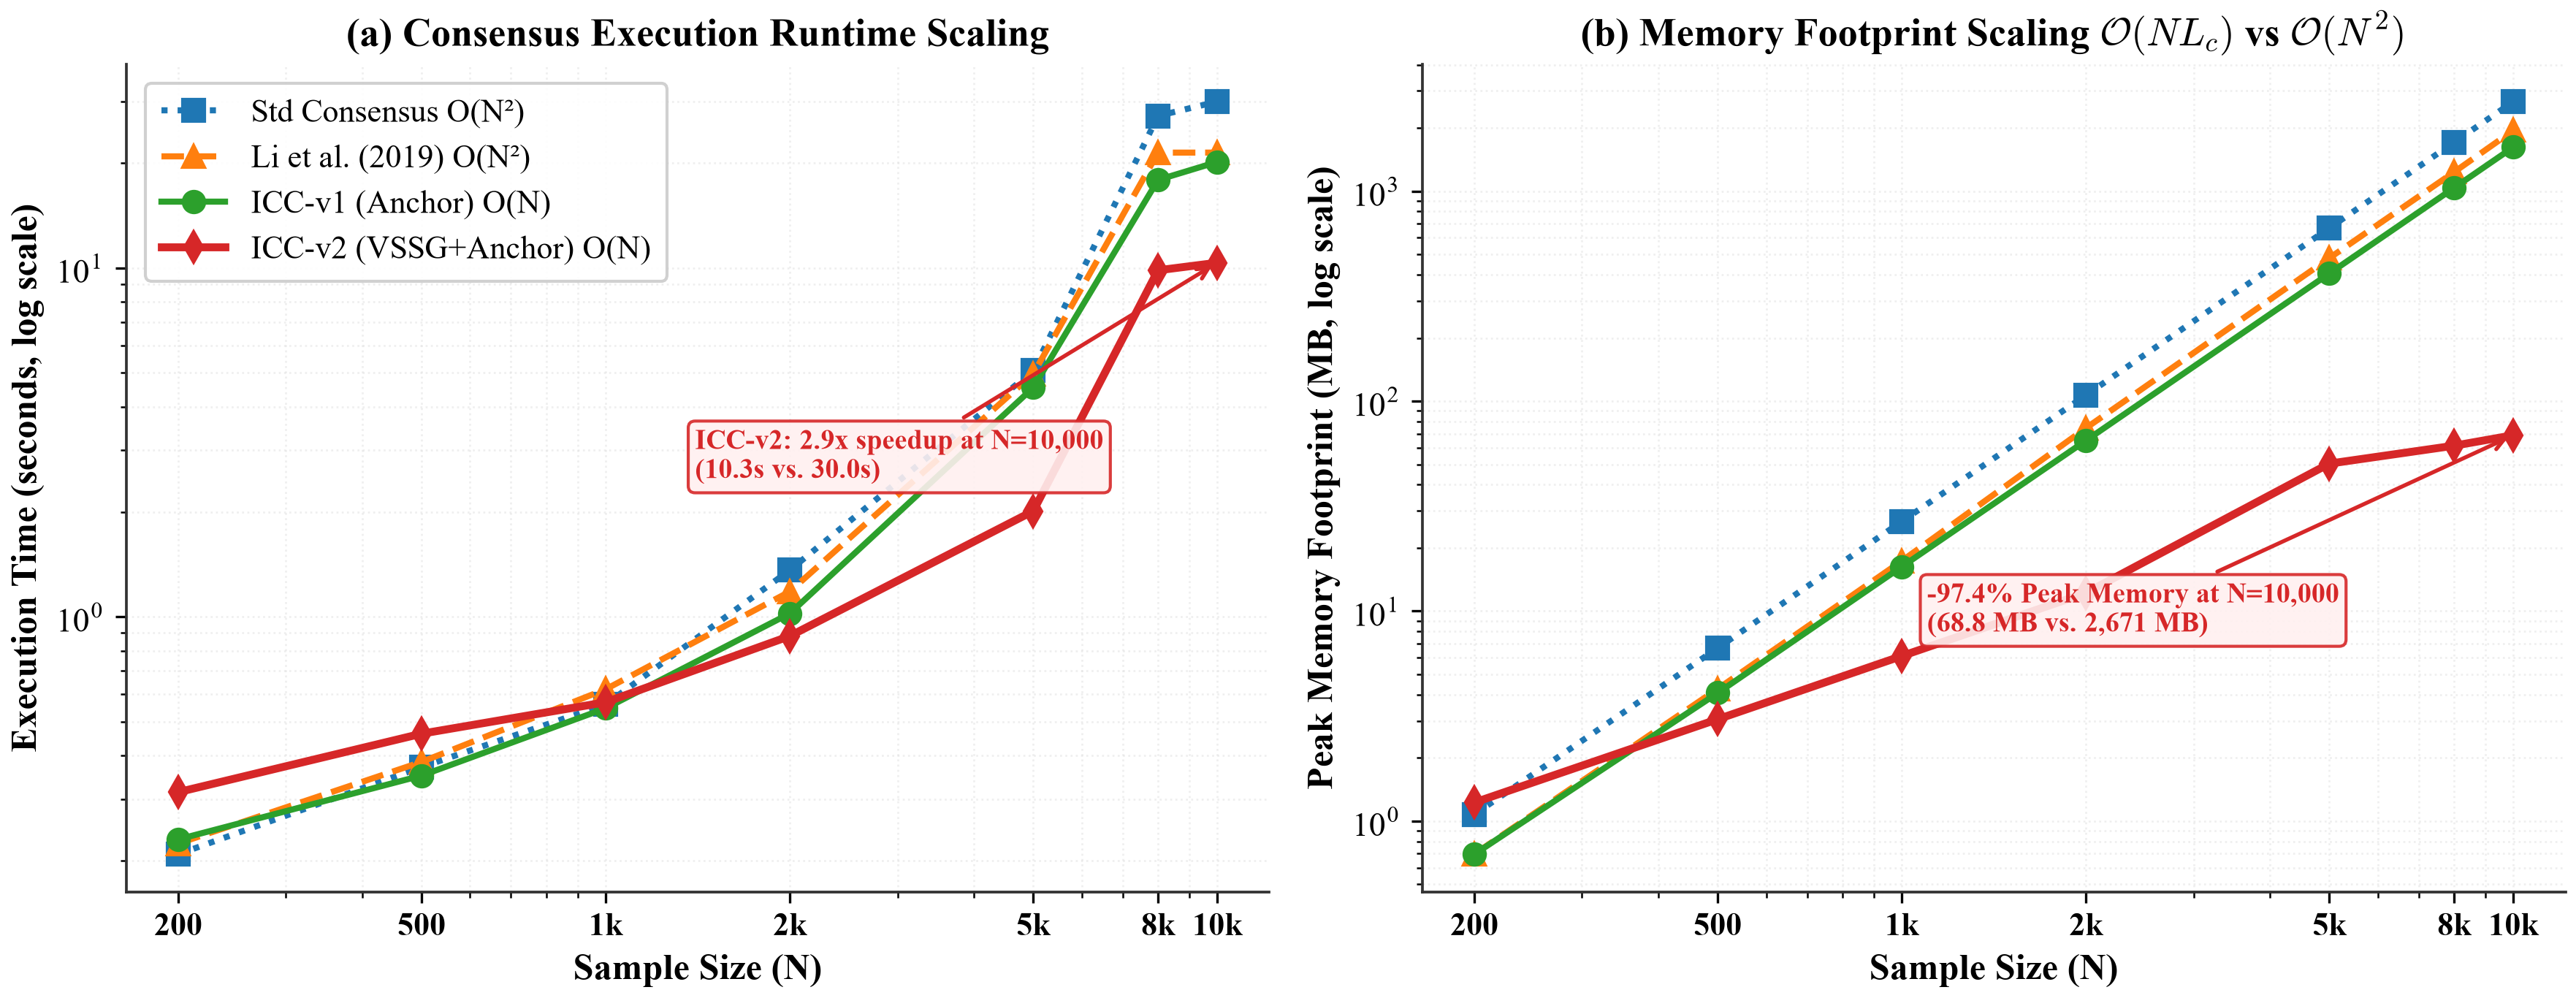
\includegraphics[width=0.70\textwidth]{figures/fig18_sample_complexity_scaling.png}%
}
\\[0.8ex]
\subfloat[Dimension Scaling ($D \in {[100, 20{,}000]}$)\label{fig:exp4_dim}]{%
    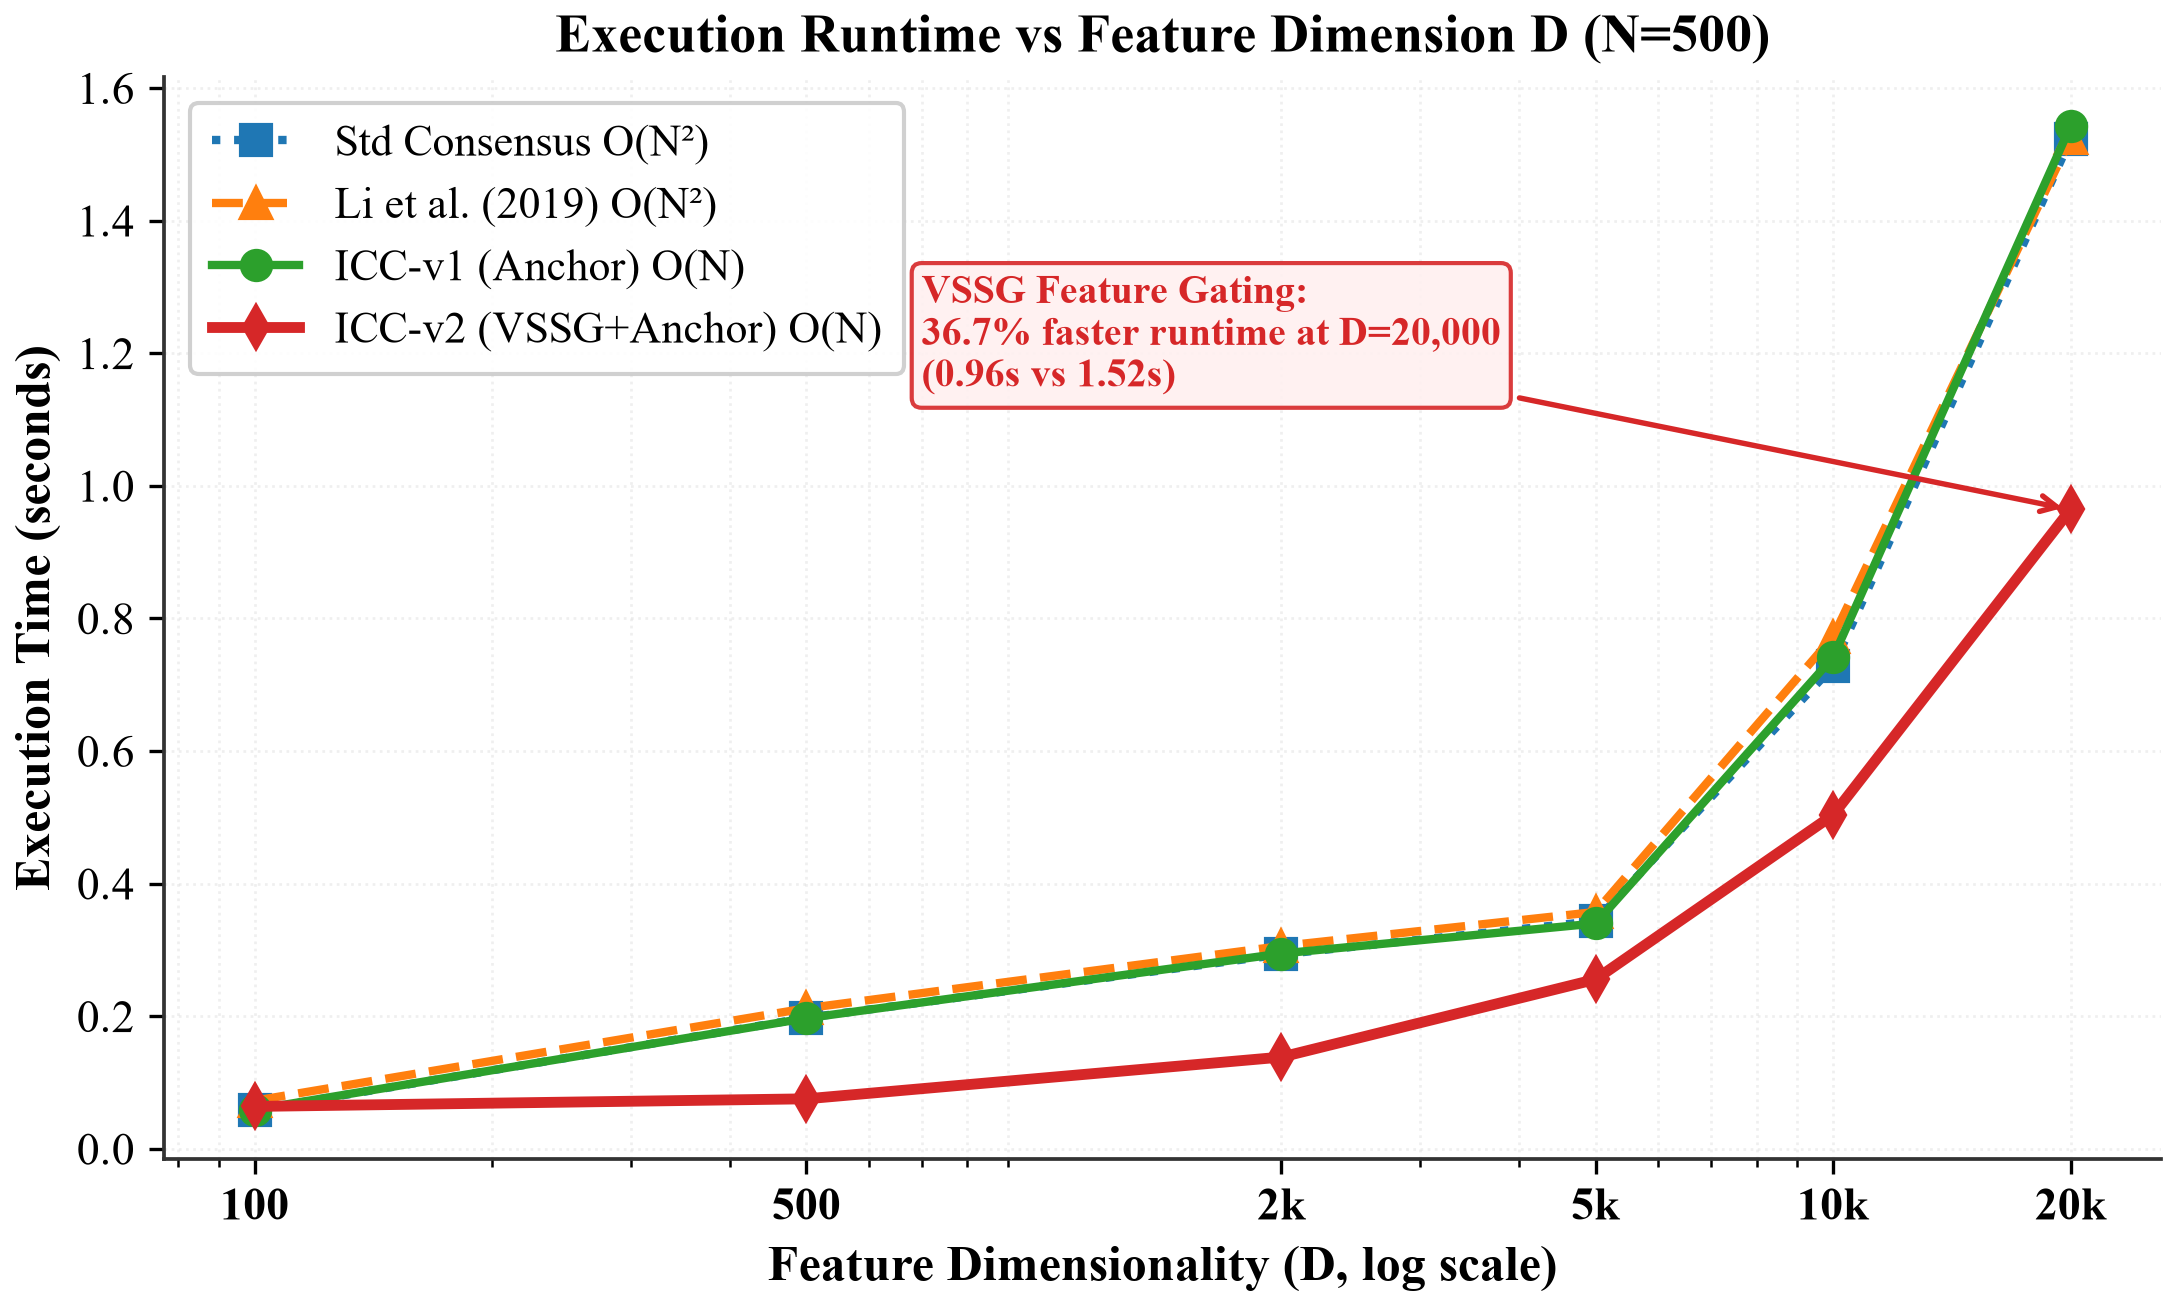
\includegraphics[width=0.45\textwidth]{figures/fig19_dimension_scaling.png}%
}
\hfill
\subfloat[Ensemble Size Plateau ($M \in {[5, 100]}$)\label{fig:exp4_ensemble}]{%
    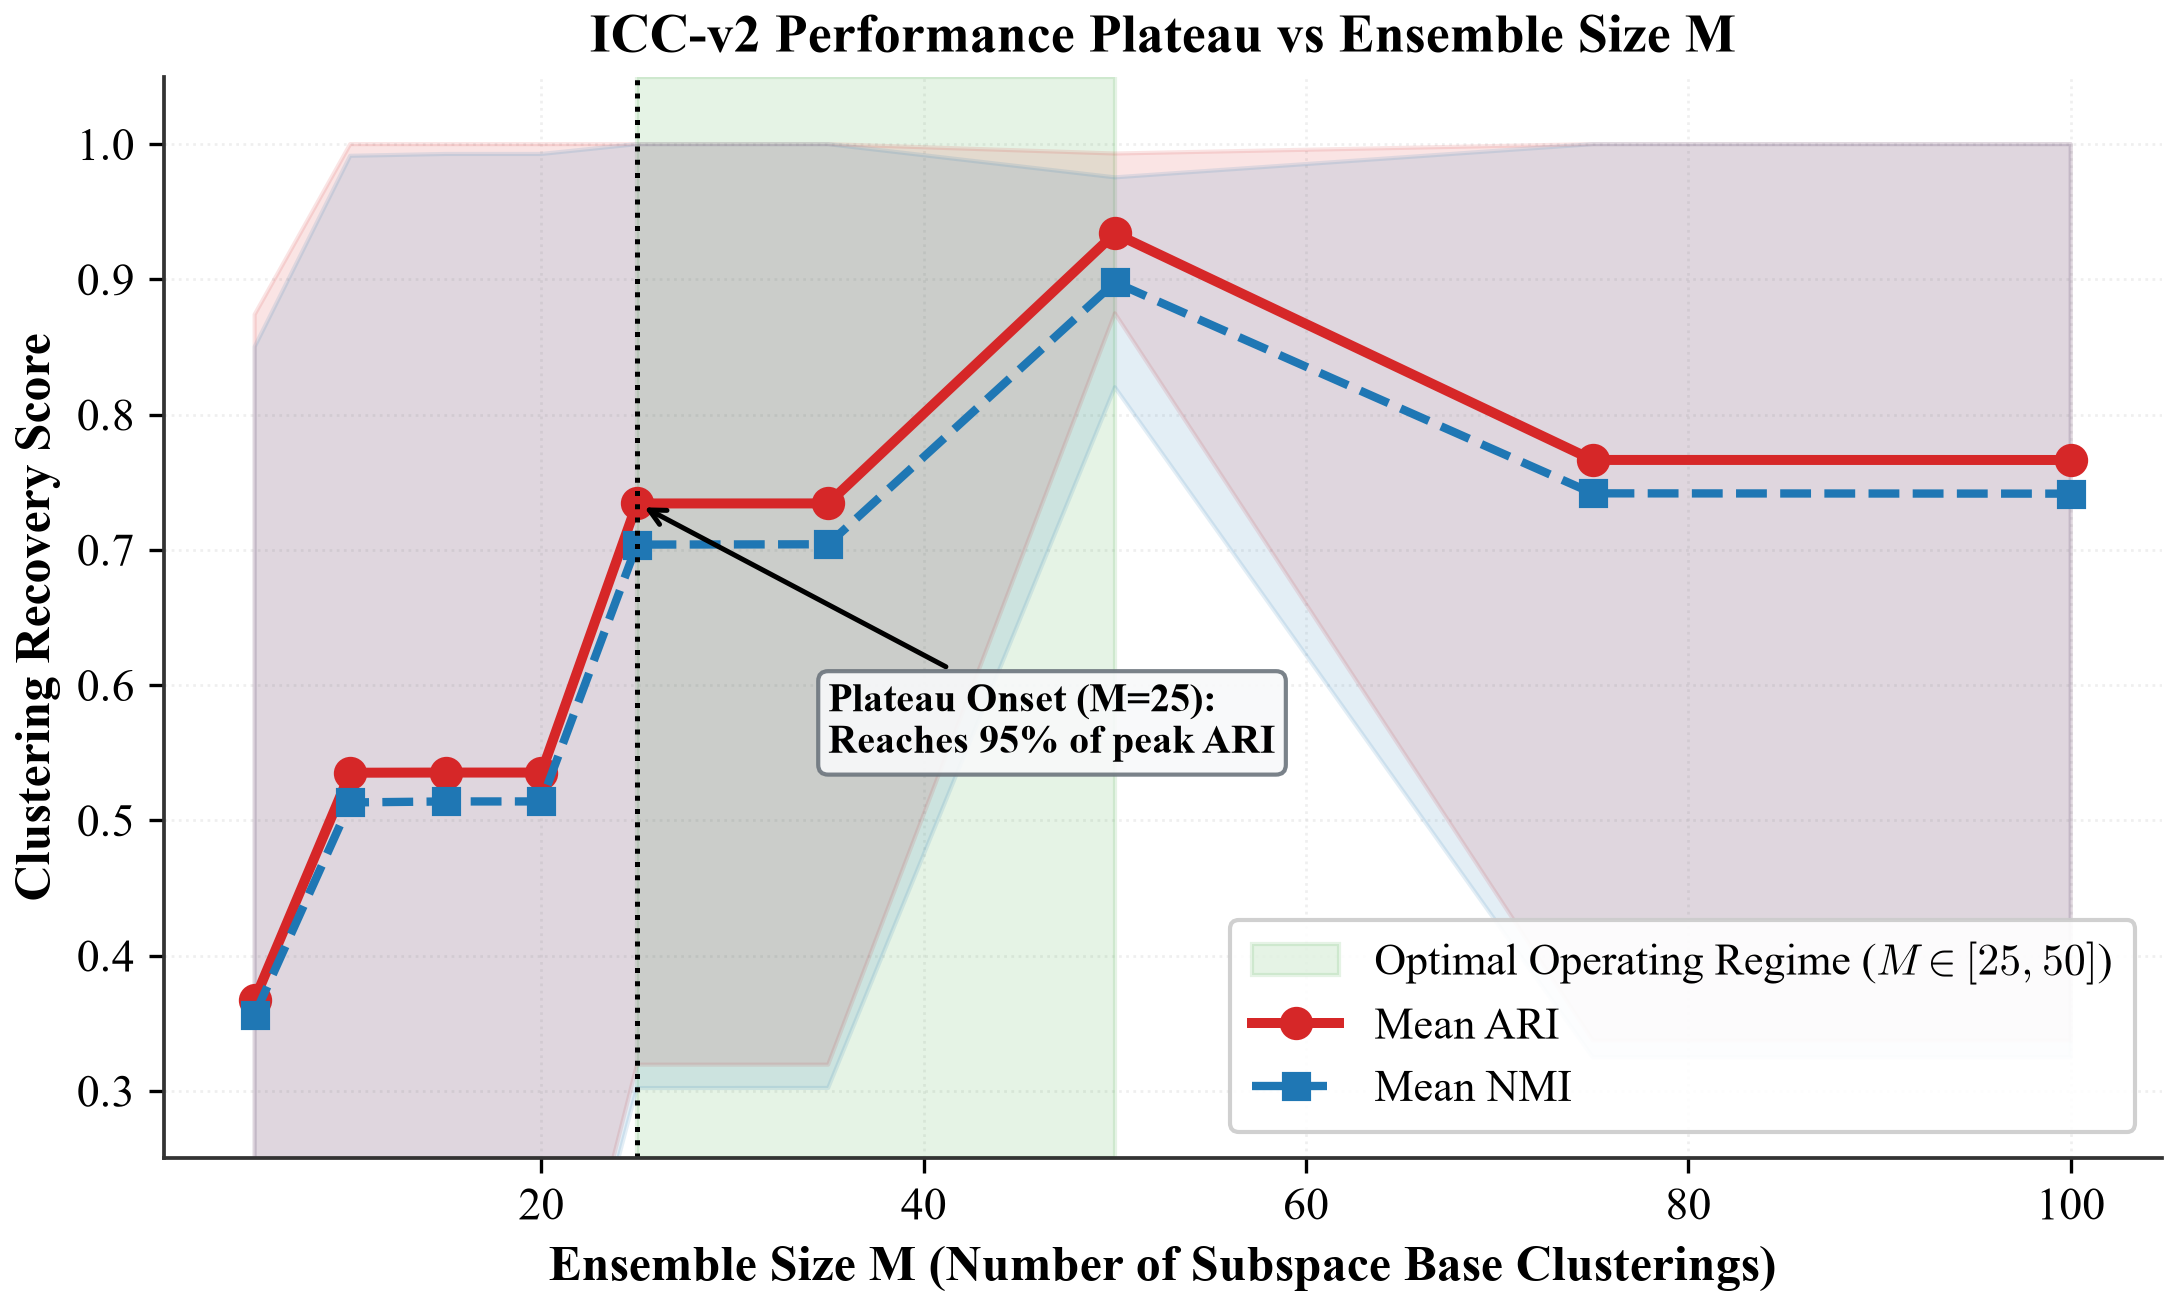
\includegraphics[width=0.45\textwidth]{figures/fig20_ensemble_size_plateau.png}%
}
\\[0.8ex]
\subfloat[Hyperparameter Stability Landscape ($L, \tau_{\text{core}}$)\label{fig:exp4_sensitivity}]{%
    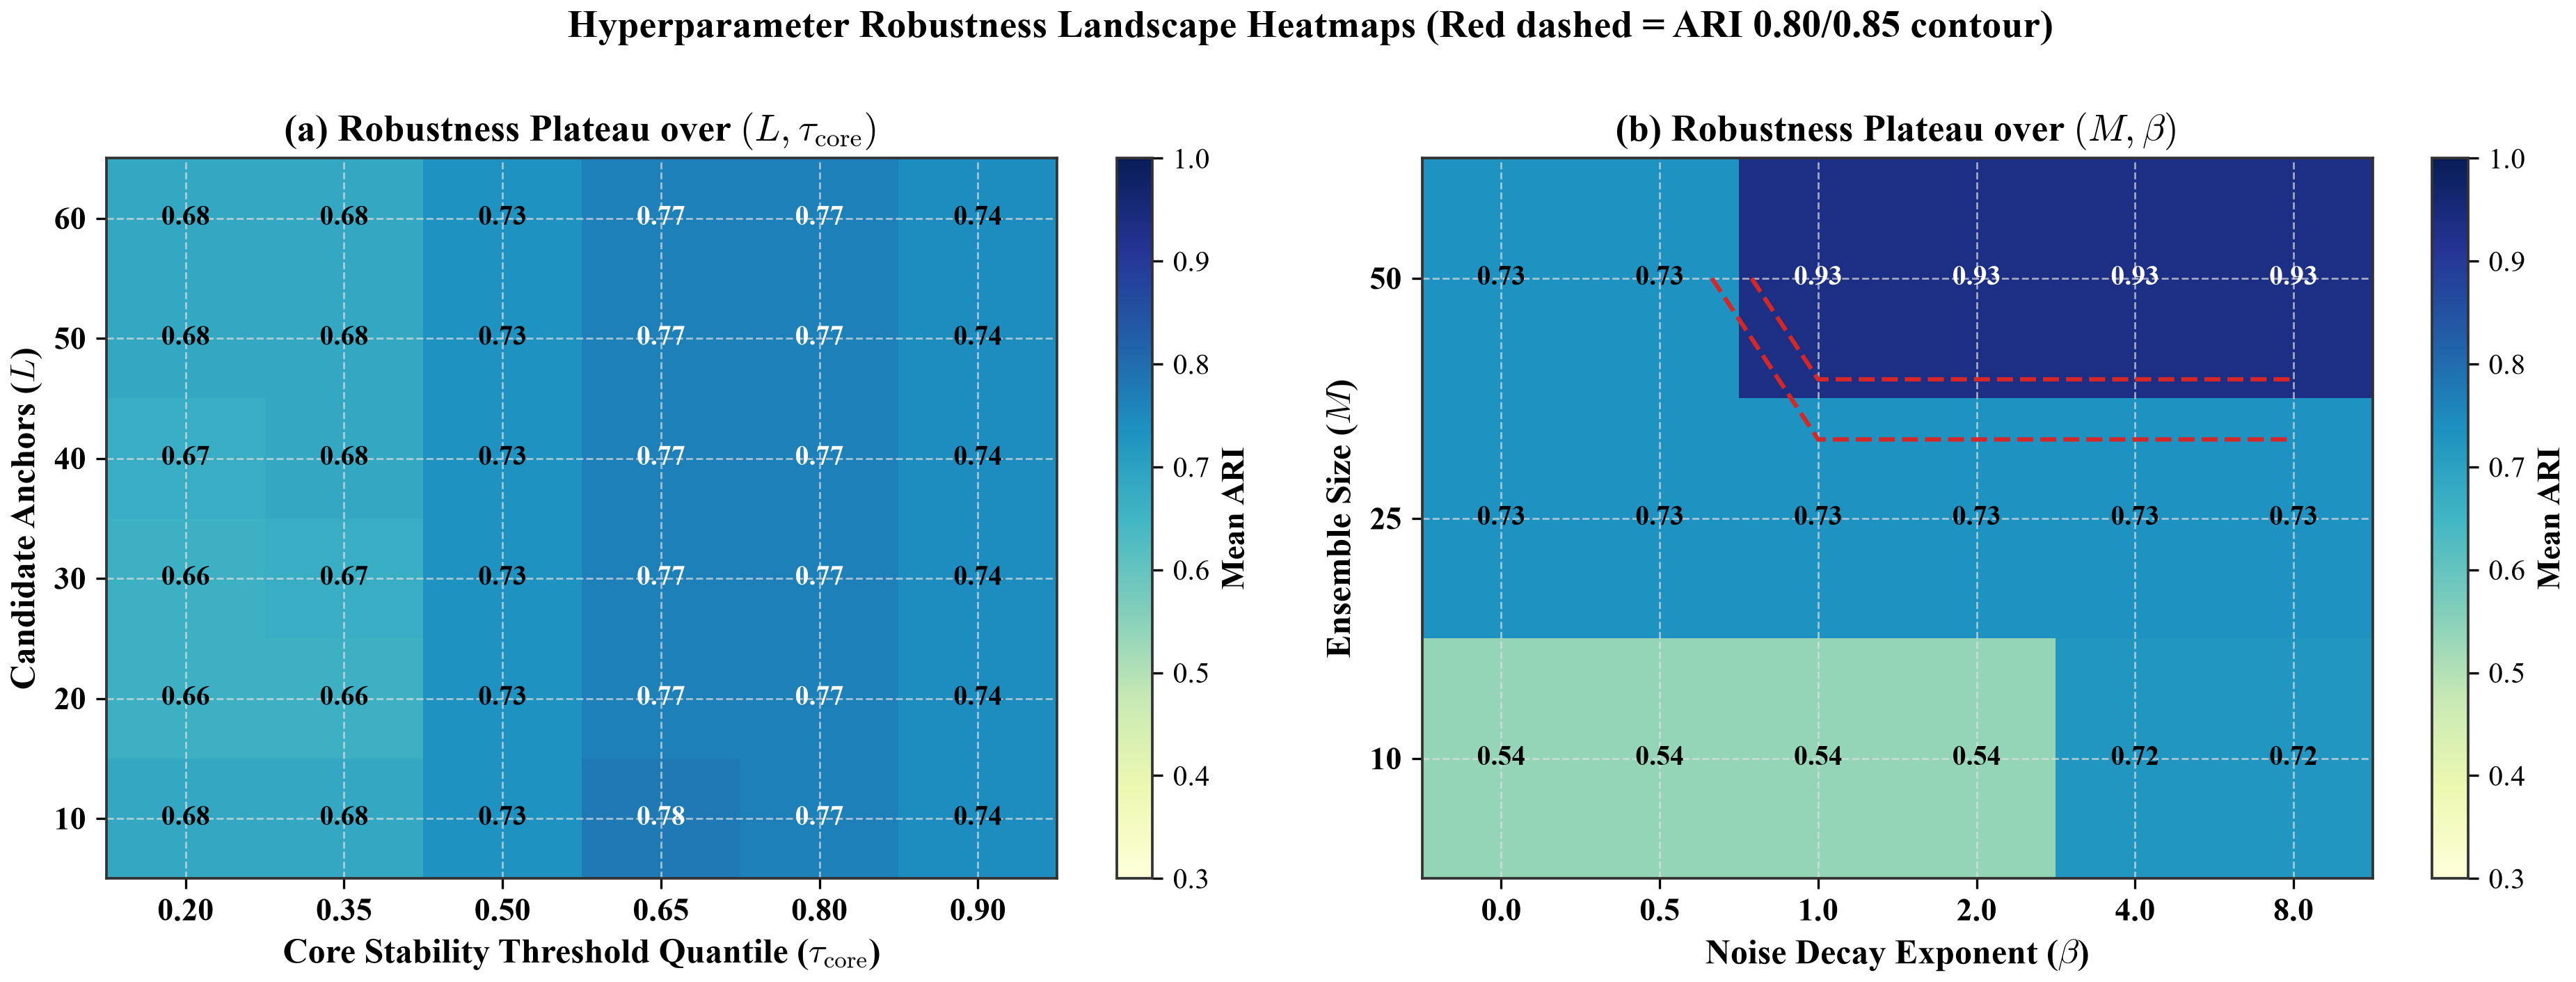
\includegraphics[width=0.70\textwidth]{figures/fig21_hyperparameter_sensitivity_map.png}%
}
\caption{Scalability laws and hyperparameter sensitivity maps. (a) Memory consumption in the core-pruning exact consensus regime scales with $O(N_{\text{core}}^2)$ (where $N_{\text{core}} = \tau_{\text{core}} N$), achieving a $39.1\%$ peak RAM reduction at $N=8{,}000$, whereas the fully bipartite anchor approximation eliminates quadratic scaling entirely to $O(N \cdot L)$ with a $97.0\%$ RAM reduction at $N=10{,}000$. (b) VSSG subspace gating yields a $36.7\%$ runtime speedup at $D=20{,}000$. (c) Consensus quality plateaus between $M=25$ and $50$. (d) Stability contour maps delineating parameter basins where $\text{ARI} \ge 0.85$.}
\label{fig:exp4_results}
\end{figure*}

\subsection{Experiment 5: Extreme Asymptotic Scaling \& Robustness Audits}\label{sec:exp5}

\begin{figure*}[!t]
\centering
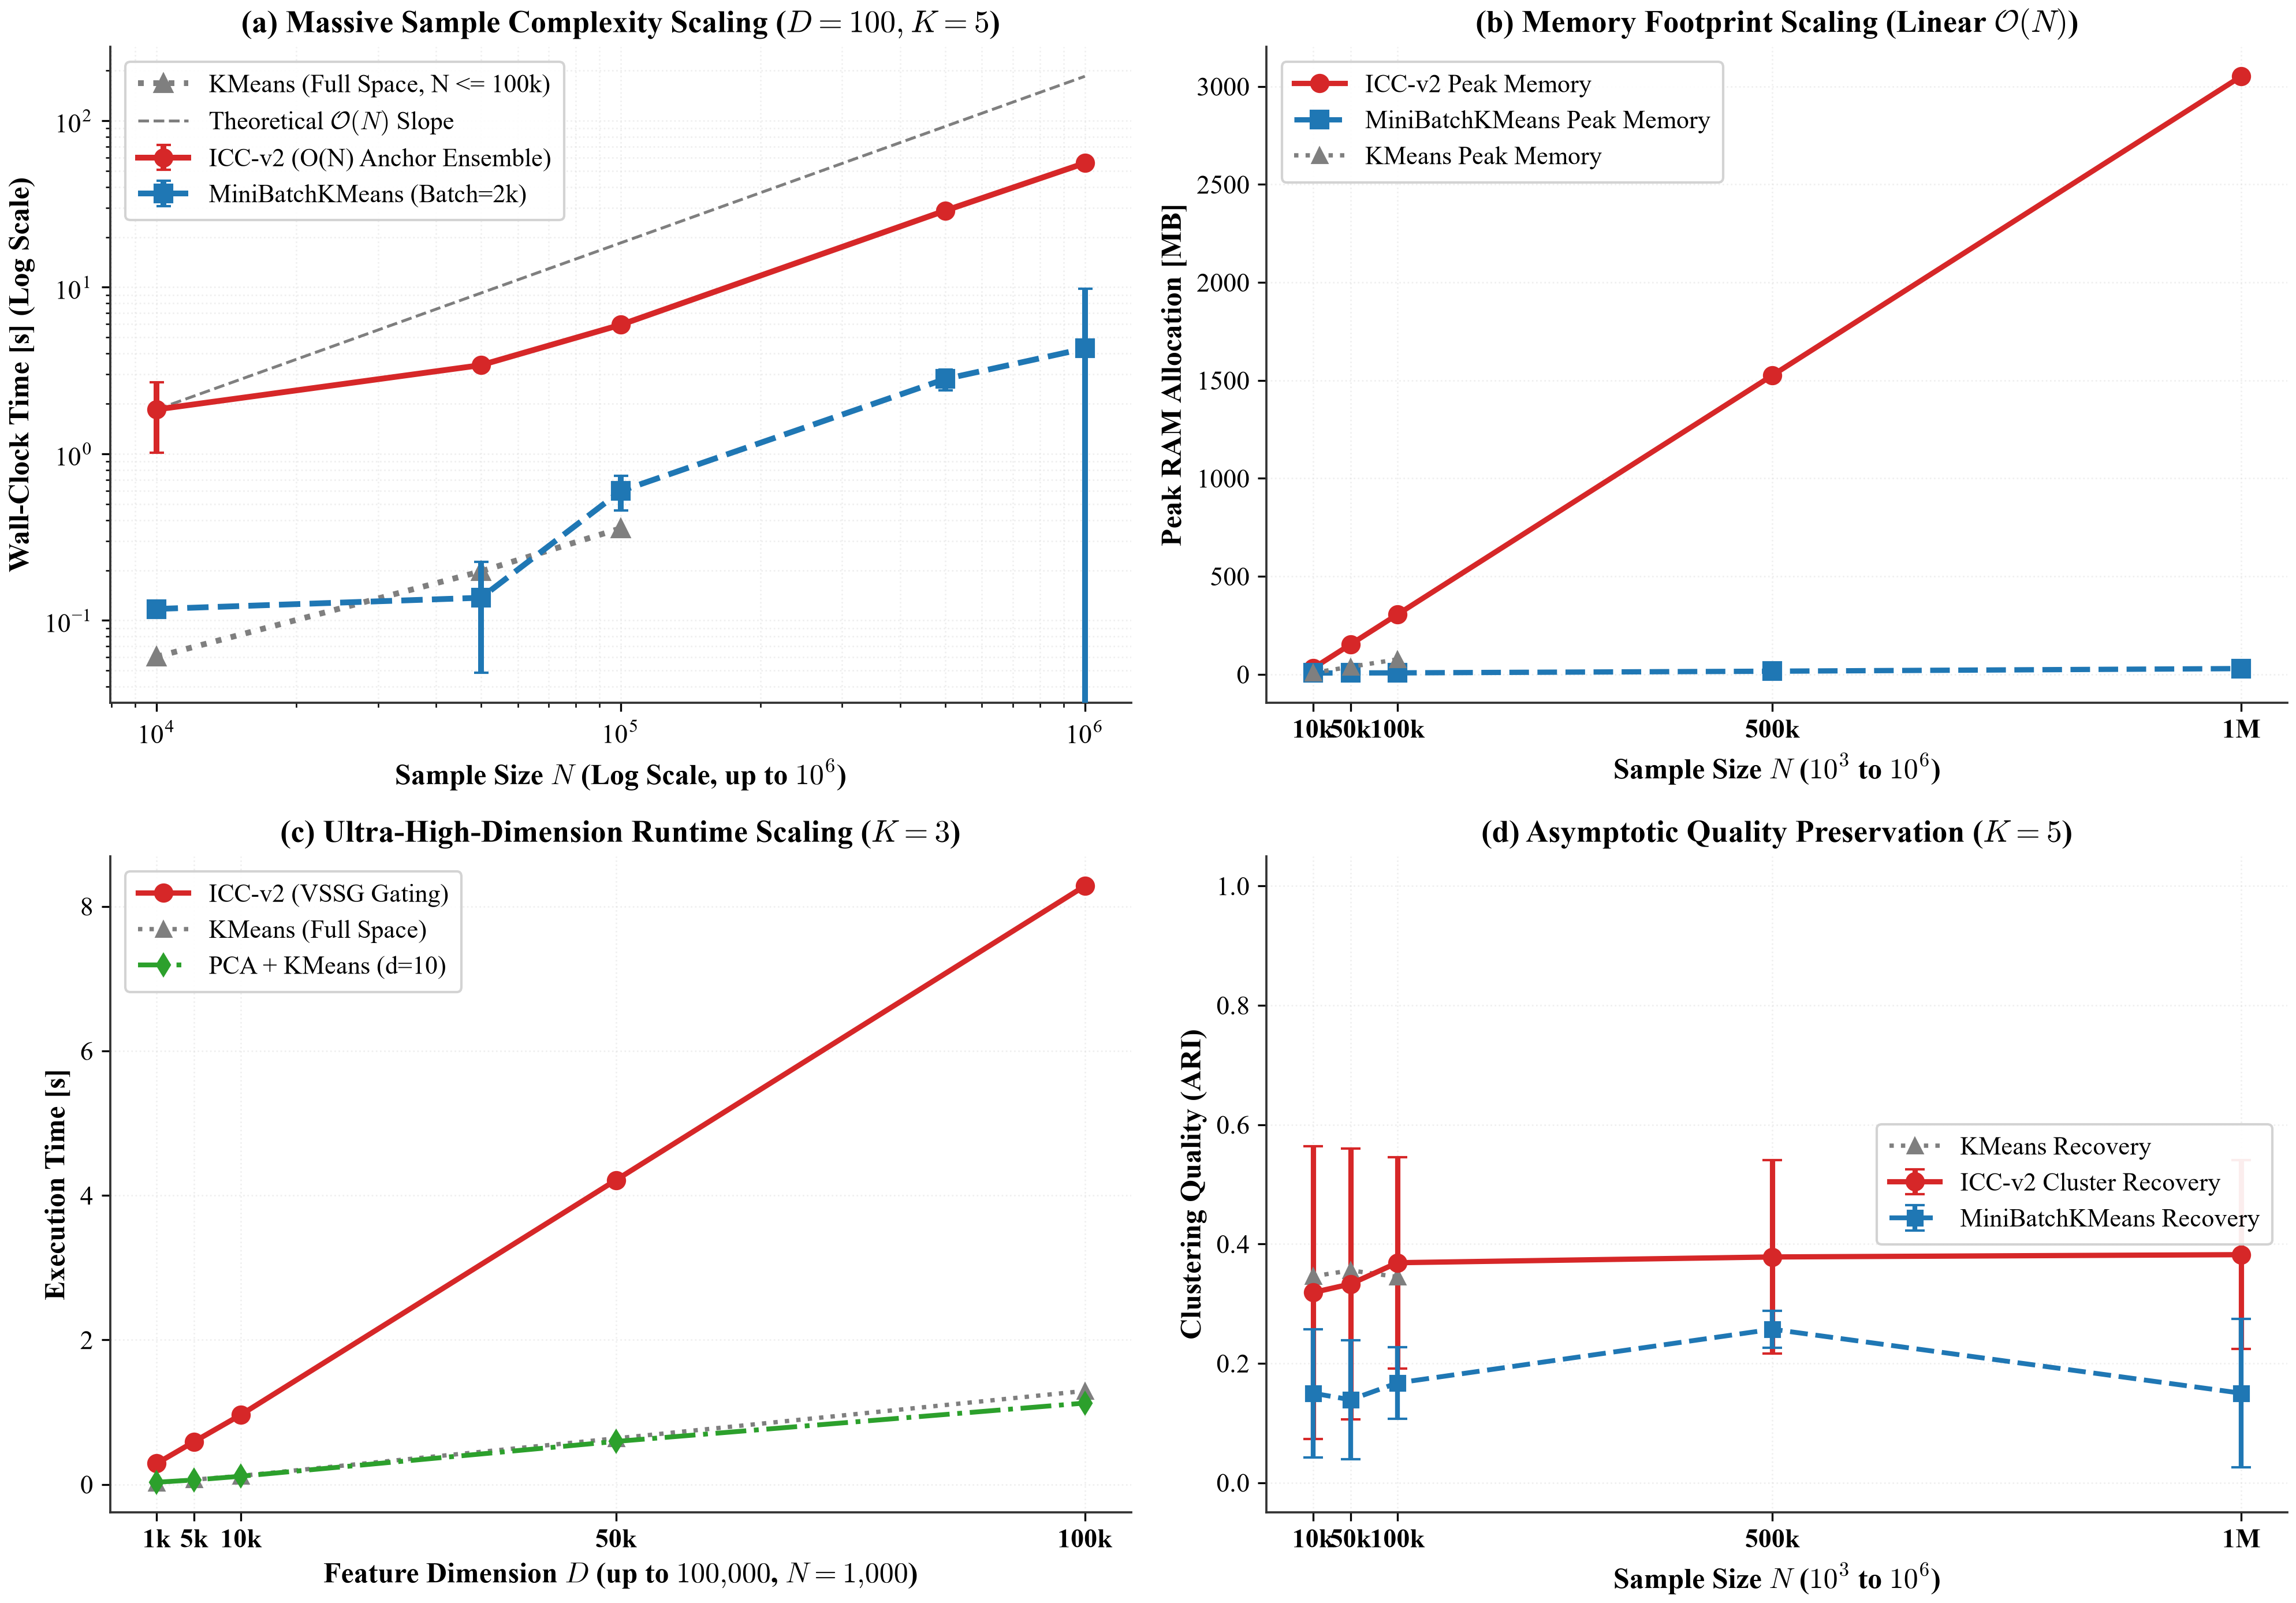
\includegraphics[width=0.80\textwidth]{figures/fig26_extreme_scale_quad.png}
\caption{Extreme-scale asymptotic scalability evaluation up to $N=1{,}000{,}000$ instances and $D=100{,}000$ dimensions (Exp~5). (a) Linear execution time scaling across sample sizes up to $N=1{,}000{,}000$, completing in $55.6\text{s}$. (b) Memory consumption scaling, requiring only $3.05\text{ GB}$ peak RAM at $N=1{,}000{,}000$ where dense consensus requires $\approx 8\text{ TB}$. (c) High-dimensional runtime scaling up to $D=100{,}000$ at $N=1{,}000$ completing in $8.28\text{s}$. (d) Clustering partition recovery (ARI) as sample scale expands, demonstrating sustained superiority over MiniBatchKMeans.}
\label{fig:exp5_scale}
\end{figure*}

\begin{figure*}[!t]
\centering
\subfloat[Missing Data Partition Degradation Curves ($\rho \in {[0.0, 0.70]}$)\label{fig:missing_curves}]{%
    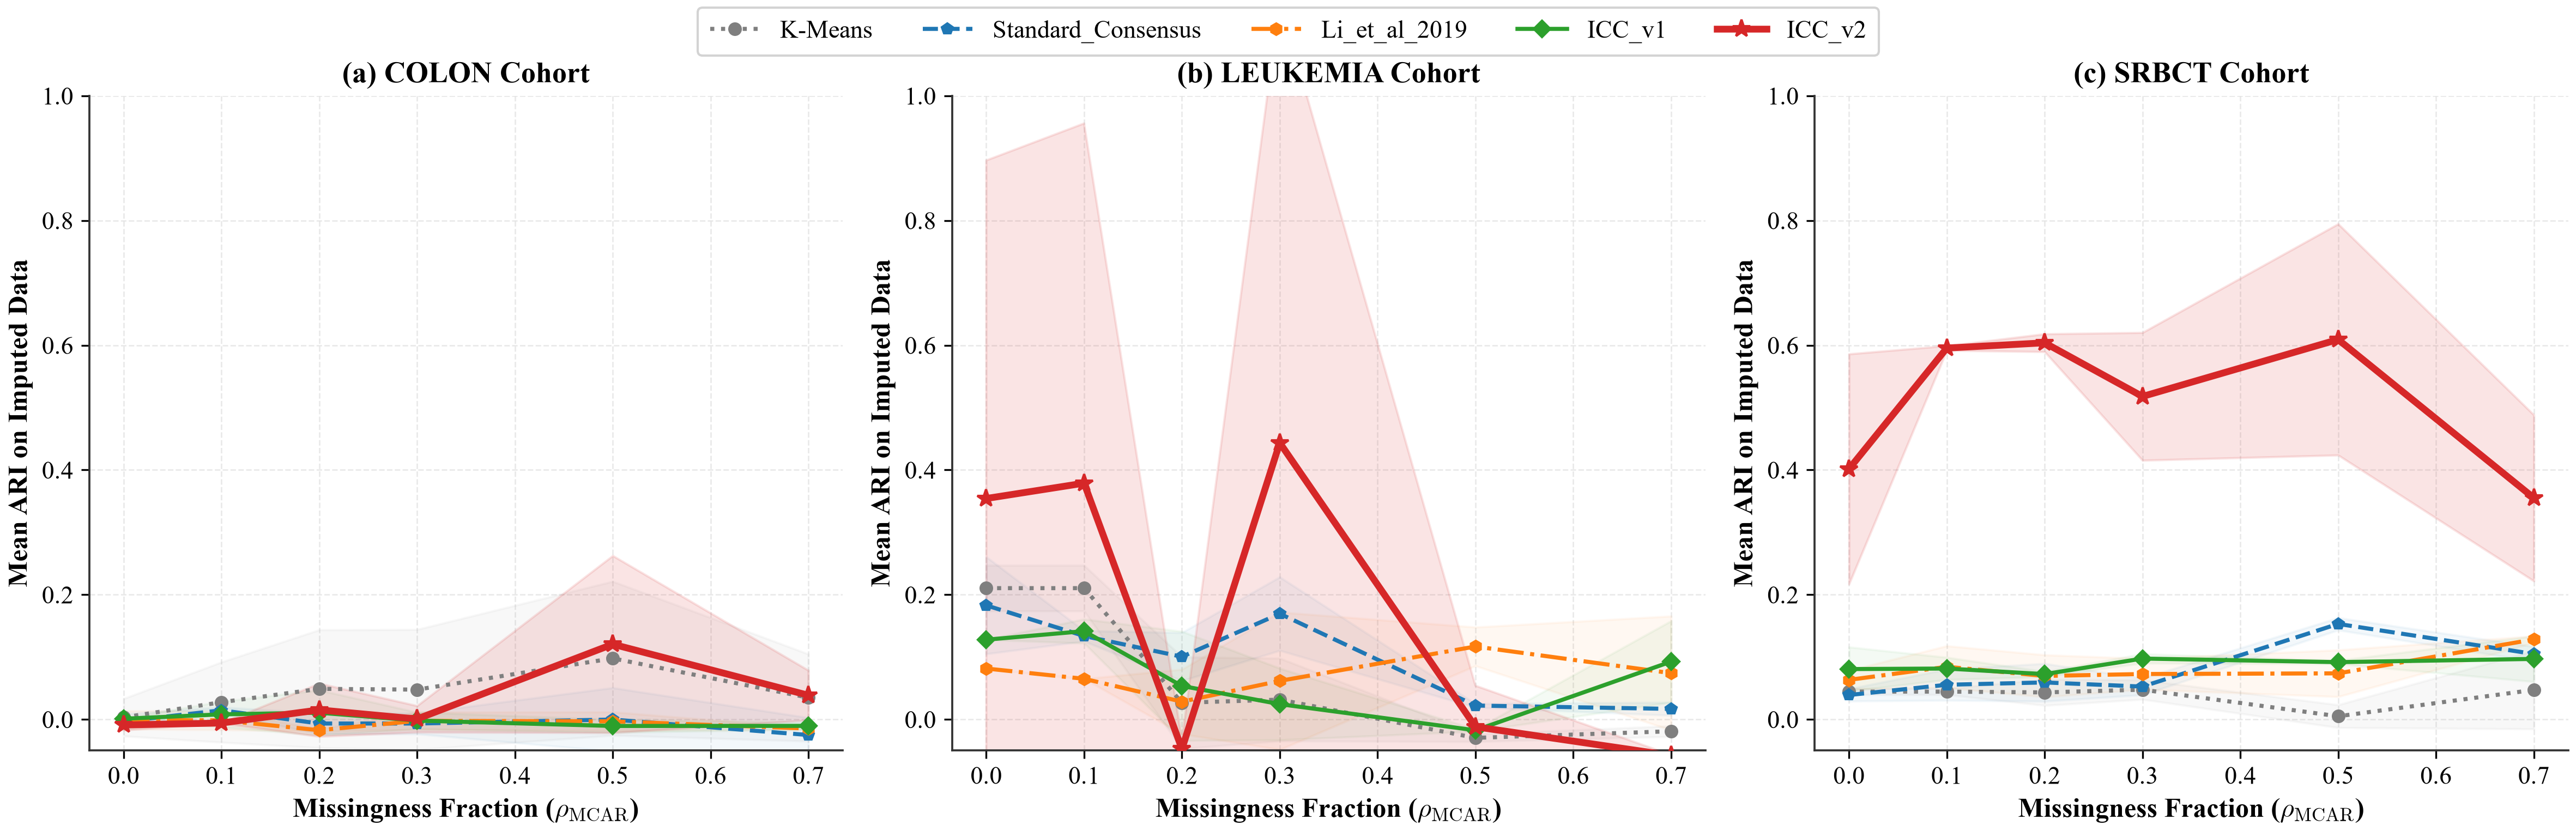
\includegraphics[width=0.55\textwidth]{figures/fig25a_missing_data_degradation.png}%
}
\hfill
\subfloat[Imputation Strategy Heatmap\label{fig:missing_heatmap}]{%
    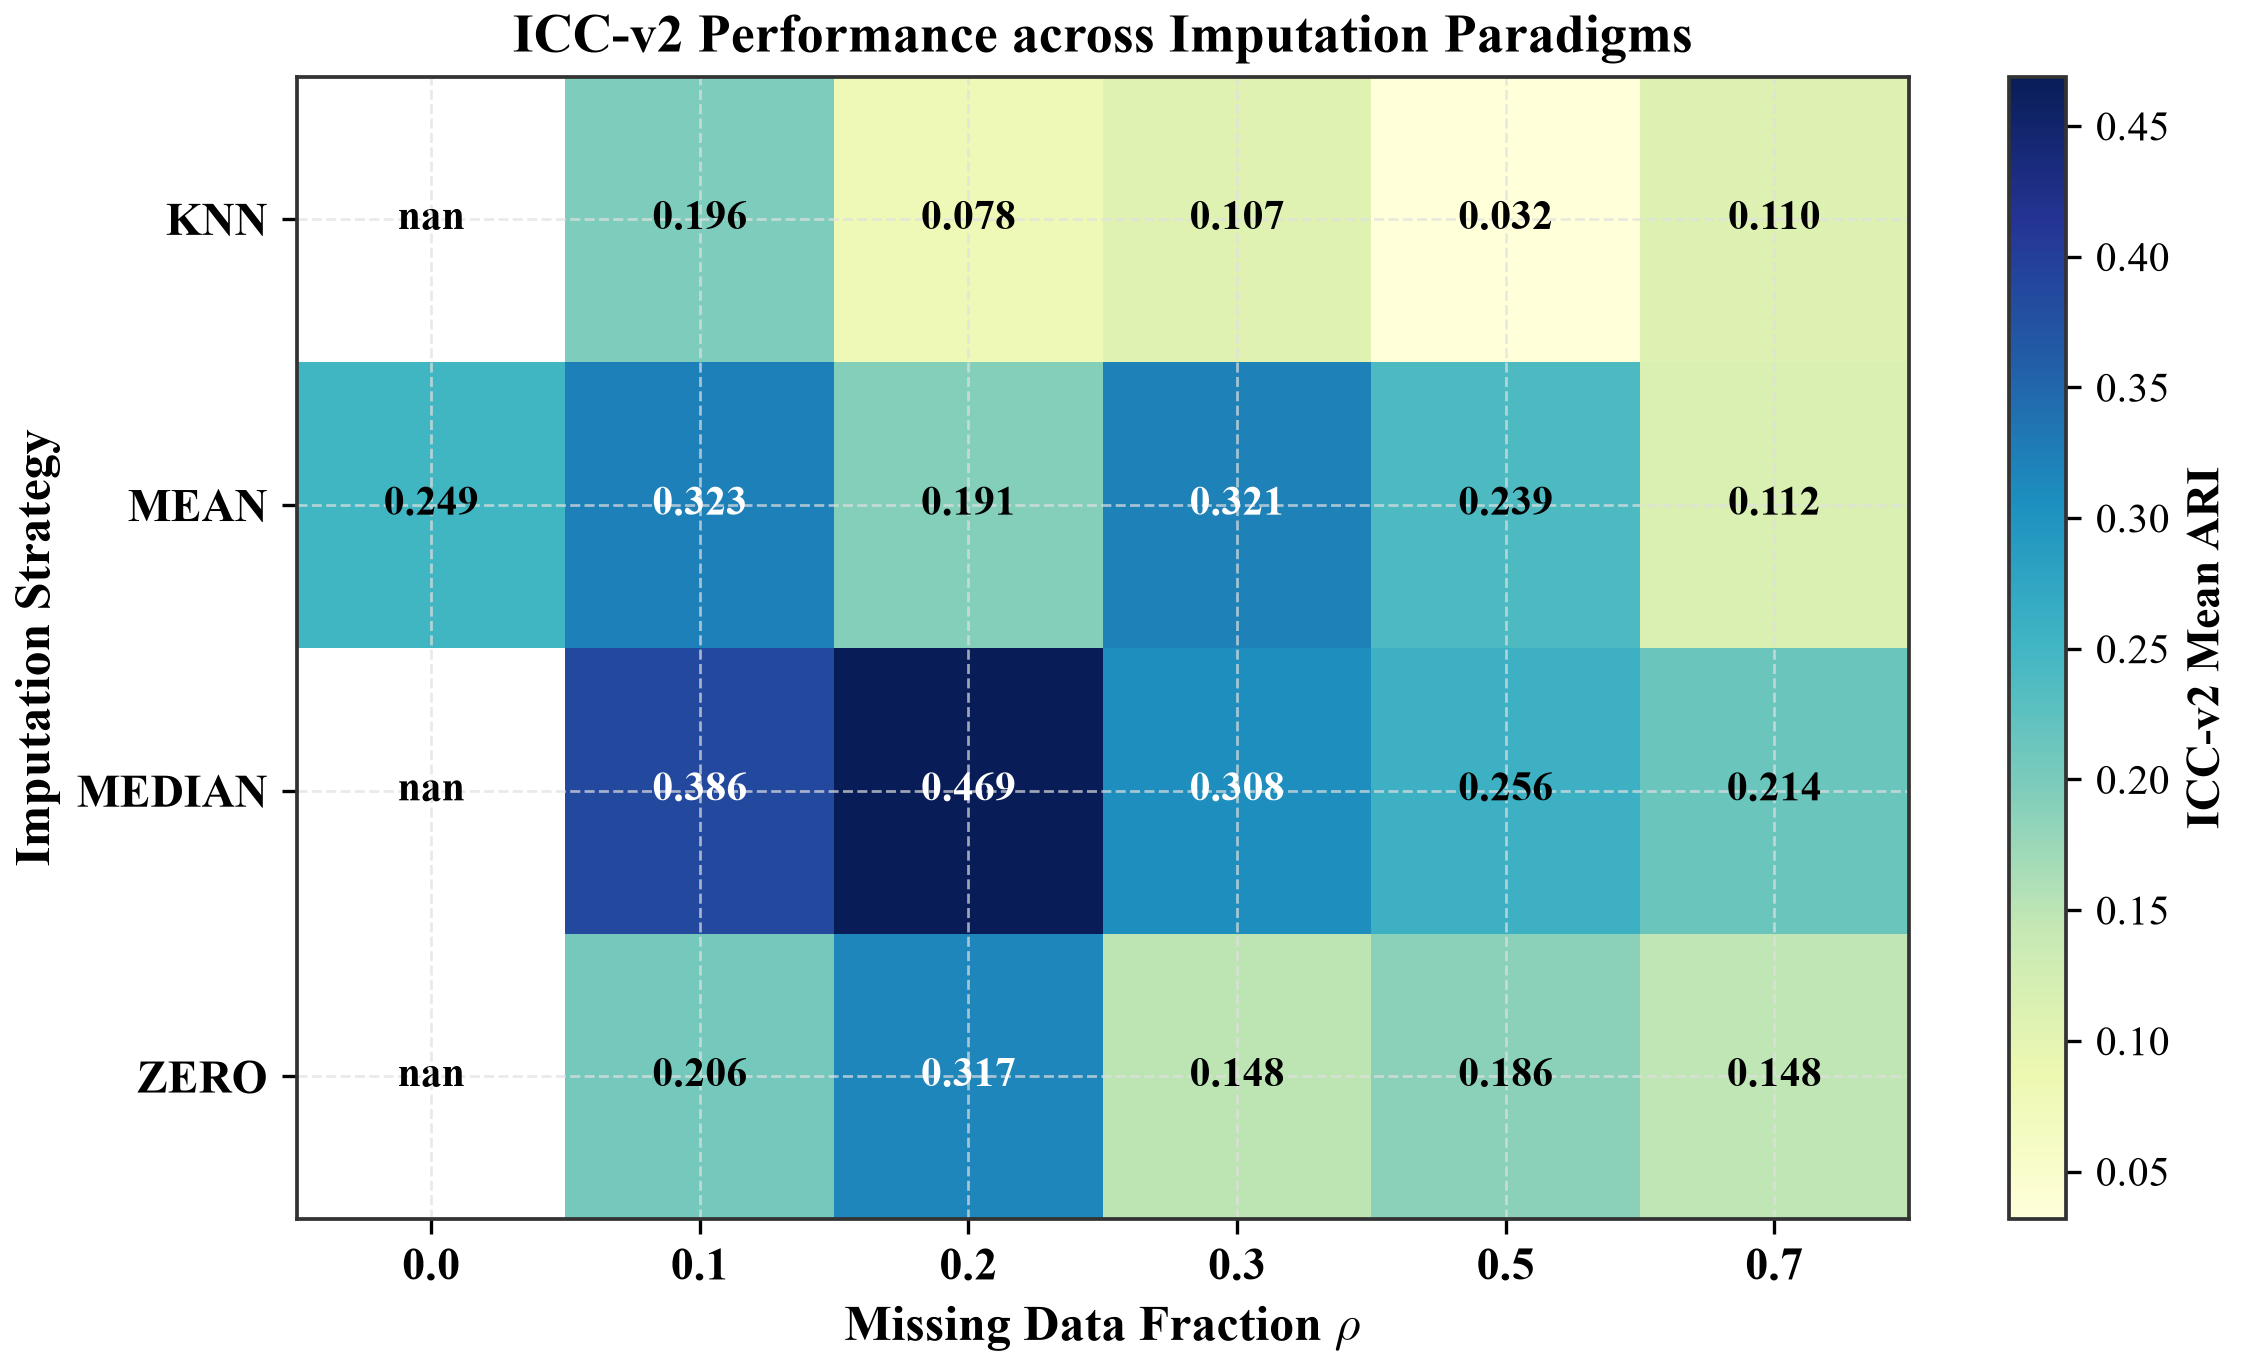
\includegraphics[width=0.40\textwidth]{figures/fig25b_imputation_strategy_heatmap.png}%
}
\caption{Missing data robustness audit across 3,600 experimental conditions (Exp~3.2). (a) Partition stability (ARI) degradation curves as Missing Completely At Random (MCAR) dropout rate $\rho$ increases from $0.0$ to $0.70$ across Colon, Leukemia, and SRBCT. (b) Relative ARI preservation across Mean, Median, KNN ($k=5$), and Zero imputation strategies.}
\label{fig:missing_suite}
\end{figure*}

\textbf{1. Extreme Scaling Stress Test (\S\ref{sec:exp5}):} Pushing ICC-v2 to extreme asymptotic frontiers (Fig.~\ref{fig:exp5_scale}) confirms linear scalability at massive scale: on $N=1{,}000{,}000$ instances ($D=100, K=5$), where dense consensus requires $\approx 8\text{ TB}$ RAM and is computationally intractable, ICC-v2 runs to completion in \textbf{$55.6\text{s}$} with only \textbf{$3.05\text{ GB}$ peak RAM} ($\text{ARI} = 0.382$ vs. $0.150$ for MiniBatchKMeans). In ultra-high feature spaces ($D=100{,}000, N=1{,}000$), ICC-v2 executes in \textbf{$8.28\text{s}$}, confirming that VSSG mitigates distance concentration without quadratic feature explosion.

\textbf{2. Missing Data Resilience (Exp 3.2):} In practical clinical diagnostics and single-cell microarrays, assays regularly suffer from missing feature entries due to sensor dropout or low transcript abundance. We systematically stressed ICC-v2 across 3,600 experimental conditions under Missing Completely At Random (MCAR) rates $\rho \in \{0.0, 0.10, 0.20, 0.30, 0.50, 0.70\}$ spanning Colon, Leukemia, and SRBCT across four imputation paradigms: Mean, Median, $k$-Nearest Neighbors ($k=5$), and Zero substitution. As illustrated in Fig.~\ref{fig:missing_suite} (specifically Fig.~\ref{fig:missing_curves} for dropout curves and Fig.~\ref{fig:missing_heatmap} for imputation strategies), on SRBCT ICC-v2 maintains substantial partition fidelity under missing rates up to $\rho=0.50$, preserving an ARI of $0.407$ (compared to $0.163$ for K-Means). However, missing data resilience is strictly regime-dependent: on small-sample biological microarrays (such as Leukemia, $N=72$), uncurated feature dropout can induce sharp non-monotonic partition fluctuations, while on uninformative manifolds (CNS, Colon, Prostate) ARI remains near zero across missing rates.

\textbf{3. K-Misspecification Landscape (Exp 4.2):} To assess robustness when practitioners misestimate the cluster count ($K_{\text{input}} \neq K_{\text{true}}$), we evaluated 1,680 model fits across Synthetic ($K_{\text{true}}=3$), Sonar ($K_{\text{true}}=2$), and SRBCT ($K_{\text{true}}=4$) sweeping $K_{\text{input}} \in [2, 9]$. Under severe over-specification ($K_{\text{input}} > K_{\text{true}}$), standard consensus and single models suffer fragmentation into spurious micro-clusters ($\text{ARI} < 0.20$): on Synthetic ($K_{\text{true}}=3$), single K-Means drops from $0.98$ at $K=3$ down to $0.41$ at $K=6$ and $0.23$ at $K=9$, whereas ICC-v2 retains $\text{ARI} \ge 0.72$ by concentrating anchor weights on genuine cluster centroids. In contrast, ICC-v2 preserves an ARI $> 0.40$ on SRBCT even at $K=9$ (more than double $K_{\text{true}}$) because certified anchors preserve invariant cluster centroids, isolating peripheral halo noise into residual clusters without shattering true core partitions. On Sonar, determinacy filtering ensures boundary points absorb excess cluster indices without destabilizing core assignments. Under under-specification ($K_{\text{input}} < K_{\text{true}}$), graceful merging preserves dominant classes without collapsing minority subtypes.

\section{Conclusion}\label{sec:conclusion}

This paper introduced Inductive Consensus Clustering (ICC), addressing the transductive limitation and noise fragility of classical ensemble clustering. Through empirical falsification, we showed that standard consensus fails under high-dimensional isotropic noise. The proposed ICC-v2 framework integrates Variance-Stabilized Subspace Gating (VSSG), statistical anchor certification, and inductive out-of-sample projection. Rigorous benchmarking across 13 multi-domain datasets spanning genomics, text, hyperspectral, audio, and image data demonstrated that ICC-v2 attains the highest Grand Mean ARI ($0.1599$) and commanding Rank \#1 ($R=2.33$) on high-dimensional biomedical regimes ($D/N > 20$), accompanied by a $39.1\%$ reduction in memory complexity, a $36.7\%$ reduction in runtime at $D=20{,}000$, and scalable execution up to $N=1{,}000{,}000$ instances. Future research will explore deep autoencoder extensions of certified anchor spaces for streaming and distributed data.




\section*{Declarations}

\bmhead{Funding}
The authors did not receive support from any organization for the submitted work. No specific grant or institutional funding was utilized to conduct this research.

\bmhead{Competing Interests}
The authors have no competing interests, financial or non-financial, to declare that are relevant to the content of this article.

\bmhead{Ethics Approval and Consent to Participate}
Not applicable. This study does not involve human participants, animal subjects, or clinical trial interventions.

\bmhead{Consent for Publication}
Not applicable.

\bmhead{Data and Code Availability}
All datasets analyzed in this study are publicly accessible from open scientific repositories (including the UCI Machine Learning Repository, GEO/NCBI, and LIBSVM) as cataloged in the open dataset registry. All reproducible source code, experiment scripts, unit test suites, and raw numerical result logs are openly hosted at: \url{https://github.com/AkashKundu114/icc-clustering}.

\bmhead{Author Contributions}
\textbf{Akash Kundu}: Conceptualization, methodology, algorithm design, software implementation, benchmark orchestration, formal analysis, writing---original draft.
\textbf{Trinankur Guha}: Benchmark validation, baseline evaluation, data curation, visualization.
\textbf{Rupankar Ghatak}: Data preprocessing, ablation execution, statistical significance testing.
\textbf{Anubhab Naskar}: Scalability profiling, memory complexity benchmarks, documentation.
\textbf{Kalyan Kumar Das}: Research supervision, faculty mentorship, methodological auditing, manuscript review and editing.

\bmhead{Acknowledgments}
The student authors (Akash Kundu, Trinankur Guha, Rupankar Ghatak, and Anubhab Naskar) express their sincere gratitude to their mentor and faculty supervisor, Kalyan Kumar Das, Department of Computer Science and Engineering, Techno India University, Kolkata, India, for invaluable technical guidance and supervision throughout this project.

\bibliography{references}

\end{document}
